\section*{Learning Objectives}

\begin{itemize}
    \item To introduce the concept and mathematical theory of Laplace Transforms.
    \item To become familiar with common Laplace transforms and their properties.
    \item To understand the process and methods of finding inverse Laplace transforms.
    \item To apply Laplace transforms for solving linear ordinary differential equations (ODEs).
    \item To define and derive transfer functions for linear time-invariant systems.
    \item To understand the importance and application of transfer functions in the design of Singe-Input Single-Output (SISO) feedback loops.
    \item To use appropriate software tools for each of the above topics.
\end{itemize}

\section*{Outcomes}

\begin{itemize}
    \item Gaining a foundational understanding of Laplace transforms and their application in engineering problems.
    \item Mastery of standard Laplace transforms of common functions and their key properties.
    \item Ability to understand inverse Laplace transforms using techniques such as partial fraction decomposition and tools in Julia.
    \item Proficiency in applying Laplace transforms to simplify and solve linear ODEs with initial conditions.
    \item Comprehensive understanding of transfer functions, their derivation, and significance in system analysis.
    \item Applying knowledge of transfer functions to design and analyze SISO feedback loops in engineering systems, particularly in robotics.
\end{itemize}



% \section*{Remarks for Jessy}

%  \begin{enumerate}
% \renewcommand{\labelenumi}{(\alph{enumi})}
% \setlength{\itemsep}{.2cm}
%     \item  I need an exploded view of the Segway to motivate moment of inertia computations for rotating wheels, motor rotors, platform, human body, etc. 
%     \item This will add realism to the integration Chapter, and tie it together with Lagrange, etc. 
% \end{enumerate}
\newpage

\begin{center}
\setlength{\fboxrule}{2pt}  % Setting the thickness of the border line
   \fbox{ \parbox{0.9\linewidth}{
   \vspace{.15cm}    
   \textcolor{blue}{\bf The Laplace Transform Magically Turns Linear Differential Equations into Algebraic Equations.} \textbf{
One of the most remarkable aspects of Laplace Transforms lies in their ability to transmute the complexities of linear ODEs into the more tractable realm of algebra.} This metamorphosis is not merely a theoretical curiosity but an immensely practical tool that unlocks a new perspective on ODEs. \textcolor{blue}{\bf By translating the differential equations into algebraic ones, Laplace Transforms simplify the process of understanding solutions of ODEs, showing how to modify the equations to achieve asymptotic stability.} \textbf{This technique allows for a more straightforward analysis and design of systems governed by ODEs, thereby bridging the gap between complex mathematical theory and real-world application.
} 
}
} 
\end{center}
\vspace*{.2cm}

\section{Introduction}


Thanks to Chapter~\ref{chap:ODEs}, we now understand what an ODE is, how to compute its solution for given initial conditions, and whether its solutions asymptotically converge to an equilibrium point or not. That is already a big accomplishment. We now make a radical change in focus from analyzing solutions of ODEs to actively modifying their solutions so that they exhibit properties that we deem desirable. To achieve this, we introduce controlled inputs into our ODE models of physical systems. These inputs serve as a mechanism to influence and steer the evolution of the system's state. By strategically manipulating these inputs, we can guide the system's trajectory toward our objectives, such as achieving exponential stability, driving an important signal to a desired value (e.g., setting a robot's speed), or attenuating the effects of perturbations. This approach marks a significant shift from passive analysis to active control, opening the door to designing systems that respond effectively to commanded inputs and achieve specific, desired outcomes.

The fascinating possibilities of feedback control are introduced within the context of linear Single-Input Single-Output (SISO) systems, utilizing Laplace Transforms and transfer functions. We employ the Segway model as a practical example to demonstrate the foundational principles of feedback control, while also touching upon concepts like PD controllers and pre-compensators. Through our exploration of Laplace Transforms and transfer functions, we aim to provide an initial framework for understanding how these tools can be used to design basic yet effective feedback control strategies. The chapter builds upon the concepts of stability and feedback introduced in Chapter~\ref{chap:ODEs} and Example~\ref{ex:StabilizeNonlinear2LinkRobotArmUpwardEquilibrium}, illustrating the impact of these tools in engineering. Our principal goal is to provide the concepts and methods required for stabilizing the BallBot mobile robot used in ROB 311 Build Robots and Make Them Move. 

Appendix A offers further insights for readers seeking a deeper dive into the subject of Feedback Control. It's important to note, however, that even this additional material, while illustrative and intriguing, remains an introductory overview and is not a substitute for more advanced courses such as Michigan's EECS 460 Control Systems Analysis and Design, ME 461 Automatic Control, ROB 498.002 Robot Controls, or any of the other amazing Control Courses listed \href{https://controls.engin.umich.edu/control-courses/}{here}.  \\



\begin{figure}[hbt]
\centering
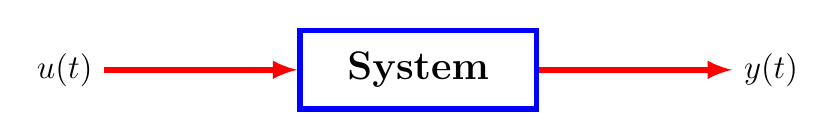
\begin{tikzpicture}[scale=3.5] % Adjust the scale factor as needed
    % Define arrow length
    \def\arrowLength{0.7}
    
    % Box for the system with thick blue border
    \node[draw, rectangle, minimum height=1cm, minimum width=3cm, thick, draw=blue, line width=2pt] (system) {\Large \bf System};
    
    % Arrow for input u(t) pointing towards the system with red line and black text
    \draw[->, >=latex, red, line width=2pt, text=black] ([xshift=-\arrowLength cm]system.west) node[left] {\large $\bm{u(t)}$} -- (system.west);
        
    % Arrow for output y(t) exiting from the system with red line and black text
    \draw[->, >=latex, red, line width=2pt, text=black] (system.east) -- ([xshift=\arrowLength cm]system.east) node[right] {\large $\bm{y(t)}$};
\end{tikzpicture}
    \caption[An Input-Output System]{An Input-Output System. The signal \(u(t)\) represents the action of an \href{https://en.wikipedia.org/wiki/Actuator}{actuator}, such as a DC motor, a rocket engine, or a voltage supply. The output is a signal that is important to the system designer, such as the speed of a robot or the angle of a joint. If $u(t)$ are $y(t)$ are scalar-valued, then one has a Single-Input, Single-Output (SISO) System. If $u(t)$ or $y(t)$ are vectors, then one has a Multi-Input Multi-Output (MIMO) System.}
    \label{fig:SISOsystemDiagram}
\end{figure}

% To adjust the boldness of the lines, you can modify the line width parameter in the \draw commands. For example, changing line width=1pt to line width=2pt will make the lines bolder.

% To adjust the font size of the labels, you can use standard LaTeX font size commands. For example, to make the font larger, you could change node[left] {$u(t)$} to node[left] {\Large $u(t)$}.

% You can also adjust the size of the system box by modifying the minimum height and minimum width parameters in the \node command.

\section{Single-Input Single-Output (SISO) Linear Systems}

A system is an ODE with both inputs and outputs. A drone (aka, quadrotor) is a system. A system's inputs are signals that cause changes in the motion of the entire system or parts of the system. A quadrotor-drone has four DC motors with propellers attached to them. These are the actuators. The output of the drone could be its 3D position and its 3D orientation in $\real^3$. A simpler output would be its speed in a single direction, say along the $x$-axis. It would be up to you (or your team, or your boss) to define the important quantities to be regulated in the system. Here, we define linear systems with a single input and output. It's THE PLACE to start. The planar Segway model that will guide our discussion has one input (a motor at the wheels) and two outputs (the angle of the Segway's body and its speed) that we will learn to treat successively. Controlling two outputs with one input is more challenging than controlling one output. C'\'est la vie, b\'eb\'e! That's Robotics in a nutshell. \\

\subsection{Input-Output and State-Variable Models}

Every domain has its ``secret codes and rituals''. In \textbf{Feedback Control}, the generic notation for an input is $\bm{u(t)}$, and for an output, $\bm{y(t)}$. We will use this notation so that you are not caught off guard in a follow-on course.


\vspace*{.2cm}

\begin{tcolorbox}[colback=mylightblue, title = {\bf SISO Linear Systems}, breakable]

\begin{definition}
\label{def:LinearIOsystem} 
\begin{equation}
\label{eq:LinearIOsystem}
y^{(n)} + a_{n-1} y^{(n-1)} + a_{n-2} y^{(n-2)} +  \cdots +  a_1 \dot{y} + a_0 y = b_0 u + b_1 \dot{u} + \cdots + b_m u^{(m)}
\end{equation}
is a \textbf{linear input-output system}. It is called an input-output system because the only variables present are the input, the output, and their derivatives. Because we will always assume that both $u(t)$ and $y(t)$ are scalars, it is a \textbf{SISO linear system}.  \\
\end{definition}

\vspace*{.2cm}
\textbf{Note:} We are taking the coefficients $a_k$ to be constants. In this case, the model is called a \textbf{Linear Time-Invariant (LTI)} input-output system. If the coefficients depend on time, then one has a \textbf{Linear Time-Varying (LTV)} input-output system. Even grad students struggle with LTV models, so don't worry, we're not going there. 
\vspace*{.2cm}

\begin{definition}
\label{def:LinearStateVariableModel} 
Consider a linear system of ODEs, $\dot{x} = Ax$, with $x \in \real^n$. It becomes a \textbf{control system} if we add an input and an output to the model. In particular, for $b$, an $n \times 1$ column vector and $c$, a $1 \times n$ row vector, 
\begin{equation}
\label{eq:LinearStateVariableModel}
\begin{aligned}
    \dot{x} &= Ax + b u \\
    y &= c x
\end{aligned}
\end{equation}
is a \textbf{SISO linear state variable model}. While studying MIMO linear state variable models is super interesting, we will not do that. \\
\end{definition}

%\vspace*{.2cm}
\textbf{Note:} In a course totally dedicated to feedback control, you learn that the models \eqref{eq:LinearIOsystem} and \eqref{eq:LinearStateVariableModel} are two sides of the same coin. So why do we give both forms? Because the first one makes it very easy to motivate \textbf{transfer functions}, and the second one is how we will obtain linear control models for the Segway and the BallBot. 


\vspace*{.2cm}
\textbf{Note:} An input-output system is \textbf{causal} if its output at time $t$ does not depend upon future values of the input signal. It is a non-trivial fact that the system in \eqref{eq:LinearIOsystem} is causal if, and only if, $m \le n$, that is, the highest derivative appearing in the input is less than or equal to the highest derivative appearing in the output. The state-variable model \eqref{eq:LinearStateVariableModel} is always causal.\\

\end{tcolorbox}

\vspace*{.2cm} 

We illustrate how these models arise in circuits and mechanics. 

\subsection{Input-Output Models from Circuits}

\vspace*{.2cm}

\begin{example} 
\label{ex:RLCcircuitIOversion}
We rework the RLC circuit from Example~\ref{ex:RLCcircuit} to derive a SISO model instead of a state-variable model, using $y:=V_C$ and $u:=V_S$.
\begin{center}

% \begin{circuitikz}
%     \draw (0,0)
%     to[V,v=$V_S$] (0,2) % Voltage source
%     to[R, l=$R$] (2,2) % Resistor
%     to[L, l=$L$] (4,2) % Inductor
%     to[C, l=$C$] (4,0) % Capacitor
%     -- (0,0);
%     \draw[->,>=stealth] (2,0.1) arc (270:0:0.8);
%     \draw (2.0,0.5) node[anchor=east] {$i$};
% \end{circuitikz}


\begin{circuitikz}[american voltages]
    \draw (0,0)
    to[V,v=$V_S$, invert] (0,2) % Voltage source
    to[R, l=$R$, v^>=$ $] (2,2) % Resistor, reversed polarity
    to[L, l=$L$, v^>=$ $] (4,2) % Inductor, reversed polarity
    to[C, l=$C$, v^>=$ $] (4,0) % Capacitor, reversed polarity
    -- (0,0);
    \draw[->,>=stealth] (2,0.1) arc (270:0:0.8);
    \draw (2.0,0.5) node[anchor=east] {$i$};
\end{circuitikz}

    
\end{center}


\end{example}
\textbf{Solution:} \Ans $ \frac{d^2y}{dt^2} +  \frac{R}{L}\,  \frac{dy}{dt}  + \frac{1}{LC}\, y  = \frac{1}{LC}\, u$.\\


As before, $V_S$ is a voltage source, $R$ denotes a resistor, $L$ an inductor, and $C$ a capacitor. The loop denotes the reference direction for the current flowing through the circuit, $i(t)$. \textbf{Kirchoff's Voltage Law} says that the sum of the voltages around any loop must equal zero, yielding
\begin{equation}
\label{eq:KVL02}
    -V_S + V_R + V_L + V_C = 0.
\end{equation}
As before, the derivatives arise from two of the three \textbf{constitutive relations} for the circuit elements, namely
\begin{equation}
\label{eq:ConstiutiveRelationsRLC02}
    \begin{aligned}
        V_R & = R \cdot i\\
        V_L & = L \frac{d i}{dt} \\
        i & = C \frac{dV_C}{dt}.
    \end{aligned}
\end{equation}

From lines one and three of \eqref{eq:ConstiutiveRelationsRLC02}, we obtain
\begin{equation}
    \begin{aligned}
        V_R &= RC \frac{dV_C}{dt},
    \end{aligned}
\end{equation}
and from lines two and three of \eqref{eq:ConstiutiveRelationsRLC02}, we obtain
\begin{equation}
    \begin{aligned}
        V_L &= L \frac{d}{dt}\left( C \frac{dV_C}{dt}\right) \\
        &= LC \frac{d^2V_C}{dt^2}.
    \end{aligned}
\end{equation}
Substituting these into \eqref{eq:KVL02} yields
\begin{equation}
\begin{aligned}
    -V_S + RC \frac{dV_C}{dt} + LC \frac{d^2V_C}{dt^2} + V_C &= 0 \\ 
    & \Updownarrow (\text{rearranging terms})\\
  LC \frac{d^2V_C}{dt^2} +   RC \frac{dV_C}{dt}  + V_C & = V_S.
\end{aligned}    
\end{equation}
Upon defining $y:=V_C$ and $u:=V_S$, we have
\begin{equation}
\begin{aligned}
    LC \frac{d^2y}{dt^2} +   RC \frac{dy}{dt}  + y  &= u \\ 
    & \Updownarrow (\text{dividing through by } LC)\\
    \frac{d^2y}{dt^2} +  \frac{R}{L}\,  \frac{dy}{dt}  + \frac{1}{LC}\, y  &= \frac{1}{LC}\, u. 
\end{aligned} 
\end{equation}

\vspace*{.2cm} 

\textbf{Note:} Resistors heat up as the current increases, and this can change the ``local resistance'' of the element. Modeling this effect could lead to either a nonlinear or LTV model.
\Qed

\vspace*{.2cm} 

\begin{example} Re-do the above example, but this time, take $i$, the loop current, as the output. The input remains the applied voltage, $V_S$.   
\end{example}
\textbf{Solution:} \Ans  $ \frac{d^2y}{dt^2} +  \frac{R}{L}\,  \frac{dy}{dt}  + \frac{1}{LC}\, y  = \frac{1}{L}\, \frac{du}{dt},$ where we note that the input is differentiated. \\

By differentiating \eqref{eq:KVL02}, we obtain
\begin{equation}
\label{eq:KVL03}
    -\dot{V}_S + \dot{V}_R + \dot{V}_L + \dot{V}_C = 0.
\end{equation}
This opening move makes the remaining computations easier. How would you know to do it? Experience, like that obtained in Michigan's EECS 215 Introduction to Electronic Circuits. Remember, this Calculus course is not attempting to teach you electronics, mechanics, or physics; it is, however, illustrating how Calculus shows up in these subjects. To acquire domain knowledge, you need to carefully construct your course plan.

After the brilliant opening move in \eqref{eq:KVL03}, we next apply the constitutive relationships in \eqref{eq:ConstiutiveRelationsRLC02}. By differentiating its first and second lines, we obtain
\begin{equation}
    \begin{aligned}
        \frac{dV_R}{dt} &= R \frac{di}{dt}  \\
        \frac{dV_L}{dt} &= L \frac{d^2i}{dt^2},
    \end{aligned}
\end{equation}
and from the third line, we obtain directly,
\begin{equation}
    \frac{dV_C}{dt} = \frac{1}{C} \, i.
\end{equation}
Substituting these into \eqref{eq:KVL03} yields
\begin{equation}
\label{eq:KVL04}
    -\frac{dV_S}{dt} + R \frac{di}{dt} + L \frac{d^2i}{dt^2} + \frac{1}{C} \, i = 0.
\end{equation}
Dividing through by $\frac{1}{L}$ and rearranging terms gives
\begin{equation}
\label{eq:KVL05}
    \frac{d^2i}{dt^2} + \frac{R}{L} \frac{di}{dt} + \frac{1}{LC} \, i = \frac{1}{L} \frac{dV_S}{dt}.
\end{equation}
Setting $y:=i$ and $u:=V_s$ then gives the answer. 
\Qed

 \begin{figure}[htb]%
\centering
\subfloat[]{%
    %
	\centering
\includegraphics[height=8cm]{graphics/Chap10/SegwayWomanRidingWiredmagazine.png}}%
\hfill%
\subfloat[]{%
    %\label{fig:MonotonicB}%
	\centering
\includegraphics[height=8cm]{graphics/Chap10/SegwayTransporter26478913cv15d.jpg}}%
\hfill%
\subfloat[]{%
    %\label{fig:MonotonicB}%
	\centering
\includegraphics[height=8cm]{graphics/Chap10/SegwayCassie.JPG}}%
    \caption[]{Segways take many forms. The one we are modeling is closer to image (a), which shows a classic Segway transporter. Do you think the designer of the balance algorithm for the devices knew ahead of time the exact mass, moments of inertia, etc, for the riders? Or did they have to make the balance algorithm robust to a wide range of human and mechanical riders? To accomplish the latter takes more than our brief introduction to feedback control. You can read about the \href{https://arxiv.org/pdf/1809.07279.pdf}{algorithm used by Cassie} to achieve the very meta stunt of a robot riding another robot.}
    \label{fig:SegwayImagesThree}
\end{figure}

\subsection{A State-Variable Model of a (Planar) Segway Transporter}

   

\textbf{A Segway Transporter is a Mobile Robot Ridden by a Human or another Robot.} In the following, we detail some of its key components.
\begin{itemize}
    \item \textbf{Mechanical Components:}
    \begin{itemize}
        \item \textit{Wheels and Tires:} Two large wheels with durable tires designed for traction.
        \item \textit{Frame and Body:} Sturdy frame supporting the rider's platform, handlebar, and other components.
        \item \textit{Gear System:} Gears connect the electric motors to the wheels, enabling precise speed and movement control.
    \end{itemize}

    \item \textbf{Electrical Components:}
    \begin{itemize}
        \item \textit{Batteries:} Rechargeable Lithium-ion or Nickel-Metal Hydride batteries provide power to the motors and control systems.
        \item \textit{Electric Motors:} Two independent brushless DC electric motors, one for each wheel, providing propulsion and control.
        \item \textit{Control Circuitry:} Electronic control units for managing power distribution, motor control, and balancing algorithms.
    \end{itemize}


    \item \textbf{Sensing Components:}
    \begin{itemize}
        \item \textit{Gyroscopic Sensors:} Multiple gyroscopes provide data on the tilt and orientation of the transporter for balance control.
        \item \textit{Accelerometers:} Sensors measuring acceleration forces to maintain balance and control motion.
        \item \textit{Encoders:} Encoders in the wheels measure rotation, which, when differentiated, aid in speed control and stability.
    \end{itemize}
 \end{itemize}

 \vspace*{.2cm}

A planar set of \textbf{robot equations} (aka, Lagrange's Equations of Motion) for the Segway Transporter is derived in Chapter~\ref{sec:RobotEquationsPlanarSegway}. The model lumps the rider and the Segway platform into a single object with a combined mass, center of mass, and moment of inertia about its center of mass. The lean angle of the combined platform and rider is denoted by $\theta$ and is measured with respect to the vertical, with zero being upright. Each wheel of the Segway has a given mass, radius, and moment of inertia. Furthermore, each wheel is connected to a DC motor through gearing. The mass of the motors is lumped into the mass of the platform because they are physically bolted to it. The model includes the moment of inertia of each motor's rotor and the gear ratio. The control variable $u$ in the model is the torque generated by the motor and applied to its rotor, typically called ``motor torque''. The torque applied between the platform and each wheel is multiplied by the gear ratio. The model does not include the electrical dynamics of the DC motors. Hence, one could build an even more realistic model that used the voltage applied to the motor as the control input.

 \vspace*{.2cm}
\begin{center}
\setlength{\fboxrule}{2pt}  % Setting the thickness of the border line
   \fbox{ \parbox{0.9\linewidth}{
   \vspace{.15cm} 
\textcolor{blue}{\bf How does a Segway accelerate to a desired speed or brake to a stop?} \textbf{If you say it uses the motors, you are \textcolor{red}{\bf only half right}.} Why only half? Because if the lean angle is zero, that is, the platform+rider's center of mass is directly over the wheels, then the linear acceleration is zero. To accelerate forward, the rider must lean forward. Then, to prevent a face plant, the motor plus control system must accelerate the wheels forward so as to drive the wheels under the center of mass of the platform+rider. Once the center of mass returns to being over the wheels, the linear acceleration becomes zero, and the Segway rolls along at a constant speed. To come to a stop, the rider leans opposite to the direction of travel. In a real 3D Segway, steering is accomplished by leaning the platform's handle to the left or right. In our planar (2D) Segway, there is no steering. In some sense, we are on train tracks. 
}
\vspace{.15cm} 
}
\end{center}
  \vspace*{.2cm}

 \begin{factColor}{Linearized (State-Variable) Model of the Segway Transporter}{LinearizedSegwayTransporter}

The linearization of the Segway Transporter about the upright equilibrium yields the state-variable control model
\begin{equation}
    \label{eq:LinearizedSegwayTransporterNoOutputs}
   \frac{d}{dt} \left[
\begin{array}{c}
\theta \\
\varphi \\
\dot{\theta} \\
\dot{\varphi} \\
\end{array}
\right] =
    \left[
\begin{array}{cccc}
0.000 & 0.000 & 1.000 & 0.000 \\
0.000 & 0.000 & 0.000 & 1.000 \\
50.937 & 0.000 & 0.000 & 0.000 \\
-162.687 & 0.000 & 0.000 & 0.000 \\
\end{array}
\right] \left[\begin{array}{c}
\theta \\
\varphi \\
\dot{\theta} \\
\dot{\varphi} \\
\end{array}
\right] + \left[ \begin{array}{r}
0.000 \\
0.000 \\
-21.468 \\
80.227 \\
\end{array}
\right] u,
\end{equation}
where $u$ is the motor torque. The coefficients in the matrix are constants; thus, the system is LTI. The model can also be written as 
\begin{equation}
    \label{eq:LinearizedSegwayTransporterNoOutputs02}
\underbrace{\left[
\begin{array}{c}
\dot{x}_1\\
\dot{x}_2\\
\dot{x}_3 \\
\dot{x}_4 \\
\end{array}
\right]}_{\dot{x}} =
   \underbrace{ \left[
\begin{array}{cccc}
0.000 & 0.000 & 1.000 & 0.000 \\
0.000 & 0.000 & 0.000 & 1.000 \\
50.937 & 0.000 & 0.000 & 0.000 \\
-162.687 & 0.000 & 0.000 & 0.000 \\
\end{array}
\right]}_{A} \underbrace{ \left[\begin{array}{c}
x_1 \\
x_2\\
x_3 \\
x_4 \\
\end{array}
\right]}_{x} + \underbrace{ \left[ \begin{array}{r}
0.000 \\
0.000 \\
-21.468 \\
80.227 \\
\end{array}
\right]}_{b} u,
\end{equation}
where $x_1:= \theta$, $x_2:= \varphi$, $x_3:= \dot{\theta}$, and $x_4:= \dot{\varphi}$.\\

\textcolor{blue}{\bf We next define interesting outputs for the model.}
\begin{itemize}
    \item \textbf{Lean Angle of the Segway Platform plus Rider:} $y_{\theta}=c_{\theta} \cdot x = \underbrace{\left[
\begin{array}{cccc}
1 & 0 & 0 & 0
\end{array}
\right]}_{c_{\theta}} x.$ We need this quantity to be near zero for the Segway to be upright.

\item \textbf{Three different means to define speed:}
\begin{itemize}


\item  \textbf{Horizontal Speed Level 1:} $y_{\rm v1}=c_{\rm v1} \cdot x = 
 \underbrace{\left[
\begin{array}{cccc}
0.000 & 0.000 & 0.000 & 0.250 \\
\end{array}
\right]}_{c_{\rm v1}} x$
multiplies the radius of the wheel (0.25 m) by the relative angular velocity of the wheel with respect to the angle of the platform (in rad/s) to obtain a speed in m/s. The relative angular velocity is different from the wheel's angular velocity in the world frame when the platform also has angular velocity.

\item  \textbf{Horizontal Speed Level 2:} $y_{\rm v2}=c_{\rm v2} \cdot x = 
 \underbrace{\left[
\begin{array}{cccc}
0.000 & 0.000 & 0.250 & 0.250 \\
\end{array}
\right]}_{c_{\rm v2}} x,$
uses wheel radius and the absolute angular velocity of the wheel. The latter is the wheel's angular velocity in the world frame, even when the platform also has angular velocity.

\item  \textbf{Horizontal Speed Level 3:} $y_{\rm v3}=c_{\rm v3} \cdot x = 
 \underbrace{\left[
\begin{array}{cccc}
0.000& 0.000 & 0.863 & 0.250 
\end{array}
\right]}_{c_{\rm v3}} x,$
is the horizontal velocity of the center of mass of the overall Segway. This seems like the correct quantity to control\textbf{--except--}the center of mass of the real system will vary with the mass and geometry of the rider. So many decisions. Engineering is hard! 

\end{itemize}

\end{itemize}

\vspace*{.2cm}

\textcolor{blue}{\bf For each of these outputs, $\bm{\dot{x} = Ax + b u, y = cx}$ creates a SISO state-variable model for the Segway.} 

\vspace*{.2cm} \textbf{Note:} When the Segway is upright and not wobbling wildly, $\dot{\theta}$, the angular velocity of the platform plus rider, will be very small compared to the angular velocity of the wheels. Hence, one may posit that the three horizontal speeds above are the same for all intents and purposes.
     
 \end{factColor}
 
\vspace*{.2cm}

\section{The Laplace Transform and an Algebraic Look at Linear ODEs}

The Laplace Transform is a powerful mathematical tool that plays a crucial role in the analysis and solution of linear time-invariant (LTI) ordinary differential equations (ODEs). Its ability to transform equations involving derivatives with respect to time into algebraic equations in the Laplace variable, $s$ (AKA, the complex frequency domain), simplifies the operations of differentiation and integration in the time domain to mere multiplication and division in the frequency domain. Furthermore, the solution can be brought back from the frequency domain to the original time domain by taking the inverse Laplace Transform. This technique is especially useful in engineering disciplines such as control systems, circuits, signal processing, and communications, where LTI systems are common. 

\vspace*{.2cm}

\begin{tcolorbox}[colback=mylightblue, title = {\bf The Laplace Transform}, breakable]
A function of time $f:\real \to \real$ is said to be \textbf{right-sided} if $f(t) = 0$ for all $t <0$.

\begin{definition}
\label{def:LaplaceTransform}
 For a right-sided piecewise continuous function, $f(t)$, its \textbf{Laplace transform}\footnote{Technically, this is the \textbf{unilateral Laplace transform}. There exists also a bilateral Laplace transform; because it is not used much in engineering, we do not introduce it.} is the improper integral,
\begin{equation}
\label{eq:UnilateralLaplaceTransform}
\begin{aligned}
    F(s):={\cal L}\{f(t) \}:=& \int_{0^-}^\infty e^{-st} f(t)\, dt \\
    :=& \lim_{a\to 0^-,\, b \to \infty} \int_a^b e^{-st} f(t)\, dt,
\end{aligned}   
\end{equation}
where $s = \sigma + \im \omega \in \cp$ is called the \textbf{Laplace transform variable}. \\

\textbf{Note:} We use the notation 
``$\bm{f(t) \longleftrightarrow  F(s)}$''
to denote that $F(s)$ is the Laplace transform of $f(t)$ and $f(t)$ is the \textbf{inverse Laplace transform} of $F(s)$. The two functions $f(t)$ and $F(s)$ are also called \textbf{Laplace transform pairs}.

\end{definition}

\vspace*{.2cm}
We'll see soon that the lower limit, $0^-$ (zero minus), is there to handle initial conditions for ODEs. Because the upper limit on the Laplace transform is infinite, the integral does not always exist. We take care of that next.

\vspace*{.2cm}

\begin{definition}
\label{def:ROC}
The \textbf{region of convergence (ROC)} of $F(s)$ is
\begin{equation}
\label{eq:ROC}
\begin{aligned}
    ROC:=&\{s \in \cp~|~ e^{-st}f(t)~~ \text{is absolutely integrable} \} \\
    =& \{s \in \cp~|~ \int_{0^-}^\infty |e^{-st}f(t)|\, dt < \infty \}.
\end{aligned}   
\end{equation}

\vspace*{.2cm}

\textbf{Note:} Because $s = \sigma + \im \omega$, and because $|e^{-(\sigma + \im \omega) t}| = |e^{-\sigma t} \cdot e^{-\im \omega t}| = e^{-\sigma t}$, the ROC can also be written as 
\begin{equation}
\label{eq:ROC02}
    ROC:=\{s \in \cp~|\int_{0^-}^\infty e^{-\sigma t}\, |f(t)|\, dt < \infty \}. 
\end{equation}
\vspace*{.2cm}

\end{definition}
 
\end{tcolorbox}



\vspace*{.2cm}

\begin{rem}
    \textbf{(Optional Read:)} The Laplace transform is a \textit{doubly improper integral} due to the two limits. In theory, this is a bit painful. In practice, for all the functions that are important to engineers, one uses Table~\ref{tab:LaplaceTransformPairs} (or a larger version of it) to compute the Laplace transform and its inverse. As stated above, the use of $0^{-}$ (zero minus) as the lower limit is mainly due to the way that the Laplace transform interacts with the initial conditions of a linear ODE. In fact, the initial conditions are the limits from the left of $y(t)$ and its derivatives at $t=0$.  A second reason is the \textbf{unit impulse ``function''}, the first function listed in Table~\ref{tab:LaplaceTransformPairs}. A course such as Michigan's EECS 216 Signals and Systems delves more deeply into all of this. Our goal is to provide more of a ``Quick-Reference Guide'' so that you can rapidly see the power and insight unleashed by the Laplace transform before dedicating an entire course to its mastery. 
\end{rem}

\begin{propColor}{Two Key Properties of the Laplace Transform}{TwoKeyPropertiesLaplaceTransform}

\begin{enumerate}
\renewcommand{\labelenumi}{(\alph{enumi})}
\setlength{\itemsep}{.2cm}
\item For all functions $f(t)$ of the form $t^n\,e^{at} \, \ustep(t)$, $t^n\,e^{at}\, \sin(\omega t) \, \ustep(t)$, and $t^n\,e^{at}\, \cos(\omega t) \, \ustep(t)$, the region of convergence of $F(s) = {\cal L}\{f(t)\}$ is 
$$ ROC = \{s\in \cp~|~ {\rm real}(s-a)>0\} = \{\sigma + \im \omega \in \cp~|~ \sigma > a\}.$$

\item Suppose that $f(t)$ has Laplace transform, $F(s)$, and a first derivative with respect to time,  $f'(t)$. Then,   $${\cal L}\{f'(t)\} = sF(s) - f(0^-).$$ 
In other words, differentiation in the Laplace domain corresponds to multiplication by the Laplace variable $s$. \\

The Laplace transforms of high-order derivatives are given in Table~\ref{tab:laplace_derivatives}.
    
\end{enumerate}

\textbf{Note:} \textcolor{blue}{\textbf{For a SISO linear system, $\bm{0^{-}}$ comes from the initial conditions on the output signal, $\bm{y(t)}$. For the input signal, $\bm{u(t)}$, its value at $\bm{0^{-}}$ is ALWAYS zero. We have consistently multiplied input signals by the unit step function, $\bm{\ustep(t)}$, so that $\displaystyle \bm{\lim_{t \to 0{^-}} u^{(k)}(t) = 0}$, for $\bm{k = 0, 1, 2,\ldots}$}}
    
\end{propColor}

\textbf{(Optional Read:) Proof:} (a) is immediate from Example~\ref{ex:AbsoluteIntegrability}.\\


To establish (b), we use our old friend, integration by parts: $\int u \, dv = u\cdot v - \int v \, du$.
\begin{align*}
    {\cal L}\{f'(t) \} &= \int_{0^-}^\infty f'(t) e^{-st} \, dt \\[1em]
     &= \int_{0^-}^\infty \underbrace{e^{-st}}_{u} \cdot \underbrace{f'(t) \, dt}_{dv} \\[1em]
      &=  \underbrace{e^{-st}}_{u} \cdot \underbrace{f(t)}_{v} \, \bigg|_{t={0^-}}^{t=\infty} - \int_{0^-}^\infty \underbrace{f(t)}_{v} \cdot \underbrace{(-s) \cdot  e^{-st}\, dt}_{du} \\[1em]
      &= \underbrace{ e^{-st} \cdot f(t) \, \bigg|_{t={0^-}}^{t=\infty}}_{\text{must be careful here}} ~+ ~ \underbrace{s\, \int_{0^-}^\infty f(t) \cdot e^{-st}\, dt}_{s \cdot F(s)}. \\[1em]
\end{align*}

The second term of the last row is $s \cdot F(s)$, the Laplace variable $s$ times the Laplace transform of $f(t)$. As indicated, the first term takes a bit of care, but we covered the key technical part in Prop.~\ref{thm:UsefulAbsoluteIntegrability}-(b). For $s \in ROC$, the region of convergence of $F(s)$, both $f(t) e^{-st} $ and $f'(t) e^{-st} $ are absolutely integrable, and hence, 
$$ \lim_{t\to \infty} e^{-st} \cdot f(t) = 0.$$ 
Therefore, $e^{-st} \cdot f(t) \, \bigg|_{t={0^-}}^{t=\infty} = 0 - f(0^-)$, yielding
$${\cal L}\{f'(t) \} = s F(s) - f(0^-). $$

Let's do at least one of the higher derivatives. If we use the notation, $f''(t) = \left(f'(t) \right)'$, then we have that 
$$ {\cal L}\{ f''(t) \} = {\cal L}\{ \left(f'(t) \right)' \} = s  {\cal L}\{f'(t) \} - f'(0^-) = s \left( sF(s) - f(0^-) \right) - f'(0^-) = s^2 F(s) - s f(0^-) - f'(0^-).$$
From here, a proof by induction gives the remainder of Table~\ref{tab:laplace_derivatives}.

\Qed

\vspace*{.2cm} 
\begin{table}[hbtp]
\centering
\renewcommand{\arraystretch}{1.8} % Adjusts the row height
\caption{Laplace Transforms of Derivatives with Non-zero Initial Conditions. We do not include the ROC because it is at least as large as the ROC of $F(s)$. }
\begin{tabular}{|c|c|}
\hline
\textbf{Time Domain} & \textbf{Laplace Domain} \\
\hline
$f'(t)$ & $sF(s) - f(0^-)$ \\
\hline
$f''(t)$ & $s^2F(s) - sf(0^-) - f'(0^-)$ \\
\hline
$f'''(t)$ & $s^3F(s) - s^2f(0^-) - sf'(0^-) - f''(0^-)$ \\
\hline
$\vdots$ & $\vdots$ \\
\hline
$f^{(n)}(t)$ & $s^nF(s) - s^{n-1}f(0^-) - s^{n-2}f'(0^-) - \cdots - f^{(n-1)}(0^-)$ \\
\hline
$f^{(n)}(t)$ & $s^nF(s)$ when all initial conditions are zero.\\
\hline
\end{tabular}
\label{tab:laplace_derivatives}
\end{table}

\vspace*{.2cm}
% \begin{center}
% \setlength{\fboxrule}{2pt}  % Setting the thickness of the border line
%    \fbox{ \parbox{0.9\linewidth}{
%    \bigskip    
%    \textcolor{red}{\bf Very Important:} \textcolor{blue}{\bf The input signal $\bm{u(t)}$ does not have (non-zero) initial conditions. Only the output signal $\bm{y(t)}$ can have non-zero initial conditions.} \textbf{In other symbols, for all input signals, $\bm{u(0^{-}):=\displaystyle \lim_{t \to 0^-} u(t) = 0}$ and for all $\bm{k=1, 2, \ldots}$, $\bm{u^{(k)}(0^{-}):=\displaystyle \lim_{t \to 0^-} u^{(k)}(t) = 0}$.} \\
% }
% } 
% \end{center}


\emstat{
   \textcolor{red}{\bf Very Important:} \textcolor{blue}{\bf An input signal $\bm{u(t)}$ never has (non-zero) initial conditions. Only output signals $\bm{y(t)}$ can have non-zero initial conditions.} \textbf{In other symbols, for all input signals, $\bm{u(0^{-}):=\displaystyle \lim_{t \to 0^-} u(t) = 0}$ and for all $\bm{k=1, 2, \ldots}$, $\bm{u^{(k)}(0^{-}):=\displaystyle \lim_{t \to 0^-} u^{(k)}(t) = 0}$.} 
}

\subsection{Common Laplace Transform Pairs}


The traditional path through Laplace transforms is to spend an hour or so computing many Laplace transform pairs, even though that is not how engineers use the Laplace transform in practice. We recommend you look at Table~\ref{tab:LaplaceTransformPairs}, skim Chapter~\ref{sec:LaplaceTransformsByHand}, and then move on to Chapter~\ref{sec:transferFunctions}. 

\begin{table}[htbp]
\centering
\renewcommand{\arraystretch}{1.8} % Adjusts the row height
\caption{Common Laplace Transform Pairs. The unit step function $\ustep(t)$ is included to emphasize that the Laplace transforms are only valid for signals that start at or after time $t=0$; in other words, the signals must be zero for $ t < 0$. The unit impulse,  $\delta(t)$, is presented as an optional read in Chapter~\ref{sec:UnitImpulse}. Its ubiquity in other courses makes it hard to ignore completely.}
\begin{tabular}{|c|c|c|}
\hline
\textbf{Function $f(t), t \ge 0$} & \textbf{Laplace Transform $F(s)$} & \textbf{ROC} (can be ignored)\\
\hline
$\delta(t)$ & $1$ & all $s$ \\
\hline
$\ustep(t)$ & $\frac{1}{s}$ & ${\rm real(s)} >0$ \\
\hline
$t^n\, \ustep(t)$ & $\frac{n!}{s^{n+1}}$  & ${\rm real(s)} >0$\\
\hline
$e^{at}\, \ustep(t)$ & $\frac{1}{s-a}$ &  ${\rm real(s-a)} >0$ \\
\hline
$t^n e^{at} \, \ustep(t)$  & $\frac{n!}{(s-a)^{n+1}} $ &  ${\rm real(s-a)} >0$ \\
\hline
$\sin(\omega t)\, \ustep(t)$ & $\frac{\omega}{s^2+\omega^2}$ & ${\rm real(s)} >0$ \\
\hline
$\cos(\omega t)\, \ustep(t)$ & $\frac{s}{s^2+\omega^2}$  & ${\rm real(s)} >0$ \\
\hline
$e^{at}\sin(\omega t)\, \ustep(t)$ & $\frac{\omega}{(s-a)^2+\omega^2}$  & ${\rm real(s-a)} >0 $\\
\hline
$e^{at}\cos(\omega t)\, \ustep(t)$ & $\frac{s-a}{(s-a)^2+\omega^2}$ &  ${\rm real(s-a)} >0$ \\
\hline
$t \sin(\omega t) \, \ustep(t)$ & $ \frac{2 \omega s}{(s^2 + \omega^2)^2}$  & ${\rm real(s)} >0$ \\
\hline
$t \cos(\omega t)\, \ustep(t)$ & $\frac{s^2 - \omega^2}{(s^2 + \omega^2)^2}$ &  ${\rm real(s)} >0$ \\
% \hline
% $e^{at}\sin(\omega t + \theta_0)\, \ustep(t)$ & $\frac{(s-a) \sin(\theta_0) + \omega \cos(\theta_0)}{(s-a)^2+\omega^2}$ &  ${\rm real(s-a)} >0$ \\
% \hline
% $e^{at}\cos(\omega t + \theta_0)\, \ustep(t)$ & $\frac{(s-a) \cos(\theta_0) - \omega \sin(\theta_0)}{(s-a)^2+\omega^2}$  & ${\rm real(s-a)} >0$ \\
% \hline
% $\sinh(\omega t)\, \ustep(t)$ & $\frac{\omega}{s^2 - \omega^2}$  & ${\rm real(s)} > |\omega|$ \\
% \hline
% $\cosh(\omega t)\, \ustep(t)$ & $\frac{s}{s^2 - \omega^2}$  & ${\rm real(s)} > |\omega|$ \\
% \hline
% $\delta(t-b), b\ge 0$ & $e^{-bs}$ &  ${\rm real(s)} >0$ \\
\hline
$f(t-b)\cdot \ustep(t-b), b \ge 0$ & $e^{-bs}F(s)$ & ROC of $F(s)$ \\
\hline
\end{tabular}
\label{tab:LaplaceTransformPairs}
\end{table}

% An even bigger version is commented out. 

% \begin{table}[htbp]
% \centering
% \renewcommand{\arraystretch}{1.8} % Adjusts the row height
% \caption{Common Laplace Transform Pairs. The unit step function $\ustep(t)$ is included to emphasize that the Laplace transforms are only valid for signals that start at or after time $t=0$; in other words, the signals must be zero for $ t < 0$. The unit impulse,  $\delta(t)$, is presented as an optional read in Chapter~\ref{sec:UnitImpulse}. Its ubiquity in other courses makes it hard to ignore completely.}
% \begin{tabular}{|c|c|}
% \hline
% \textbf{Function $f(t), t \ge 0$} & \textbf{Laplace Transform $F(s)$} \\
% \hline
% $\delta(t)$ & $1$ \\
% \hline
% $\ustep(t)$ & $\frac{1}{s}$ \\
% \hline
% $t^n\, \ustep(t)$ & $\frac{n!}{s^{n+1}}$ \\
% \hline
% $e^{at}\, \ustep(t)$ & $\frac{1}{s-a}$ \\
% \hline
% $t^n e^{at} \, \ustep(t)$  & $\frac{n!}{(s-a)^{n+1}} $ \\
% \hline
% $\sin(\omega t)\, \ustep(t)$ & $\frac{\omega}{s^2+\omega^2}$ \\
% \hline
% $\cos(\omega t)\, \ustep(t)$ & $\frac{s}{s^2+\omega^2}$ \\
% \hline
% $e^{at}\sin(\omega t)\, \ustep(t)$ & $\frac{\omega}{(s-a)^2+\omega^2}$ \\
% \hline
% $e^{at}\cos(\omega t)\, \ustep(t)$ & $\frac{s-a}{(s-a)^2+\omega^2}$ \\
% \hline
% $t \sin(\omega t) \, \ustep(t)$ & $ \frac{2 \omega s}{(s^2 + \omega^2)^2}$ \\
% \hline
% $t \cos(\omega t)\, \ustep(t)$ & $\frac{s^2 - \omega^2}{(s^2 + \omega^2)^2}$ \\
% % \hline
% % $e^{at}\sin(\omega t + \theta_0)\, \ustep(t)$ & $\frac{(s-a) \sin(\theta_0) + \omega \cos(\theta_0)}{(s-a)^2+\omega^2}$ \\
% % \hline
% % $e^{at}\cos(\omega t + \theta_0)\, \ustep(t)$ & $\frac{(s-a) \cos(\theta_0) - \omega \sin(\theta_0)}{(s-a)^2+\omega^2}$ \\
% % \hline
% % $\sinh(\omega t)\, \ustep(t)$ & $\frac{\omega}{s^2 - \omega^2}$ \\
% % \hline
% % $\cosh(\omega t)\, \ustep(t)$ & $\frac{s}{s^2 - \omega^2}$ \\
% % \hline
% % $\delta(t-b), b\ge 0$ & $e^{-bs}$ \\
% \hline
% $f(t-b)\cdot \ustep(t-b), b \ge 0$ & $e^{-bs}F(s)$ \\
% \hline
% \end{tabular}
% \label{tab:LaplaceTransformPairs}
% \end{table}




\vspace*{.2cm}
\subsection{(Optional Read:) How to Compute Laplace Transform Pairs by Hand}
\label{sec:LaplaceTransformsByHand}

This section is an optional read because, in practice, one NEVER computes Laplace transforms by hand, and in fact, even though they can be computed symbolically, that is rarely done either! Instead, one simply uses a table. 
\begin{example} 
\label{ex:limitsUsefulForLaplaceTransforms}
Determine for which values of the complex variable $s = \sigma + \im \omega$ the following limits exist and are \textbf{zero}. Use the notation ${\rm real}(s)$ to denote $\sigma$, the real part of the complex number, $s$, and  ${\rm imag}(s)$  to denote $\omega$, the imaginary part of the complex number, $s$.

 \begin{enumerate}
\renewcommand{\labelenumi}{(\alph{enumi})}
\setlength{\itemsep}{.2cm}
    \item   $\displaystyle \lim_{t \to \infty} e^{st} $

     \item  $\displaystyle \lim_{t \to \infty} e^{-st} $

     
    \item  $\displaystyle \lim_{t \to \infty} e^{-(s+a)t} $

     \item  $\displaystyle \lim_{t \to \infty} t\, e^{-st} $

\end{enumerate}
    
\end{example}
\textbf{Solutions:} For use in the following solutions, we note that 
$$e^{st} = e^{( \sigma + \im \omega)\,t}  = e^{\sigma t} \cdot e^{\im \omega t} = e^{\sigma t} \cdot \cos(\omega t) + \im e^{\sigma t} \cdot \sin(\omega t).$$ 
Moreover,  $\displaystyle \lim_{t \to \infty} e^{st}$ exists if, and only if, the two limits $\displaystyle \lim_{t \to \infty} e^{\sigma t} \cdot \cos(\omega t) $ and $\displaystyle \lim_{t \to \infty} e^{\sigma t} \cdot \sin(\omega t) $ both exist. \\


 \begin{enumerate}
\renewcommand{\labelenumi}{(\alph{enumi})}
\setlength{\itemsep}{.6cm}
    \item \Ans \quad  $\displaystyle \lim_{t \to \infty} e^{st} = \lim_{t \to \infty} e^{\sigma t} \cdot e^{\im \omega t} = 
    \begin{cases} 0 & {\rm real}(s)<0 \\
    1 &  s=0 \\
    \text{does not exist} & {\rm real}(s)\ge0, \,  {\rm imag}(s) \neq 0\\
    \infty & {\rm real}(s)> 0, \,  {\rm imag}(s)= 0. 
    \end{cases}$ \\
    
    The limit does not exist when ${\rm real}(s)\ge0, \,  {\rm imag}(s) \neq 0$ because $\displaystyle \lim_{t \to \infty} e^{\sigma t} \cdot \cos(\omega t)$ ``oscillates'' as $t \to \infty$; more precisely, for all $T>0$, there exist $t_1, t_2\ge T$ such that $ e^{\sigma t_1} \cdot \cos(\omega t_1) = +1$ and $ e^{\sigma t_2} \cdot \cos(\omega t_2) = -1$ as illustrated in the figures below.
\begin{center}
    \begin{minipage}{0.45\columnwidth}
        \includegraphics[width=\linewidth]{graphics/Chap10/nonExistenceLimitZeroSigma.png}
        % \captionof{figure}{First Image Caption}
        % \label{fig:first_image}
    \end{minipage}
    \hfill
    \begin{minipage}{0.45\columnwidth}
        \includegraphics[width=\linewidth]{graphics/Chap10/nonExistenceLimitPositiveSigma.png}
        % \captionof{figure}{Second Image Caption}
        % \label{fig:second_image}
    \end{minipage}
\end{center}
 \vspace*{.2cm}  

     \item  \Ans \quad  $\displaystyle \lim_{t \to \infty} e^{-st}  =  \lim_{t \to \infty} e^{-\sigma t} \cdot e^{-\im \omega t}  = 
    \begin{cases} 
    0 & {\rm real}(s)>0 \\
    1 &  s=0 \\
    \text{does not exist} & {\rm real}(s)\le0, \,  {\rm imag}(s) \neq 0\\
    \infty & {\rm real}(s)< 0, \,  {\rm imag}(s)= 0. 
    \end{cases}$


    \item   \Ans \quad  $\lim_{t \to \infty} e^{-(\sigma + a) t} \cdot e^{-\im \omega t}  = 
    \begin{cases} 
    0 & {\rm real}(s) + a >0 \\
    1 &  s + a =0 \\
    \text{does not exist} & {\rm real}(s) + a \le0, \,  {\rm imag}(s) \neq 0\\
    \infty & {\rm real}(s) + a < 0, \,  {\rm imag}(s)= 0 
    \end{cases} = \begin{cases} 
    0 & {\rm real}(s) > -a \\
    1 &  s = -a\\
    \text{does not exist} & {\rm real}(s) \le -a, \,  {\rm imag}(s) \neq 0\\
    \infty & {\rm real}(s) < -a, \,  {\rm imag}(s)= 0 
    \end{cases}$

    
     \item  \Ans \quad  $\displaystyle \lim_{t \to \infty} t\, e^{-st}   =  \lim_{t \to \infty} t\,e^{-\sigma t} \cdot e^{-\im \omega t}= 
    \begin{cases} 
    0 & {\rm real}(s)>0 \\
    \infty &  s=0 \\
    \text{does not exist} & {\rm real}(s)\le0, \,  {\rm imag}(s) \neq 0\\
    \infty & {\rm real}(s)\le  0, \,  {\rm imag}(s)= 0. 
    \end{cases}$\\

    Here, L'H\^opital's Rule is useful. Suppose that $\sigma  < 0$. Then, $t e^{\sigma t} $ presents us with infinity times zero in the limit, which we can rewrite as infinity over infinity, $\frac{t}{e^{-\sigma t}} = \frac{t}{e^{|\sigma| t}}$, because $\sigma < 0$. Hence, applying  L'H\^opital's Rule gives
    $$\lim_{t \to \infty} t e^{\sigma t} = \lim_{t \to \infty} \frac{t}{e^{|\sigma| t} } =  \lim_{t \to \infty} \frac{1}{|\sigma|\,e^{|\sigma| t} } = 0.$$
\end{enumerate}

\Qed

\vspace*{.2cm} 
\begin{example} 
Compute the Laplace transforms of the following signals, taking into account the limits computed in Example~\ref{ex:limitsUsefulForLaplaceTransforms}.

 \begin{enumerate}
\renewcommand{\labelenumi}{(\alph{enumi})}
\setlength{\itemsep}{.2cm}
    \item  $\ustep(t)$

    \item $e^{-at} \ustep(t)$

    \item $t \ustep(t)$.
\end{enumerate}
    
\end{example}
\textbf{Solutions:}

 \begin{enumerate}
\renewcommand{\labelenumi}{(\alph{enumi})}
\setlength{\itemsep}{.2cm}
    \item  \Ans \quad  $\ustep(t) \longleftrightarrow \frac{1}{s}$\\

Using antiderivatives, 
\begin{align*}
    {\cal L}\{\ustep(t) \} &= \int_{0^-}^\infty e^{-st} \ustep(t) \, dt \\
    & =  \int_{0}^\infty e^{-st} \, dt \\
    & = \frac{-1}{s} e^{-st}\bigg|_{t = 0}^{t = \infty} \\
    & = \frac{-1}{s} \left( 0 - 1  \right) ~~{\rm real}(s)>0 \\
    & = \frac{1}{s} ~~{\rm real}(s)>0.
\end{align*}
The above calculation is saying that ${\cal L}\{\ustep(t) \}$ exists and is equal to $\frac{1}{s}$ for all $\{ s \in \cp~|~{\rm real}(s)>0\} $. The set of all values in the complex plane for which the Laplace transform of a function exists is called its \textbf{region of convergence}. This set is very important for the bilateral transform, while it can be ignored completely for the unilateral Laplace transform. Why is that? It's because of Prop.~\ref{thm:TwoKeyPropertiesLaplaceTransform}-(a), which essentially says that the ROC can be computed by inspection for functions that commonly occur in engineering and STEM.

    \item $e^{-at} \ustep(t)$ \quad \Ans \quad $\frac{1}{s+a}$\\

Using antiderivatives, 
\begin{align*}
    {\cal L}\{\ustep(t) \} &= \int_{0^-}^\infty e^{-st} e^{-at} \ustep(t) \, dt \\[1em]
    & =  \int_{0}^\infty e^{-(s+a)t} \, dt \\[1em]
    & = \frac{-1}{s+a} e^{-(s+a)t}\bigg|_{t = 0}^{t = \infty} \\[1em]
    & = \frac{-1}{s+a} \left( 0 - 1  \right) ~~{\rm real}(s)> -a \\[1em]
    & = \frac{1}{s+a} ~~{\rm real}(s)> -a.
\end{align*}

    \item $t \ustep(t)$ \quad \Ans \quad $\frac{1}{s^2}$\\

    Using integration by parts, with $u=t$ and $dv =  e^{-st} \, dt \implies v = -\frac{1}{s}  e^{-st}$,
    \begin{align*}
    {\cal L}\{\ustep(t) \} &= \int_{0^-}^\infty e^{-st} t \ustep(t) \, dt\\[1em]
    & = \underbrace{ \int_{0}^\infty t e^{-st} \, dt}_{\int u \, dv}  \\[1em]
    & = \underbrace{-\frac{t}{s}e^{-st}}_{u \cdot v}\bigg|_{t = 0}^{t = \infty} -  \underbrace{\int_{0}^\infty \frac{-1}{s} e^{-st} \, dt}_{\int v \, du} \\[1em]   
    & = -\frac{t}{s}e^{-st}\bigg|_{t = 0}^{t = \infty} + \frac{1}{s} \cdot\int_{0}^\infty  e^{-st} \, dt \\[1em]  
    & = ( 0 - 0) + \frac{-1}{s^2} e^{-st}\bigg|_{t = 0}^{t = \infty} \\[1em]
    & = \frac{-1}{s^2} \left( 0 - 1  \right) ~~{\rm real}(s)>0 \\[1em]
    & = \frac{1}{s^2} ~~{\rm real}(s)>0.
\end{align*}
\end{enumerate}

\Qed



\subsection{Computing Inverse Laplace Transforms by Hand}

While one uses tables to compute Laplace transforms, the task of computing inverse Laplace transforms requires more work. For example, the Laplace transform
\begin{equation}
\label{eq:PFEExample01}
    F(s) = \frac{s+1}{(s+2)(s+3)}
\end{equation}
is nowhere to be found in Table~\ref{???}. However, it is easy to verify that
\begin{equation}
\label{eq:PFEExample02}
    \frac{s+1}{(s+2)(s+3)} = \frac{2}{s+3} - \frac{1}{s+2},
\end{equation}
and hence, by Table~\ref{??}, the inverse Laplace transform is
\begin{equation}
\begin{aligned} 
   f(t) &= {\cal L}^{-1} \{\frac{2}{s+3}\} - {\cal L}^{-1} \{\frac{1}{s+2} \} \\[1em]
   & = 2 \, e^{-3t} \ustep(t) - e^{-2t} \ustep(t).
   \end{aligned}
\end{equation}
The process of going from \eqref{eq:PFEExample01} to \eqref{eq:PFEExample02} is called a partial fraction expansion, or PFE for short. We first encountered PFEs in Chapter~\ref{sec:PFEforAntiderivtivesRationalFunctions}.

\bigskip

\begin{propColor}{Partial Fraction Expansion}{PFEforODES}
A proper rational function \(F(s)\) with distinct roots \(r_1, r_2, \dots, r_n\) can be expanded as
\[
F(s) = \sum_{j=1}^n \frac{k_j}{s - r_j},
\]
where the coefficients \(k_j\) are called the residues of \(F(s)\) at the poles \(r_j\). The residues \(k_j\) can be computed using:
\[
k_j = \lim_{s \to r_j} F(s) (s - r_j).
\]

\textbf{Remark:} If \(r_j\) is complex, the associated residue \(k_j\) will generally be a complex number. Its complex conjugate \(k_j^\ast\) corresponds to the residue at the conjugate pole \({r}^\ast_j\). \\

\end{propColor}

\bigskip 

\begin{example}
Compute the inverse Laplace transforms of the following rational functions, using the method of partial fraction expansion, where necessary.
\begin{enumerate}
\renewcommand{\labelenumi}{(\alph{enumi})}
\setlength{\itemsep}{.2cm}
    \item \(\frac{1}{s^2 + 2s + 2}\)
    \item \(\frac{s + 3}{(s + 1)(s - 2)}\)
    \item \(\frac{s^2 + 4}{(s^2 + 1)(s + 3)}\)
\end{enumerate}
\end{example}

\textbf{Solutions:}
\begin{enumerate}
\renewcommand{\labelenumi}{(\alph{enumi})}
\setlength{\itemsep}{.2cm}
    \item \Ans \quad \(\frac{1}{s^2 + 2s + 2} \longleftrightarrow e^{-t} \sin(t) \ustep(t)\)\\
    
    Rewrite the denominator as a completed square:
    \[
    s^2 + 2s + 2 = (s + 1)^2 + 1.
    \]
    The Laplace transform becomes:
    \[
    \frac{1}{s^2 + 2s + 2} = \frac{1}{(s + 1)^2 + 1}.
    \]
    Using the table of Laplace transforms:
    \[
    \mathcal{L}^{-1}\left\{\frac{1}{(s + 1)^2 + 1}\right\} = e^{-t} \sin(t) \ustep(t).
    \]

    \item \Ans \quad \(\frac{s + 3}{(s + 1)(s - 2)} \longleftrightarrow \left( -\frac{2}{3} e^{-t} + \frac{5}{3} e^{2t} \right) \ustep(t)\)\\
    
Using partial fraction expansions,
\[
\frac{s + 3}{(s + 1)(s - 2)} = \frac{k_1}{s + 1} + \frac{k_2}{s - 2}.
\]
Solving for \(k_1\) and \(k_2\),
\[
k_1 = \lim_{s \to -1} \frac{(s + 3)(s + 1)}{(s + 1)(s - 2)} = \lim_{s \to -1} \frac{s + 3}{s - 2} = -\frac{2}{3}, \quad
k_2 = \lim_{s \to 2} \frac{(s + 3)(s - 2)}{(s + 1)(s - 2)} = \lim_{s \to 2} \frac{s + 3}{s + 1} = \frac{5}{3}.
\]
Substituting back,
\[
\frac{s + 3}{(s + 1)(s - 2)} = \frac{-\frac{2}{3}}{s + 1} + \frac{\frac{5}{3}}{s - 2}.
\]
Using the inverse Laplace transform:
\[
\mathcal{L}^{-1}\left\{\frac{-\frac{2}{3}}{s + 1}\right\} = -\frac{2}{3} e^{-t} \ustep(t), \quad
\mathcal{L}^{-1}\left\{\frac{\frac{5}{3}}{s - 2}\right\} = \frac{5}{3} e^{2t} \ustep(t).
\]
Therefore:
\[
f(t) = \left(-\frac{2}{3} e^{-t} + \frac{5}{3} e^{2t}\right) \ustep(t).
\]


    \item \Ans \quad \(\frac{s^2 + 4}{(s^2 + 1)(s + 3)} \longleftrightarrow  \left(-\frac{3}{10} \cos(t) - \frac{9}{10} \sin(t) + \frac{13}{10} e^{-3t}\right) \ustep(t) \)\\
    
This problem is the most complicated, so we show all of the intermediate steps. \textcolor{blue}{\bf By the time we are done, you'll be ready for software to compute inverse Laplace transforms.} We express
\[
\frac{s^2 + 4}{(s^2 + 1)(s + 3)} = \frac{k_1}{s - \im} + \frac{k_2}{s + \im} + \frac{k_3}{s + 3}
\]
as a partial fraction expansion.




\textbf{Step 1: Solve for \(k_1\), \(k_2\), and \(k_3\)}



\[
\begin{aligned}
k_1 &= \lim_{s \to \im} \frac{(s^2 + 4)(s - \im)}{(s^2 + 1)(s + 3)} \\[1em]
&=  \lim_{s \to \im} \frac{(s^2 + 4)(s - \im)}{(s + \im)(s - \im)(s + 3)} \\[1em]
&= \lim_{s \to \im} \frac{(s^2 + 4)}{(s + \im)(s + 3)} \\[1em]
&= \frac{\im^2 + 4}{(\im + \im)(\im + 3)} \\[1em]
&= \frac{-1 + 4}{2\im (\im + 3)} \\[1em]
&= \frac{3}{2 \im (\im + 3)} \\[1em]
&= \frac{3}{-2 + 6 \im} \\[1em]
&= \frac{3(-2 - 6 \im)}{(-2 + 6 \im)(-2 - 6 \im)} \\[1em]
&= \frac{-6 - 18 \im}{40} \\[1em]
&= -\frac{3}{20} - \frac{9 \im}{20}.
\end{aligned}
\]

\[
\begin{aligned}
k_2 &= \lim_{s \to -\im} \frac{(s^2 + 4)(s + \im)}{(s^2 + 1)(s + 3)} \\[1em]
&=  \lim_{s \to -\im} \frac{(s^2 + 4)(s + \im)}{(s + \im)(s - \im)(s + 3)} \\[1em]
&= \lim_{s \to -\im} \frac{(s^2 + 4)}{(s - \im)(s + 3)} \\[1em]
&= \frac{(-\im)^2 + 4}{(-\im - \im)(-\im + 3)} \\[1em]
&= \frac{-1 + 4}{-2 \im (-\im + 3)} \\[1em]
&= \frac{3}{-2 \im (-\im + 3)} \\[1em]
&= \frac{3}{-2 - 6 \im} \\[1em]
&= \frac{3(-2 + 6 \im)}{(-2 - 6 \im)(-2 + 6 \im)} \\[1em]
&= \frac{-6 + 18 \im}{40} \\[1em]
&= -\frac{3}{20} + \frac{9 \im}{20}.
\end{aligned}
\]


\[
\begin{aligned}
k_3 &= \lim_{s \to -3} \frac{(s^2 + 4)(s + 3)}{(s^2 + 1)(s + 3)} \\[1em]
&= \lim_{s \to -3} \frac{s^2 + 4}{s^2 + 1} \\[1em]
&= \frac{((-3)^2 + 4)}{((-3)^2 + 1)} \\[1em]
&= \frac{(9 + 4)}{(9 + 1)} \\[1em]
&= \frac{13}{10}.
\end{aligned}
\]

\textbf{Step 2: Substitute Back}
The partial fraction expansion becomes,
\[
\frac{s^2 + 4}{(s^2 + 1)(s + 3)} = \frac{-\frac{3}{20} - \frac{9 \im}{20}}{s - \im} + \frac{-\frac{3}{20} + \frac{9 \im}{20}}{s + \im} + \frac{\frac{13}{10}}{s + 3}.
\]

\textbf{Step 3: Compute the Inverse Laplace Transform}
Using the standard inverse Laplace transforms,
\[
\begin{aligned}
\mathcal{L}^{-1}\left\{ \left(-\frac{3}{20} - \frac{9 \im}{20} \right)\frac{1}{s - \im}\right\} &= \left(-\frac{3}{20} - \frac{9 \im}{20}\right) e^{\im t} \ustep(t), \\[1em]
\mathcal{L}^{-1}\left\{\left(-\frac{3}{20} + \frac{9 \im}{20}\right) \frac{1}{s + \im}\right\} &= \left(-\frac{3}{20} + \frac{9 \im}{20}\right) e^{-\im t} \ustep(t), \\[1em]
\mathcal{L}^{-1}\left\{\frac{13}{10}\frac{1}{s + 3}\right\} &= \frac{13}{10} e^{-3t} \ustep(t).    
\end{aligned}
\]

In the following, we drop the unit step function to save space. We add back in the end.

\textbf{Step 4: Combine Complex Exponentials}
Combine the terms with complex exponentials using Euler's formula:
\[
e^{\im t} = \cos(t) + \im \sin(t), \quad e^{-\im t} = \cos(t) - \im \sin(t).
\]
Consider,
\[
\left(-\frac{3}{20} - \frac{9 \im}{20}\right) e^{\im t} + \left(-\frac{3}{20} + \frac{9 \im}{20}\right) e^{-\im t}.
\]
Using Euler's formula gives,
\[
\left(-\frac{3}{20} - \frac{9 \im}{20}\right)(\cos(t) + \im \sin(t)) + \left(-\frac{3}{20} + \frac{9 \im}{20}\right)(\cos(t) - \im \sin(t)).
\]
Expanding terms,
\[
\left(-\frac{3}{20}\cos(t) - \frac{9 \im}{20}\cos(t) - \frac{3 \im}{20}\sin(t) - \frac{9}{20}\sin(t)\right) + \left(-\frac{3}{20}\cos(t) + \frac{9 \im}{20}\cos(t) + \frac{3 \im}{20}\sin(t) - \frac{9}{20}\sin(t)\right).
\]
Simplifying,
\[
-\frac{6}{20}\cos(t) - \frac{18}{20}\sin(t),
\]
and thus
\[
-\frac{3}{10}\cos(t) - \frac{9}{10}\sin(t).
\]

\textbf{Step 5: Final Result}
The time-domain function is
\[
f(t) = -\frac{3}{10} \cos(t) - \frac{9}{10} \sin(t) + \frac{13}{10} e^{-3t}.
\]

Thus, the final result is:
\[
f(t) = \left(-\frac{3}{10} \cos(t) - \frac{9}{10} \sin(t) + \frac{13}{10} e^{-3t}\right) \ustep(t).
\]
\end{enumerate}

\Qed



\subsection{Algebraic Approach to Solving Linear ODEs}
\label{sec:transferFunctions}

Our principal goal is to transform a linear time-invariant ODE into an algebraic equation and then underline the utility of this process. While in engineering practice, one rarely uses the Laplace transform to compute solutions to ODEs, doing so is the most direct way to see derivatives disappear in front of your eyes. In that light, we give two examples that reduce the act of solving an ODE to dealing with rational functions of the Laplace variable, $s$.\\


\begin{example} 
\label{ex:solvingODEviaLaplaceTransform}
Use the Laplace transform to compute the solution to the linear time-invariant ODE 
\begin{equation}
    \label{eq:SolveLinearODEviaLaplaceTransform}
    \ddot{y}(t) + 5 \dot{y}(t) + 6 y(t) = u(t) + 7 \dot{u}(t),
\end{equation}
for $u(t) = e^{-t} \ustep(t)$ and subject to the initial conditions $y(0^-)=2$ and $\dot{y}(0^-) = 3$.

\end{example}
\textbf{Solution:} \quad \Ans \quad $Y(s) = \frac{2  \, \left( s^{2} + 11  \, s + 7 \right)}{s^{3} + 6  \, s^{2} + 11  \, s + 6}$ \quad and \quad $y(t) = -3  e^{-t} \ustep(t) + 22 e^{-2t} \ustep(t)  - 17 e^{-3t} \ustep(t).$\\

% Using Table~\ref{tab:laplace_derivatives}, we take the Laplace transform of both sides of \eqref{eq:SolveLinearODEviaLaplaceTransform},
% \begin{align*}
%     \left(s^2Y(s) -sy(0^-) - \dot{y}(0^-)\right) + 5 \left(s Y(s) - y(0^-)   \right) + 6 Y(s) &= U(s) + 7 s U(s) \\
%         & \Downarrow \\
%     \left(s^2Y(s) - 2 s - 3 \right) + 5\left( s Y(s) - 2\right) + 6 Y(s) &= (1 + 7s) U(s)  \\
%     & \Downarrow \\
%     (s^2 + 5 s + 6) Y(s) - 2 s - 3  - 10 &= (1 + 7 s) \cdot \frac{1}{s+1},
% \end{align*} 
%\eqref{eq:SolveLinearODEviaLaplaceTransform},

Using Table~\ref{tab:laplace_derivatives}, we take the Laplace transform of both sides of \eqref{eq:SolveLinearODEviaLaplaceTransform}, yielding
\begin{equation}
     \left(s^2Y(s) -sy(0^-) - \dot{y}(0^-)\right) + 5 \left(s Y(s) - y(0^-)   \right)  + 6 Y(s) = U(s) + 7 s U(s).
\end{equation}
\textbf{At this point, we could use Table~\ref{tab:LaplaceTransformPairs} to obtain $\bm{U(s) = {\cal L}\{  e^{-t} \ustep(t)\} = \frac{1}{s+1}}$,  substitute in the given values for $\bm{y(0^{-})}$ and $\bm{\dot{y}(0^{-})}$, and do the algebra with one of the various symbolic manipulation packages (see below) to obtain a closed-form expression for the Laplace transform of the output, $\bm{Y(s)}$.} However, because this is our first example, we'll also show how the calculations would go by hand because, in other Engineering courses, you'll be expected to solve the problem that way.\\

Continuing with a manual solution, 
\begin{align*}
    \left(s^2Y(s) -sy(0^-) - \dot{y}(0^-)\right) + 5 \left(s Y(s) - y(0^-)   \right)  + 6 Y(s) &= U(s) + 7 s U(s) \\[1em]
        & \Updownarrow (\text{move initial conditions to the right side})\\[1em]
   \left( s^2 Y(s)+ 5 s Y(s)+ 6Y(s)  \right) &= \left(U(s) + 7 s U(s) \right) +  \left(sy(0^-) + \dot{y}(0^-) + 5y(0^-)\right) \\[1em]
 & \Updownarrow (\text{group terms})\\[1em]
   \left( s^2 + 5 s + 6\right) Y(s) &= \left( 1 + 7 s  \right) U(s)+  \left(s + 5 \right)y(0^-) +  \dot{y}(0^-) \\[1em]
   & \Updownarrow (\text{divide by}~~ \left( s^2 + 5 s + 6\right) )\\[1em]
   Y(s) &= \frac{1 + 7 s}{s^2 + 5 s + 6 } \, U(s)+ \frac{ \left( s+5 \right) y(0^-) +  \dot{y}(0^-) }{s^2 + 5 s + 6},
\end{align*} 
giving us the Laplace transform\footnote{Recall, all of the tedious algebra can be done with symbolic manipulation.} of the output $Y(s)$ in terms of the input signal and the initial conditions
% \[
% {
% \setlength{\fboxrule}{2pt} % Adjust the thickness of the border
% \setlength{\fboxsep}{5pt} % Padding around the formula
% \fcolorbox{brightblue}{lightblue}{%
% \(  Y(s) = \underbrace{\frac{1 + 7 s}{s^2 + 5 s + 6 } \, U(s)}_{\text{forced response}}+  \underbrace{\frac{ \left( s+5 \right) y(0^-) +  \dot{y}(0^-) }{s^2 + 5 s + 6}}_{\text{initial condition response}} \)
% }
% }
% \]
%
\begin{empheq}[box=\bluebox]{equation}
Y(s) = \underbrace{\frac{1 + 7 s}{s^2 + 5 s + 6 } \, U(s)}_{\text{forced response}}+  \underbrace{\frac{ \left( s+5 \right) y(0^-) +  \dot{y}(0^-) }{s^2 + 5 s + 6}}_{\text{initial condition response}} 
\label{eqn:UnityFeedbackSystems:ForcedResponsePlusICresponseIO}
\end{empheq}


As you may imagine, $\frac{1 + 7 s}{s^2 + 5 s + 6 } \, U(s)$ is called the \textbf{forced response} because it is the part of the output's response that depends on the input signal, $u(t)$. Similarly, $\frac{ \left( s+5 \right) y(0^-) +  \dot{y}(0^-) }{s^2 + 5 s + 6}$ is called the \textbf{initial condition response} because it is the part of the output's response that depends on the initial conditions, $y(0^-)$ and $\dot{y}(0^-)$. The fact that the \textbf{total response} is the sum of the forced response and the initial condition response is called the \textbf{superposition principle}.\\

Soon, we'll call $G(s):= \frac{7 s + 1}{s^2 + 5 s + 6 }$ the \textbf{transfer function} of the input-output system. \textcolor{blue}{\bf Note that you can write it down without doing any computations whatsoever.} The denominator comes directly from the left side of the ODE, while the numerator comes from the right side. The name ``transfer function'' comes from $G(s)$ ``transferring the effect of the input, $U(s)$, to the output, $Y(s)$'', via
$$ Y(s) = G(s) U(s).$$

The next step in the process is to use Table~\ref{tab:LaplaceTransformPairs} to obtain $U(s) = {\cal L}\{  e^{-t} \ustep(t)\} = \frac{1}{s+1}$ and to substitute in actual values for $y(0^-)$ and $\dot{y}(0^-)$. Because it's not that bad, we'll write it out,
\begin{align*}
     Y(s) &= \frac{1 + 7 s}{s^2 + 5 s + 6 } \, \bm{U(s)} +  \frac{ \left( s+5 \right) \bm{ y(0^{-}) } +  \bm{\dot{y}(0^{-})} }{s^2 + 5 s + 6} \\[1em]
     & =  \frac{1 + 7 s}{s^2 + 5 s + 6 } \, \bm{\frac{1}{s+1}} +  \frac{ \left( s+5 \right) \bm{2} +  \bm{3} }{s^2 + 5 s + 6}  \\[1em]
     &=\frac{2  \, \left( s^{2} + 11  \, s + 7 \right)}{s^{3} + 6  \, s^{2} + 11  \, s + 6},
\end{align*}
after a bit of algebra. \\

\textcolor{blue}{\bf Here comes a key part of the solution process:} To compute $y(t)$, we need to evaluate the inverse Laplace transform of $Y(s)$. A quick perusal of Table~\ref{tab:LaplaceTransformPairs} shows that we are out of luck. Such a complicated Laplace transform is nowhere to be seen. \textbf{The ``trick'' is to perform a partial fraction expansion (PFE)} of $Y(s)$, just as we did in Chapter~\ref{sec:PFEforAntiderivtivesRationalFunctions} when determining antiderivatives for rational functions of $x$. 

The key step in computing a PFE is finding the denominator's roots. Here, we have 
$$ s^{3} + 6 \cdot s^{2} + 11 \cdot s + 6 = (s+3)\, (s+2) \, (s+1).$$
Hence, the PFE takes the form 
$$\frac{2 \cdot \left( s^{2} + 11 \cdot s + 7 \right)}{s^{3} + 6 \cdot s^{2} + 11 \cdot s + 6} = \frac{k_1}{s+3} + \frac{k_2}{s+2} + \frac{k_3}{s+1}.$$
Instead of computing the coefficients by hand, we appeal to \texttt{SymPy}, yielding
$$ Y(s) = \frac{-17}{s + 3} + \frac{22}{s + 2} - \frac{3}{s + 1}.$$
Now, we can compute inverse Laplace transforms of each of these terms via Table~\ref{tab:LaplaceTransformPairs}, because
\begin{align*}
     \frac{-17}{s + 3} & \longleftrightarrow -17 e^{-3t} \ustep(t) \\[1em]
    \frac{22}{s + 2} & \longleftrightarrow 22 e^{-2t} \ustep(t) \\[1em]
    \frac{-3}{s + 1} & \longleftrightarrow -3 e^{-t} \ustep(t). 
\end{align*}
Therefore, 
$$y(t) = -3  e^{-t} \ustep(t) + 22 e^{-2t} \ustep(t)  - 17 e^{-3t} \ustep(t).$$

\textcolor{blue}{\bf \large Here is how the entire problem can be solved in code.}

\begin{lstlisting}[language=Julia,style=mystyle]
using SymPy

# Define the symbolic variable
@SymPy.syms s 

# Define the input's Laplace transform and the initial conditions
U = 1/(s+1)
yzero = 2.0
dyzero = 3.0

# D(s) Y(s) = RHS

# Define the right-hand side (RHS) expression
RHS = (1+7s)*U + (s+5)*yzero + dyzero

# Define D(s)
D = s^2 + 5*s + 6

# Define Y as the RHS divided by D
Y = RHS / D

# Simplify Y
Y = SymPy.expand(Y) # Forces terms to be multiplied out
Y = SymPy.simplify(Y)
display(Y)

# Compute the partial fraction expansion
PFE = apart(Y, s)
\end{lstlisting}
\textbf{Output} 
$Y(s) = \frac{2 \cdot \left( s^{2} + 11 \cdot s + 7 \right)}{s^{3} + 6 \cdot s^{2} + 11 \cdot s + 6}$ \\

$PFE = -\frac{17}{s + 3} + \frac{22}{s + 2} - \frac{3}{s + 1}$

\vspace*{.2cm}
\textcolor{blue}{\bf It is also possible to compute the inverse Laplace transform in code without first computing a partial fraction expansion. How sweet is that?}
\vspace*{.2cm}

\begin{lstlisting}[language=Julia,style=mystyle]
using PyCall

# Import Python's SymPy
sympy = pyimport("sympy")

# Define the symbols
s, t = sympy.symbols("s t")

# Define the expression Y(s)
Y = (2.0*s^2 + 22.0*s + 14.0)/(1.0*s^3 + 6.0*s^2 + 11.0*s + 6.0)

# Compute the inverse Laplace transform
y = sympy.inverse_laplace_transform(Y, s, t)

println(y)
\end{lstlisting}
\textbf{Output} 
\begin{verbatim}
-17.0*exp(-3.0*t)*Heaviside(t) + 22.0*exp(-2.0*t)*Heaviside(t) - 3.0*exp(-t)*Heaviside(t)
\end{verbatim}

\vspace*{.2cm}
\textbf{Note:} \texttt{Heaviside(t)} is what we are denoting as $\ustep(t)$. Sometimes \texttt{sympy} will express the answer in a funky way, with $e^{-3t}\, \ustep$ factored out, such as
\begin{verbatim}
(-3*exp(2*t) + 22*exp(t) - 17)*exp(-3*t)*Heaviside(t)
\end{verbatim}
When $e^{-3t} \ustep(t)$ is multiplied through the expression in parentheses, the answer we gave above is recovered.

\Qed 


\vspace*{.2cm}
% \begin{center}
% \setlength{\fboxrule}{2pt}  % Setting the thickness of the border line
%    \fbox{ \parbox{0.9\linewidth}{
%    \bigskip    
%    \textcolor{red}{\bf Amazing Observation:} \textbf{Suppose we did not really care about the exact form of the output $\bm{y(t)}$, but only wanted to know that 
%    $$\bm{\lim_{t \to \infty} y(t) = 0}.$$
%    Then, we do not need the exact values of the coefficients $\bm{k_i}$. Once we know that the roots of the denominator polynomial have negative real parts, Table~\ref{tab:LaplaceTransformPairs} implies that we have decaying exponentials, and the output converges to zero.}  \textcolor{red}{\bf Laplace must have been a genius!}\\
% }
% } 
% \end{center}
\emstat{
\textcolor{red}{\bf Amazing Observation:} \textbf{Suppose we did not really care about the exact form of the output $\bm{y(t)}$, but only wanted to know that 
   $$\bm{\lim_{t \to \infty} y(t) = 0}.$$
   Then, we do not need the exact values of the coefficients $\bm{k_i}$. Once we know that the roots of the denominator polynomial have negative real parts, Table~\ref{tab:LaplaceTransformPairs} implies that we have decaying exponentials, and the output converges to zero.}  \textcolor{red}{\bf Laplace must have been a genius!}
   }
\vspace*{.2cm}

\begin{rem} In your studies, you will often encounter complex mathematical problems that require symbolic computation, such as solving equations, performing integration, or calculating inverse Laplace transforms. While Julia offers powerful computational capabilities, its native symbolic mathematics packages, \texttt{SymPy.jl} and \texttt{Symbolics.jl}, sometimes lack certain advanced features or specific functions found in Python's SymPy library. To bridge this gap, you can use \texttt{PyCall}, a Julia package that allows one to call Python functions directly from Julia. This approach enables you to leverage the full power and extensive functionality of Python's SymPy, which is a mature library for symbolic mathematics. The integration of Python's capabilities within Julia's environment exemplifies the flexibility and interoperability of modern programming languages, allowing one to choose the best tool for each specific task and seamlessly combine them to enhance your computational experience.  
\end{rem}

\vspace*{.2cm} 

 \begin{example} Use Laplace transforms to compute the solution to the SISO linear state-variable control system

 \begin{equation}
    \label{eq:SolveStateVariableODEviaLaplaceTransform}
    \begin{aligned}
\underbrace{\left[ \begin{array}{c}
    \dot{x}_1\\
    \dot{x}_2
\end{array} \right]}_{\dot x} &=  
\underbrace{\left[ \begin{array}{rr}
-5& 1\\[1em]
-6 & 0
\end{array} \right]}_{A}  \underbrace{\left[ \begin{array}{c}
   x_1\\
    x_2
\end{array} \right]}_{x} + 
\underbrace{\left[ \begin{array}{c}
7\\
1
\end{array}
\right]}_{b} u \\
y & =  \underbrace{\left[ \begin{array}{cc}
1 & 0
\end{array}
\right]}_{c} x,
    \end{aligned}
\end{equation}
for $u(t) = e^{-t} \ustep(t)$ and subject to the initial conditions 
$$x(0^-):=\left[ \begin{array}{c}
x_1(0^-) \\
x_2(0^-)
\end{array}
\right] = \left[ \begin{array}{r}
2 \\
13
\end{array}
\right].$$     
 \end{example}
\textbf{Solution:} \quad \Ans \quad $Y(s) = \frac{2  \, \left( s^{2} + 11  \, s + 7 \right)}{s^{3} + 6  \, s^{2} + 11  \, s + 6}$ \quad and \quad $y(t) = -3  e^{-t} \ustep(t) + 22 e^{-2t} \ustep(t)  - 17 e^{-3t} \ustep(t).$\\

We do the solution by hand to explain the \textbf{``tricky parts''}, such as, \textcolor{blue}{\bf what could it even mean to apply the Laplace transform to vectors and matrices?} \textbf{Answer: because everything is linear, applying the Laplace transform row by row works great.} \textcolor{red}{\bf After this one time, never again will we grind it out by hand! So pay attention.} \textbf{You'll see that all the computations can be done in matrix-vector form, as any good citizen of ROB 101 would want to do them. Once we have everything in matrix-vector form, we can code it up and do it in a snap!}\\

To apply the Laplace transform row by row, we rewrite \eqref{eq:SolveStateVariableODEviaLaplaceTransform} as
\begin{equation}
    \label{eq:SolveStateVariableODEviaLaplaceTransformRowByRow}
    \begin{aligned}
    \dot{x}_1 & = -5 x_1 + x_2 + 7 u\\
    \dot{x}_2 & = -6 x_1 + u \\
    y & = x_1
    \end{aligned}
\end{equation}
This sends us back to ROB 101 Computational Linear Algebra, Lecture 1, before we knew how to express systems of linear equations in vector-matrix form. Taking Laplace transforms line by line gives,
\begin{equation}
    \label{eq:SolveStateVariableODEviaLaplaceTransformRowByRow02}
    \begin{aligned}
    sX_1(x) - x_1(0^-)& =-5 X_1(s) + X_2(s) + 7 U(s)\\
    sX_2(s) - x_2(0^-) & = -6 X_1(s) + U(s) \\
    Y(s)& = X_1(s).
    \end{aligned}
\end{equation}
Moving the initial conditions to the right side yields,
\begin{equation}
    \label{eq:SolveStateVariableODEviaLaplaceTransformRowByRow03}
    \begin{aligned}
    sX_1(x)& = -5 X_1(s) + X_2(s) + 7 U(s) +  x_1(0^-)\\
    sX_2(s) & =-6 X_1(s) + U(s) + x_2(0^-) \\
    Y(s)& = X_1(s).
    \end{aligned}
\end{equation}

\textcolor{blue}{\bf We now rewrite the above in matrix-vector form.} \textcolor{red}{\bf It's not hard if you work through it step by step.} Define
\begin{equation}
 \label{eq:SolveStateVariableODEviaLaplaceTransformRowByRow04}
    X(s):=\left[ \begin{array}{c}
X_1(s) \\
X_2(s)
\end{array}
\right].
\end{equation}
Then, we can write the first two rows of \eqref{eq:SolveStateVariableODEviaLaplaceTransformRowByRow03} as
\begin{equation}
 \label{eq:SolveStateVariableODEviaLaplaceTransformRowByRow05}
 \begin{aligned}
      s X(s) &= A X(s) + b U(s) + x(0^-) \\
      & \Updownarrow \\
      s X(s) - A X(s) & = b U(s) + x(0^-) \\
      & \Updownarrow \\
      s I_2 X(s) - A X(s) & = b U(s) + x(0^-) \\
       & \Updownarrow \\
      \left(s I_2 - A \right) X(s) & = b U(s) + x(0^-), \\
 \end{aligned}  
\end{equation}
for $A$ and $b$ as defined in \eqref{eq:SolveStateVariableODEviaLaplaceTransform}. Moreover, the last row becomes
\begin{equation}
 \label{eq:SolveStateVariableODEviaLaplaceTransformRowByRow06}
 Y(s) = c X(s),
\end{equation}
with $c$ as defined in \eqref{eq:SolveStateVariableODEviaLaplaceTransform}. Solving for $X(s)$ in \eqref{eq:SolveStateVariableODEviaLaplaceTransformRowByRow05} gives
\begin{equation}
\label{eq:SolveStateVariableODEviaLaplaceTransformRowByRow07}
    X(s) = \left(sI - A \right)^{-1} \, \left(b \,  U(s) + x(0^-) \right).
\end{equation}
Substituting \eqref{eq:SolveStateVariableODEviaLaplaceTransformRowByRow07} into \eqref{eq:SolveStateVariableODEviaLaplaceTransformRowByRow06} gives 
\begin{equation}
    \label{eq:SolveStateVariableODEviaLaplaceTransformRowByRow08}
    Y(s) = c \, \left(sI - A \right)^{-1} \, \left( b \, U(s) + x(0^-) \right).
\end{equation}
The initial conditions look like a modification of the input. We write the final answer as
% \[
% {
% \setlength{\fboxrule}{2pt} % Adjust the thickness of the border
% \setlength{\fboxsep}{5pt} % Padding around the formula
% \fcolorbox{brightblue}{lightblue}{%
% \( Y(s) = \underbrace{c \, \left(sI - A \right)^{-1} \, b \, U(s)}_{\text{forced response}} + \underbrace{c \, \left(sI - A \right)^{-1} x(0^-).}_{\text{initial condition response}} \)
% }
% }
% \]
\begin{empheq}[box=\bluebox]{equation}
Y(s) = \underbrace{c \, \left(sI - A \right)^{-1} \, b \, U(s)}_{\text{forced response}} + \underbrace{c \, \left(sI - A \right)^{-1} x(0^-).}_{\text{initial condition response}} 
\end{empheq}
The term multiplying the input, $G(s):=c \, \left(sI - A \right)^{-1} \, b$,  will soon be called the \textbf{transfer function}. While $G(s)$ may not look like a rational function of $s$, it can be proven to be one using the \href{https://www.cliffsnotes.com/study-guides/algebra/linear-algebra/the-determinant/the-classical-adjoint-of-a-square-matrix#:~:text=A%20square%20matrix%20A%20is,only%20if%20it%20is%20nonsingular.%5D}{adjoint method} of computing the matrix inverse. We'll compute the inverse symbolically to show the desired property for small examples.\\

\textbf{Now that we have the general formula, we'll do the computation of the above in code!}

\begin{lstlisting}[language=Julia,style=mystyle]
using SymPy, LinearAlgebra

# Define the symbolic variable
@SymPy.syms s 

# Linear state variable model
A=[-5 1;-6 0.0]
b=[7.0; 1]
c=[1.0 0]

# Initial Conditions
x0=[2.0; 13]

# Laplace transform of the input
U = 1/(s+1)

# Compute Y(s)
Y = c*inv(s*I(2) - A)*b*U +  c*inv(s*I(2) - A)*x0

# Y is a 1 x 1 vector, so in Julia, we extract it
Y = Y[1]

# Simplify Y
Y = SymPy.expand(Y) # Forces terms to be multiplied out
Y = SymPy.simplify(Y)
display(Y)
println(Y)


# Compute the partial fraction expansion
PFE = apart(Y, s)
\end{lstlisting}
\textbf{Output} \\
$Y(s) = \frac{72 \cdot s^{2} + 792 \cdot s + 504}{36 \cdot s^{3} + 216 \cdot s^{2} + 396 \cdot s + 216}$

\begin{verbatim}
(72.0*s^2 + 792.0*s + 504.0)/(36.0*s^3 + 216.0*s^2 + 396.0*s + 216.0)
\end{verbatim}
$PFE = \frac{-3.000}{s + 1.000} + \frac{11.000}{0.500 \cdot s + 1.000} - \frac{5.667}{0.333 \cdot s + 1.000}$\\

If you look carefully, you can see that \texttt{SymPy} has not removed a factor of 36 from the numerator and denominator of $Y(s)$. Moreover, in the PFE, if we multiplied the second term by $\frac{2}{2}$ and the third term by  $\frac{3}{3}$ we'd obtain simpler answers, but we leave them as such because we just don't care. \\

Next, we obtain the inverse Laplace transform. 

\begin{lstlisting}[language=Julia,style=mystyle]
using PyCall

# Import Python's SymPy
sympy = pyimport("sympy")

# Define the symbols
s, t = sympy.symbols("s t")

# Define the expression Y(s)
Y = (72.0*s^2 + 792.0*s + 504.0)/(36.0*s^3 + 216.0*s^2 + 396.0*s + 216.0)

# Compute the inverse Laplace transform
y = sympy.inverse_laplace_transform(Y, s, t)

println(y)
\end{lstlisting}
\textbf{Output} 
\begin{verbatim}
-17.0*exp(-3.0*t)*Heaviside(t) + 22.0*exp(-2.0*t)*Heaviside(t) - 3.0*exp(-t)*Heaviside(t)
\end{verbatim}
the same answer we obtained in the previous example. \textcolor{blue}{\bf Ta-da! Input-output and state-variable methods are really two sides of the same coin once you take Michigan's EECS 560 Linear Systems Theory.}
\vspace*{.2cm}


\subsection{Transfer Functions}

A transfer function for an LTI (Linear Time-Invariant) input-output system is a Laplace (aka, frequency) domain representation that describes the relationship between the input and output of a system \textbf{when the initial conditions are identically zero.} It is a ratio of two polynomials in terms of the Laplace variable \( s \). The transfer function allows for the study of system stability without directly solving differential equations in the time domain. By examining the transfer function's ``poles and zeros'' (defined shortly), one can infer important properties about the system's response to a wide variety of inputs.

\begin{tcolorbox}[colback=mylightblue, title = {\bf Transfer Function of a SISO Linear System}, breakable]

\begin{definition}
The transfer function of the linear input output model 
$$y^{(n)} + a_{n-1} y^{(n-1)} + a_{n-2} y^{(n-2)} +  \cdots +  a_1 \dot{y} + a_0 y = b_0 u + b_1 \dot{u} + \cdots + b_m u^{(m)}$$ 
is the \textbf{rational function}
\label{def:LinearIOsystemTF} 
\begin{equation}
\label{eq:LinearIOsystemTF}
G(s) := \frac{Y(s)}{U(s)} = \frac{b_m s^m + \cdots + b_1 s + b_0}{s^n + a_{n-1} s^{n-1} + \cdots + a_1 s + a_0}.
\end{equation}
Note that $Y(s) = G(s) \cdot U(s)$ is precisely the Laplace transform of the linear system \eqref{eq:LinearIOsystem} when all \textbf{initial conditions are zero}.
\end{definition}
\vspace*{.2cm}
\textbf{Note:} When you need the transfer function of an input-output system, you simply write it down by inspection. No calculations are required. 

\vspace*{.2cm}

\begin{definition}
The transfer function of the SISO linear state-variable model $\dot{x} = Ax + bu, y = cx$ is
\label{def:LinearStateVariableModelTF} 

\begin{equation}
\label{eq:LinearStateVariableModelTF}
G(s):= \frac{Y(s)}{U(s)} = c\left(sI - A\right)^{-1}  b.
\end{equation}
Note that  $Y(s) = G(s) \cdot U(s)$ is precisely the Laplace transform of the linear state-variable control system \eqref{eq:LinearStateVariableModel} when all \textbf{initial conditions are zero}.
\end{definition}
\textbf{Note:} While the transfer function of a SISO linear state-variable model usually cannot be determined by inspection, it does not matter because we use code to compute it.

\end{tcolorbox}

\vspace*{.2cm}


\vspace*{.2cm}

\subsection{The Segway Transporter \`a la Laplace}
\label{sec:LinearizedModelSegwayTransporterStateVariableAndIO}

We derive a transfer function representation for the Segway from the state-variable model given in Fact~\ref{thm:LinearizedSegwayTransporter}.\\ 

\begin{example} For the Segway transporter, use one of the symbolic computation packages in Julia to compute the Laplace transform of the state-variable model $\dot{x} = Ax + b\, u$, assuming zero initial conditions, 
$$H(s):= \frac{X(s)}{U(s)} =(s I_4 -A)^{-1} b.$$
In addition, interpret the components of $H(s)$.
\end{example}
\textbf{Solution:} \quad \Ans \quad $H(s)=\left[
\begin{array}{c}
\frac{-21.468}{s^{2.000} - 50.937} \\[1em]
\frac{80.227 \cdot s^{2} - 594.021}{s^{2} \cdot \left( s^{2} - 50.937 \right)} \\[1em]
\frac{-21.468 \cdot s}{s^{2} - 50.937} \\[1em]
\frac{80.227 \cdot s^{2} - 594.021}{s \cdot \left( s^{2} - 50.937 \right)} \\[1em]
\end{array}
\right] = \left[
\begin{array}{c}
\frac{\theta(s)}{U(s)} \\[1em]
\frac{\varphi(s)}{U(s)}\\[1em]
\frac{\dot{\theta}(s)}{U(s)} \\[1em]
\frac{\dot{\varphi}(s)}{U(s)}
\end{array}
\right].$


The components of $H(s)$ are as labeled because the components of the state vector $x$ are $\theta$, $\varphi$, $\dot{\theta}$, and  $\dot{\varphi}$. Moreover, because ${\cal L}\{ \dot{\theta}\} = s \cdot {\cal L}\{ \theta\}$ and ${\cal L}\{ \dot{\varphi}\} = s \cdot {\cal L}\{ \varphi\}$, we expect to see this reflected in the transfer functions that comprise $\frac{X(s)}{U(s)}$. Indeed, $\frac{\dot{\theta}(s)}{U(s)}  = s \cdot \frac{\theta(s)}{U(s)}$ and $\frac{\dot{\varphi}(s)}{U(s)} = s \cdot \frac{\varphi(s)}{U(s)}$. Equivalently, 
$$ \frac{\theta(s)}{U(s)} = \frac{1}{s} \cdot \frac{\dot{\theta}(s)}{U(s)}~~\text{and}~~\frac{\varphi(s)}{U(s)}= \frac{1}{s} \cdot  \frac{\dot{\varphi}(s)}{U(s)}. $$
In other words, the Laplace variable $s$ represents differentiation, and $\frac{1}{s}$ represents integration.

\vspace*{.2cm}

The following code computes the linearized state-variable model and the ``transfer vector'', $H(s) :=\frac{X(s)}{U(s)} = (sI_4 - A)^{-1} b$. Here, we are using \texttt{SymPy}, but it could just as easily be done with \texttt{Symbolics} or \texttt{PyCall}. So many decisions....
\vspace*{.2cm}

\begin{lstlisting}[language=Julia,style=mystyle]
using SymPy, LinearAlgebra

# bring the model into the workspace for later use
include("dyn_mod_planarSegway.jl") 

# Set equilibirum Point
qe = [0.0;0]

F = dyn_mod_planarSegway(qe, 0*qe)
D = F.D; 
JacG = F.JacG; 
JacComx = F.JacComx
B = F.B; 

# build the linearized model about the given equilibrium point
A21 = -D\JacG;  
n, m = size(B)
A = [zeros(n,n) I(n); A21 zeros(n,n)];
b = [zeros(n,m); F.D \ B];
display(A)
display(b)


# Define the symbolic variable
@SymPy.syms s 
H = inv(s*I(4) - A)*b

# Simplify H
H = SymPy.expand.(H) # Forces terms to be multiplied out
H = SymPy.simplify.(H)
#display(H)
println(H)
\end{lstlisting}
\textbf{Output} 
\begin{verbatim}
4×4 Matrix{Float64}:
    0.0     0.0  1.0  0.0
    0.0     0.0  0.0  1.0
   50.9373  0.0  0.0  0.0
 -162.687   0.0  0.0  0.0
 
4×1 Matrix{Float64}:
   0.0
   0.0
 -21.467741053946913
  80.22714380349518
  
Sym[-1093.50791254434/(50.9372602267016*s^2 - 2594.60447940271); 
(4086.55090116364*s^2 - 30257.7781854544)/(s^2*(50.9372602267016*s^2 - 2594.60447940271)); 
-21.4677410539469*s/(s^2 - 50.9372602267016); 
(4086.55090116364*s^2 - 30257.7781854544)/(s*(50.9372602267016*s^2 - 2594.60447940271));;]
\end{verbatim}
\Qed

% \begin{lstlisting}[language=Julia,style=mystyle]

% \end{lstlisting}
% \textbf{Output} 
% \begin{verbatim}

% \end{verbatim}

\vspace*{.2cm}
The primary control task for a Segway is to keep it upright. This means we need to keep the lean angle of the platform plus rider near zero. In fact, for a Segway you would ride yourself, maintaining the Segway upright is the only task the feedback controller faces because it is assumed that the rider will regulate speed through their own body lean angle. Later in this Chapter, we will also design a secondary controller that adjusts the overall lean angle so as to achieve a desired ``speed''. 

\vspace*{.5cm}

\begin{example}\textbf{(Segway's Transfer Functions)}
\label{ex:SegwayTwoTransferFunctions}
Compute the SISO transfer functions $G_\theta(s):= \frac{Y_{\theta}(s)}{U(s)}$ and $G_{\rm v}(s):= \frac{Y_{\rm v}(s)}{U(s)}$, where the latter uses the level-1 notion of speed defined in Fact~\ref{thm:LinearizedSegwayTransporter}. 
    
\end{example}
\textbf{Solution:} \quad \Ans \quad  The code below carries out the computations required to obtain the results in \eqref{eq:SegwayTwoTransferFunctions}; they are then presented pictorially in Figure~\ref{fig:SegwayTwoTransferFunctions}.

\begin{equation}
\label{eq:SegwayTwoTransferFunctions}
    \begin{aligned}
        G_\theta(s) &= \frac{-21.468}{s^2 - 50.937 } \\[1em]         
    G_{\rm v}(s) &= \frac{-20.057 (s^2 -7.404)}{s \left(s^2  - 50.937 \right)}. %\\[1em]
    \end{aligned}
\end{equation}

 

\vspace*{.cm}

\begin{figure}[h]

\centering

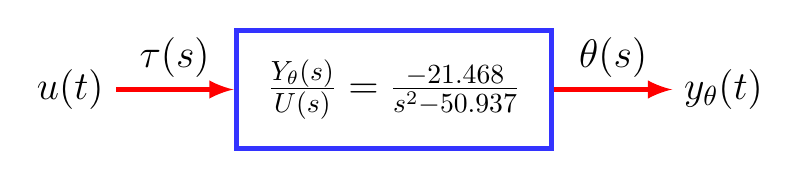
\begin{tikzpicture}
    % Box with the specified transfer function
    \node[draw, rectangle, minimum height=1.5cm, minimum width=4cm, thick, draw=blue!80, line width=2pt] (system)
    {\Large $\frac{Y_\theta (s)}{U(s)} = \frac{-21.468}{s^2 - 50.937}$};

    % Arrow for input u(t) pointing towards the system with black text and label \tau(s)
    \draw[<-, >=latex, red, line width=2pt] (system.west) -- ++(-1.5,0) node[above, midway, text=black] {\Large $\tau(s)$} node[left, text=black] {\Large $u(t)$};

    % Arrow for output y_\theta(t) exiting

from the system with black text
    \draw[->, >=latex, red, line width=2pt] (system.east) -- ++(1.5,0) node[above, midway, text=black] {\Large $\theta(s)$} node[right, text=black] {\Large $y_\theta(t)$};
\end{tikzpicture}



\vspace*{1cm}

\centering

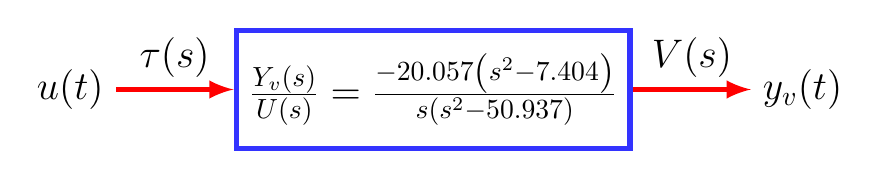
\begin{tikzpicture}
    % Single box with the combined transfer function
    \node[draw, rectangle, minimum height=1.5cm, minimum width=5cm, thick, draw=blue!80, line width=2pt] (system) 
    {\Large $\frac{Y_{v}(s)}{U(s)} = \frac{-20.057 \left(s^2 - 7.404\right)}{s \left(s^2 - 50.937\right)}$};

    % Arrow for input u(t) pointing towards the system with black text
    \draw[<-, >=latex, red, line width=2pt] (system.west) -- ++(-1.5,0) node[above, midway, text=black] {\Large $\tau(s)$} node[left, text=black] {\Large $u(t)$};

    % Arrow for output y(t) exiting from the system with black text
    \draw[->, >=latex, red, line width=2pt] (system.east) -- ++(1.5,0) node[above, midway, text=black] {\Large $V(s)$} node[right, text=black] {\Large $y_v(t)$};
\end{tikzpicture}

\caption[]{The Segway's transfer functions for the lean angle and cart speed are as given, where $u(t)$ is the motor torque. At the end of the Chapter, we will seek to control \textbf{simultaneously} these two key quantities. Can you see any special structure that may help us with that? }
\label{fig:SegwayTwoTransferFunctions}
\end{figure}


\vspace*{.2cm}
\begin{lstlisting}[language=Julia,style=mystyle]
using LinearAlgebra, Symbolics

# Set equilibirum Point
qe = [0.0;0]

F = dyn_mod_planarSegway(qe, 0*qe)
D = F.D; 
JacG = F.JacG; 
B = F.B; 

# build the linearized model about the given equilibrium point
A21 = -D\JacG; # A21 = cleanUp(A21); 
n, m = size(B)
A = [zeros(n,n) I(n); A21 zeros(n,n)];
b = [zeros(n,m); F.D \ B];
display(A)
display(b)

# Define the various outputs
c_th = [1.0 0 0 0]

# model params
g, m_wh, m_pend, L, r_wh, J_pend, J_wh, J_rotor, N = modelParameters() 

c_v1 = [0 0 0 r_wh]


# Define the symbolic variables and transfer functions
@Symbolics.variables s
G_th = c_th*inv(s*I(4) - A)*b
G_v1 = c_v1*inv(s*I(4) - A)*b

# Simplify
G_th = Symbolics.simplify(G_th[1])
println(G_th)

println(" ")

G_v1 = Symbolics.simplify(G_v1[1])
println(G_v1)
\end{lstlisting}
\textbf{Output} 
\begin{verbatim}
4×4 Matrix{Float64}:
    0.0      0.0  1.0  0.0
    0.0      0.0  0.0  1.0
   50.9373  -0.0  0.0  0.0
 -162.687   -0.0  0.0  0.0
 
4×1 Matrix{Float64}:
   0.0
   0.0
 -21.467741053946913
  80.22714380349518
  
-21.467741053946913 / (-50.93726022670157 + s^2)
 
(-148.50513185627278 + 20.056785950873795(s^2)) / (-50.93726022670157s + s^3)

\end{verbatim}

\Qed

\begin{factColor}{Factoring the Segway's Transfer Function}{FactorSegwayTF}

Because transfer functions are rational functions of the Laplace variable, $s$, the rules of ordinary algebra apply to them. While factoring an ODE seems far-fetched at best, expressing polynomials and rational functions in terms of factors is ordinary. Applying this idea to the Segway, its transfer function from motor torque to cart speed can be factored into two terms, as shown below. Indeed,  $\frac{-20.057}{-21.468} = 0.934$ to three significant digits, while the other terms are ``self-evident''. 

\begin{center}
    


\vspace*{1cm} 

\begin{tikzpicture}[auto, node distance=2cm, >=latex']
% We define the styles for the blocks and the arrows
 \tikzset{
block/.style = {draw, rectangle, thick, draw=blue!80, line width=2pt, minimum height=3em, minimum width=8em},
line/.style = {draw, -latex', thick, red, line width=2pt},
}

 % Motor torque block
 \node [block] (motor) {\Large $\bm{\frac{-21.468}{s^2 - 50.937 }}$ } ;
 \node [above of=motor, yshift=0.2cm, node distance=1cm] (motorlabel) {\textbf{\Large Orientation}};

 % Body orientation block
 \node [block, right of=motor, node distance=4.5cm] (body) { \Large $\bm{ {\frac{0.934 \, \left(s^2- 7.407\right)}{s} }$}};
 \node [above of=body, yshift=0.2cm, node distance=1cm] (bodylabel) {\textbf{\Large Speed}};

 % Arrows and labels for input and output
 \draw [line] ([xshift=-2cm]motor.west) -- (motor.west) node[midway, above, black] {\Large $\tau(s)$} node[at start, left, black] {\Large $u(t)$};
 \draw [line](motor.east) -- (body.west) node[midway, above, black] {\Large $\theta(s)$};
\draw [line] (body.east) -- ([xshift=2cm]body.east) node[midway, above, black] {\Large $V(s)$} node[at end, right, black] {\Large $y_v(t)$};


\end{tikzpicture}

\end{center}

\vspace*{1cm}
\textcolor{blue}{\bf \large The above factorization shows mathematically how the orientation of the Segway's body directly affects its speed, something that is much harder to see from the ODE itself. It suggests a two-pronged attack on how to control the Segway: first, stabilize the orientation and, second, use the orientation as a pseudo-actuator for the speed.}

\bigskip

\end{factColor}





\vspace*{.2cm}

\section{Poles, Zeros, and BIBO Stability}
\label{sec:PolesBIBO}

In Chapter~\ref{sec:ExponentialStabilityLTIodes}, we studied linear ODEs of the form $\dot{x} = Ax, ~~x(t_0) = x_0$, and learned that all solutions asymptotically converged to the origin if, and only if, the real parts of the eigenvalues of $A$ have negative real parts. \textcolor{blue}{\bf The main message of this section is that the roots of the denominator of a transfer function work just like eigenvalues: if their real parts are negative, then bounded input signals give rise to bounded output signals.} 

\subsection{Poles and Zeros}
A transfer function is {\bf rational} if it can be expressed as the ratio of two polynomials. 


\vspace*{.2cm}

\begin{tcolorbox}[colback=mylightblue, title = {\bf Poles and Zeros}, breakable]

\begin{definition} 
\label{def:PolesZeros}
For a rational transfer function $G(s)=\frac{N(s)}{D(s)}$, the polynomials $N(s)$ and $D(s)$ are said to be \textbf{coprime} if they have no common roots. In this case, the roots of $N(s)$ are the \textbf{zeros} of $G(s)$ and the roots of $D(s)$ are the \textbf{poles}. 

\end{definition}

\textbf{Note:} If $N(s)$ and $D(s)$ have common factors, hence yielding common roots, the common factors must be canceled before determining the zeros and poles of the transfer function.
\end{tcolorbox}

\vspace*{.2cm}


\begin{example}
\label{ex:OLPolesZeros}
Determine the zeros and poles of the transfer functions 
 \begin{enumerate}
\renewcommand{\labelenumi}{(\alph{enumi})}
\setlength{\itemsep}{.2cm}
\item $G_1(s) = \frac{2}{s^2-1}$

\item $G_2(s) = \frac{s+2}{s^2-1}$ 

\item $G_3(s) = \frac{s+1}{s^2-1}$

\item $G_4(s) = \frac{2s-4}{s^2+2s+2}$.
\end{enumerate}
\end{example}

\textbf{Solution:}
\begin{enumerate}
\renewcommand{\labelenumi}{(\alph{enumi})}
\setlength{\itemsep}{.2cm}

\item $N_1(s) = 2$ has no roots and $D_1(s) = s^2-1 = (s-1)(s+1)$ has roots $\pm 1$. $N_1(s)$ and $D_1(s)$ are therefore coprime; it follows that $G_1(s)$ has no zeros and two poles at $\pm1$.\\

\item $N_2(s)=s+2$ has one root $-2$ which is distinct from the roots of $D_2(s) = s^2-1$, which are $\pm 1$. Thus $N_2(s)$ and $D_2(s)$ are coprime and it follows that $G_2(s)$ has one zero at $-2$ and two poles at $\pm1$.\\

\item $N_3(s)=s+1$ has one root $-1$ which is also a root of $D_3(s)=s^2-1$. Thus $N_3(s)$ and $D_3(s)$ are \emph{not coprime}. To determine the zeros and poles of $G_3(s)$, the common factor of $(s+1)$ is removed, yielding
 $$G_3(s) = \frac{s+1}{(s+1)(s-1)} = \frac{1}{s-1}. $$
 It follows that $G_3(s)$ has no zeros and one pole at $1$.\\

\item  $N_4(s)=2(s-2)$ has a root at $2$, which is distinct from the roots of $D_4(s) = s^2 + 2s + 2 = (s+1+\im)(s+1-\im)$, which are $-1\pm \im$. $N_4(s)$ and $D_4(s)$ are therefore coprime; it follows that $G_4(s)$ has a zero at $2$ and two poles at $-1\pm \im$.

\end{enumerate}

\subsection{BIBO Stability}

We treated bounded functions way back in Chapter~\ref{sec:BoundedFunctions}. An \textbf{input or output signal} $s:[0, \infty) \to \real$ is \textbf{bounded} if there exists a constant $M$ such that $|s(t)|\le M$ for all $t\ge 0$. Hence, signals such as constants, $\sin(\omega t) \, \ustep(t)$, $\cos(\omega t) \, \ustep(t)$, $t^k \, e^{at} \ustep(t)$ for $a<0$, and products of such functions are bounded. Functions such as $e^{at} \ustep(t)$ and $t^k \, \ustep(t)$ for $a>0$ and $k>0$ are unbounded. 

\begin{tcolorbox}[colback=mylightblue, title = {\bf BIBO Stability}, breakable]

\begin{definition} 
\label{def:BIBOstable}
A system is \emph{bounded-input bounded-output} stable, or \textbf{BIBO stable} for short, if the output is bounded whenever the input is bounded. \\

If the system is \textbf{not} BIBO stable, it is said to be \textbf{unstable}.
\end{definition}

\textbf{Note:} To be extra clear, the word ``whenever'' here means the output must remain bounded for ``all possible'' bounded inputs, $u:[0, \infty) \to \real$. That sounds like it could be hard to check!
\end{tcolorbox}

\vspace*{.2cm}

Recall that a system is \textbf{causal} if present values of the output do not depend on future values of the input. If the system has a rational transfer function $G(s)$, then the system is causal if, and only if, the degree of the numerator is less than or equal to the degree of the denominator. \textbf{Transfer functions that satisfy this property have a special name; they are said to be} \textcolor{red}{\bf proper}.

\vspace*{.2cm}

\begin{propColor}{Poles and BIBO Stability}{PolesBIBOStability}
    A system with a proper rational transfer function is BIBO stable if, and only if, its poles have negative real parts. In other words, the stability of a rational transfer function
$$G(s)=\frac{N(s)}{D(s)},$$
is completely determined by its poles as long as the degree of the numerator polynomial is less than or equal to the degree of the denominator polynomial. \\

\textbf{Note:} The zeros do not play a role in stability.
\end{propColor}

\vspace*{.2cm}

\begin{figure}[hbt]

\begin{minipage}[h]{.46\linewidth}
   \centering
   \includegraphics[width=0.8\linewidth]{graphics/Chap10/UnstableRealPole.png}
\end{minipage}\hfill
\begin{minipage}[h]{.46\linewidth}
   \centering
  \includegraphics[width=0.8\linewidth]{graphics/Chap10/StepUnstableFirstOrder.png}
\end{minipage}

		
\begin{minipage}[h]{.46\linewidth}
   \centering
   \includegraphics[width=0.8\linewidth]{graphics/Chap10/StableRealPole.png}
\end{minipage}\hfill
\begin{minipage}[h]{.46\linewidth}
   \centering
  \includegraphics[width=0.8\linewidth]{graphics/Chap10/StepStableFirstOrder.png}
\end{minipage}

\caption{The positions of the poles are marked with a ${\mathlarger{ \bm{\times}}}\, $. For a positive real pole, bounded inputs can give rise to unbounded outputs, whereas for a negative real pole, bounded inputs always give rise to bounded outputs.}
	\label{fig:FiguresPolesZerosBIBO:StepResponseWithRealPole}
\end{figure}

\vspace*{.2cm}

To illustrate the connections between time-domain models, transfer functions, poles, and BIBO stability, consider a system represented by a first-order differential equation with input $u(t)$ and output $y(t)$,
$$ \dot{y}(t) - y(t) = u(t).$$
In the s-domain, the model becomes $s Y(s) - Y(s) = U(s)$, yielding
$$Y(s) = G(s) U(s),$$
where the transfer function is
$$G(s) = \frac{1}{s-1}.$$
The pole is $s=+1$, and thus the system is unstable. Is it easy to give a bounded input that results in an unbounded output? Absolutely.\\

For definiteness, suppose the input is a unit step, $\ustep(t)$. Then, from Table~\ref{tab:LaplaceTransformPairs}, $U(s) = \frac{1}{s}$ giving
$$Y(s) = \frac{1}{s-1} \frac{1}{s}.$$
Applying the method of partial fraction expansion,
$$Y(s) = -\frac{1}{s} + \frac{1}{s-1}.$$
Taking the inverse Laplace transform yields
\begin{equation}
\label{eqn:PolesZerosBIBO:FirstOrderOutputUnstable}
y(t) =\left(e^{t} -1\right) \ustep(t).
\end{equation}
From this equation, the output $y(t)$ is unbounded, diverging to infinity as $t$ goes to infinity, as shown in the upper half of Fig. \ref{fig:FiguresPolesZerosBIBO:StepResponseWithRealPole}.\\

On the other hand, for the model
$$ \dot{y}(t) + y(t) = u(t),$$
the transfer function is
$$G(s) = \frac{1}{s+1}.$$
The pole is $s=-1$, and hence the system is BIBO stable. Computing the output in response to a unit-step input gives
\begin{equation}
\label{eqn:PolesZerosBIBO:FirstOrderOutputStable}
y(t) = \left(1-e^{-t} \right) \ustep(t).
\end{equation}
From this equation, the output converges to 1.0 as $t$ goes to infinity, and, in particular, it is bounded for all $t\ge0$, as illustrated in the lower half of Fig. \ref{fig:FiguresPolesZerosBIBO:StepResponseWithRealPole}.


\vspace*{.2cm}
\begin{example}
\label{ex:BIBOstabilityOL}
    Determine the stability of the transfer functions 
\begin{enumerate}
\renewcommand{\labelenumi}{(\alph{enumi})}
\setlength{\itemsep}{.2cm}
\item $G_1(s) = \frac{2}{s^2-1}$

\item $G_2(s) = \frac{s+2}{s^2-1}$ 

\item $G_3(s) = \frac{s+1}{s^2-1}$

\item $G_4(s) = \frac{2s-4}{s^2+2s+2}$

\item  $G_5(s) = \frac{s-1}{s}$,
\end{enumerate}
where the first four transfer functions are taken from the previous example, and the last one is new.
\end{example}

\textbf{Solutions:} $G_1(s)$, $G_2(s)$ and $G_3(s)$ each has a pole at $+1$, and thus they are unstable. The  poles of $G_4(s)$ are $-1\pm \im$, which have negative real parts, and hence the transfer funciton is BIBO stable. $G_5(s)$ has a pole at the origin, and hence it is unstable. 
\Qed

\vspace*{.2cm}
\begin{center}
\setlength{\fboxrule}{2pt}  % Setting the thickness of the border line
   \fbox{ \parbox{0.9\linewidth}{
   \bigskip    
   \textcolor{blue}{\large \bf At this point, the role of zeros seems somewhat mysterious. The zeros will come into the picture when closed-loop systems are analyzed.}\\
}
} 
\end{center}
\vspace*{.2cm}


\begin{example}(Optional Read:) If a rational transfer function is not proper, do the poles still determine its stability? The short answer is no.
    
\end{example}
\textbf{Solution:}
 If you are curious as to why not, consider $G(s) = s$, which corresponds to a differentiator, that is, the system
$$y(t) = \frac{d u(t)}{dt},$$
where $u(t)$ is the input. The input $\sin(t^2)$ is bounded, since it takes values between $-1$ and $1$, but the corresponding output $y(t) = 2 t \cos(t^2)$ is unbounded. \\

The hardcore among you may think that the transfer function has no poles, and therefore, it is untrue that all of its poles have negative real parts. Instead of arguing semantics, consider the transfer function,
\begin{align*}
G(s) &= G_a(s) + G_b(s) \\
& = s + \frac{1}{s+2} \\
& = \frac{s(s+2)}{s+2} + \frac{1}{s+2} \\
& = \frac{s^2+2s+1}{s+2},
\end{align*}
which is improper. A quick calculation shows that it has two zeros at $-1$ and a pole at $-2$. But the system is not BIBO stable because the bounded input $u(t) = \sin(t^2)$ produces the output
$$ y(t) = y_a(t) + y_b(t),$$
where $y_a(t) = 2 t \cos(t^2)$, which is unbounded, and the second term, being the output of a system with BIBO stable transfer function $G_b(s)$, must be bounded. The sum of an unbounded signal and a bounded signal is unbounded. Thus, a bounded input has produced an unbounded output, showing the system is unstable.
\Qed

\vspace*{.2cm}

\begin{figure}[hbt]
      \centering
      %%\includegraphics[width = .5\linewidth]{graphics/Chap10/CLSystem_G.png}
      \begin{tikzpicture}[>=Latex, thick, line/.style={draw=red, line width=2pt}, border/.style={draw=blue!80, line width=2pt}, scale=1.5, every node/.style={scale=1.25}]
    % Define styles for blocks, sum nodes, input and output
    \tikzstyle{block} = [draw, fill=white, rectangle, minimum height=3em, minimum width=5em, border=1pt]
    \tikzstyle{sum} = [draw, fill=white, circle, node distance=2cm, border=1pt]
    \tikzstyle{input} = [coordinate]
    \tikzstyle{output} = [coordinate]

    % Nodes placement
    \node [input, name=input] {};
    \node [sum, right of=input, node distance=2.4cm] (sum) {\(\Sigma\)};
    \node [block, right of=sum, node distance=2.6cm] (system) {$G(s)$}; % Combined block for G(s)
    \node [output, right of=system, node distance=2.9cm] (output) {};

    % Draw edges
    \draw[line=2pt,->] (input) -- node[above] {$R(s)$} (sum);
    \draw[line=2pt,->] (sum) -- node[above] {$E(s)$} (system);
    \draw[line=2pt] (system) -- ++(1.5,0) coordinate (feedbackPoint); % Extend line to the right for feedback
    \draw[line=2pt,->] (system) -- node[above] {$Y(s)$} (output); % Continue to output

    % Creating the feedback loop
    \draw[line=2pt] (feedbackPoint) |- ($(sum)!0.5!(system)-(0,1cm)$);
    \draw[line=2pt,->] ($(sum)!0.5!(system)-(0,1cm)$) -| node[pos=0.99, right] {$ $} (sum.south);

    % Adding labels above the sum node and the system block
    \node [above=of sum, yshift=0.2cm] (summerLabel) {\textbf{Summer}}; % Adjust the yshift for desired distance
    \node [above=of system, yshift=0.05cm] (forwardPathLabel) {\textbf{Forward Path}}; % Adjust the yshift for desired distance


    % Labeling the sum block
    \draw (sum.west) ++(-0.15,-0.3) node {$+$};
    \draw (sum.south) ++(0.25,-0.1) node {$-$};
\end{tikzpicture}
    \caption[]{Unity negative feedback system.}
    \label{fig:UnityFeedbackSystems:StandardUnityFeedabckSystem}
  \end{figure}

%\section{Closed-loop Transfer Functions and Test Functions}
\section{Unity Feedback Systems}

A common control system configuration, and the easiest one to study when first learning the subject of feedback control, is the \textbf{unity feedback system} shown in Fig.~\ref{fig:UnityFeedbackSystems:StandardUnityFeedabckSystem}. It is also called a \textbf{negative feedback system} due to the minus sign on the feedback loop at the summer. In this figure, $Y(s)$ is the system output, $R(s)$ is the reference command, and $E(s)$ is the error between the output and the reference.  The reference command $R(s)$ normally specifies the desired output of the system. When the reference command is a constant, the reference value is also called a \textbf{setpoint}. The transfer function in the \textbf{forward path} is $G(s)$, whereas the transfer function in the \textbf{feedback path} (the bottom loop) is one, the source of the name, \textbf{unity} feedback system.

\subsection{Closed-loop Transfer Functions}
\label{sec:UnityFeedbackSystems:cltf}

The block diagram in Fig.~\ref{fig:UnityFeedbackSystems:StandardUnityFeedabckSystem} is equivalent to the following set of linear equations
\begin{eqnarray}
\label{eqn:UnityFeedbackSystems:StandardUnityFeedabckSystem}
  E(s) &=& R(s) - Y(s) \\
  Y(s) &=& G(s) E(s).
\end{eqnarray}
Solving these two equations for $Y(s)$ as a function of $R(s)$ results in
\begin{align*}
  Y(s) &= G(s)( R(s) - Y(s) ) \\
       & = G(s)R(s) - G(s)Y(s),
       \end{align*}
  and thus
$$
 Y(s) + G(s)Y(s) = G(s)R(s),$$
 which is equivalent to
$$  (1 + G(s))Y(s) = G(s)R(s).$$
Hence
\begin{empheq}[box=\bluebox]{equation}
 Y(s) = \frac{G(s)}{1 + G(s)}R(s),
\label{eqn:UnityFeedbackSystems:R2Y}
\end{empheq}
from which it follows that the transfer function from $R(s)$ to $Y(s)$ is
\begin{empheq}[box=\bluebox]{equation}
 \frac{Y(s)}{R(s)} = \frac{G(s)}{1 + G(s)}.
\label{eqn:UnityFeedbackSystems:R2Yb}
\end{empheq}

The same steps can be repeated to determine the transfer function from $R(s)$ to $E(s)$,
$$E(s) = R(s) - G(s)E(s)$$
and $$(1+G(s)) E(s) = R(s).$$

Thus,
\begin{empheq}[box=\bluebox]{equation}
 E(s) = \frac{1}{1 + G(s)}R(s),
\label{eqn:UnityFeedbackSystems:R2E}
\end{empheq}
which yields the transfer function as
\begin{empheq}[box=\bluebox]{equation}
 \frac{E(s)}{R(s)} = \frac{1}{1 + G(s)}.
\label{eqn:UnityFeedbackSystems:R2Eb}
\end{empheq}

\vspace*{.2cm}
\begin{example} 
\label{ex:ClosedLoopPoles}
For the unity feedback system in Fig.~\ref{fig:UnityFeedbackSystems:StandardUnityFeedabckSystem}, compute the poles of $\frac{Y(s)}{R(s)}$ and $\frac{E(s)}{R(s)}$ for each of the following forward-path transfer functions,
 \begin{enumerate}
\renewcommand{\labelenumi}{(\alph{enumi})}
\setlength{\itemsep}{.2cm}
\item $G_1(s) = \frac{2}{s^2-1}$

\item $G_2(s) = \frac{s+2}{s^2-1}$ 

\item $G_3(s) = \frac{s+1}{s^2-1}$.
\end{enumerate}
    
\end{example}
\textbf{Solutions:} Before starting the solutions, suppose you had the following ratio of rational numbers
$$ \frac{\frac{3}{4}}{1 + \frac{3}{4}},$$
and you wanted to reduce it to a standard ratio of two integers. You would be unlikely to find the problem intimidating because you know how to clear the denominator as follows,
\begin{align*}
\frac{\frac{3}{4}}{1 + \frac{3}{4}} & = \frac{3}{4 + 3}~~(\text{multiply top and bottom by}~~4)\\
& = \frac{3}{7}.
\end{align*}
Because there are no common factors, this is the final answer. If you somehow arrived at $\frac{6}{14}$, you would remove the common factor of two (aka, 6 and 14 are not \href{https://en.wikipedia.org/wiki/Coprime_integers}{coprime}). We are going to do the same for rational functions. \textbf{What is mindbogglingly cool is that these rational functions are transfer functions and, THEREFORE, correspond to ODEs!} Never in a million years would you have imagined manipulating derivatives like this. Laplace was a genius.\\ 

 \begin{enumerate}
\renewcommand{\labelenumi}{(\alph{enumi})}
\setlength{\itemsep}{.2cm}
\item $G_1(s) = \frac{2}{s^2-1}$ \quad \Ans Poles of $\frac{Y(s)}{R(s)}$ and $\frac{E(s)}{R(s)}$ are the same and equal $\pm \im$. Hence, the closed-loop system is not BIBO stable.\\

\begin{align*}
    \frac{Y(s)}{R(s)} & = \frac{G_1(s)}{1 + G_1(s)} \\
    & =  \frac{\frac{2}{s^2-1}}{1 + \frac{2}{s^2-1}}~~ (\text{multiply top and bottom by}~~(s^2-1))\\
    & = \frac{2}{(s^2-1) + 2} \\
    & = \frac{2}{s^2+1}.
\end{align*}
Hence, the poles are $\pm \im$. We did not have to worry about a common factor because the numerator is a constant and has no roots. In a similar fashion, we compute
\begin{align*}
    \frac{E(s)}{R(s)} & = \frac{1}{1 + G_1(s)} \\
    & =  \frac{1}{1 + \frac{2}{s^2-1}}~~ (\text{multiply top and bottom by}~~(s^2-1))\\
    & = \frac{2(s^2-1)}{(s^2-1) + 2} \\
    & = \frac{2(s^2 - 1)}{s^2+1}.
\end{align*}
The numerator has roots $\pm 1$, while the denominator has roots $\pm \im$. There are no common factors and hence the poles are $\pm \im.$

\item $G_2(s) = \frac{s+2}{s^2-1}$ \quad \Ans Poles of $\frac{Y(s)}{R(s)}$ and $\frac{E(s)}{R(s)}$ are the same and equal $-\frac{1}{2} \pm \im \frac{\sqrt{3}}{2}$. Hence, the closed-loop system is BIBO stable.\\

\begin{align*}
    \frac{Y(s)}{R(s)} & = \frac{G_2(s)}{1 + G_2(s)} \\
    & =  \frac{\frac{s+2}{s^2-1}}{1 + \frac{s+2}{s^2-1}}~~ (\text{multiply top and bottom by}~~(s^2-1))\\
    & = \frac{s+2}{(s^2-1) + (s+2)} \\
    & = \frac{s+2}{s^2+s +1}.
\end{align*}
The root of the numerator is $-2$ and the roots of the denominator are $-\frac{1}{2} \pm \im \frac{\sqrt{3}}{2}$.  Because there are no common factors, the poles are $-\frac{1}{2} \pm \im \frac{\sqrt{3}}{2}$. In a similar fashion, we compute
\begin{align*}
    \frac{E(s)}{R(s)} & = \frac{1}{1 + G_2(s)} \\
    & =  \frac{1}{1 + \frac{s+2}{s^2-1}}~~ (\text{multiply top and bottom by}~~(s^2-1))\\
    & = \frac{(s^2-1)}{(s^2-1) +(s+ 2)} \\
    & = \frac{(s^2 - 1)}{s^2+s + 1}.
\end{align*}
The numerator has roots $\pm 1$, while the denominator has roots $-\frac{1}{2} \pm \im \frac{\sqrt{3}}{2}$. There are no common factors and hence the poles are $-\frac{1}{2} \pm \im \frac{\sqrt{3}}{2}$.

\item $G_3(s) = \frac{s+1}{s^2-1}$ \quad \Ans The pole of $\frac{Y(s)}{R(s)}$ and $\frac{E(s)}{R(s)}$ is the same and equals $s=0$. Hence, the closed-loop system is not BIBO stable.\\

\begin{align*}
    \frac{Y(s)}{R(s)} & = \frac{G_3(s)}{1 + G_3(s)} \\
    & =  \frac{\frac{s+1}{s^2-1}}{1 + \frac{s+1}{s^2-1}}~~ (\text{multiply top and bottom by}~~(s^2-1))\\
    & = \frac{s+1}{(s^2-1) + (s+1)} \\
    & = \frac{s+1}{s^2+s } \\
    & = \frac{s+1}{s (s+1) } \\
    & = \frac{1}{s}
\end{align*}
The numerator has no roots (because we saw the cancellation and took care of it) and the root of the denominator is  $0$.  Because there are no common factors, the pole is $s=0$. In a similar fashion, we compute
\begin{align*}
    \frac{E(s)}{R(s)} & = \frac{1}{1 + G_3(s)} \\
    & =  \frac{1}{1 + \frac{s+1}{s^2-1}}~~ (\text{multiply top and bottom by}~~(s^2-1))\\
    & = \frac{(s^2-1)}{(s^2-1) +(s+ 1)} \\
    & = \frac{(s^2 - 1)}{s^2+s} \\
    & =  \frac{(s+1)(s-1)}{s(s+1)}\\
    & = \frac{s-1}{s}.
\end{align*}
The numerator has a root at $+1$, while the denominator has a root at  $0$. There are no common factors and hence the pole is $s=0$.
\end{enumerate}

\textbf{Note:} The common factor in the numerator and denominator can be traced back to the common factor in the open-loop transfer function,
$$G_3(s) = \frac{s+1}{s^2-1} = \frac{s+1}{(s-1)(s+1)}.$$
If the common factor had been removed BEFORE computing the closed-loop transfer functions, the resulting polynomials would not have had a common factor; that is, they, too, would have been coprime. As part of feedback design, we sometimes like to cancel a ``STABLE zero'' by a ``STABLE pole''. We'll come back to this point later. 
\Qed

\bigskip
We deliberately went through every step in each problem to underline the repetitive nature of the computations. 

\bigskip

\begin{propColor}{Closed-Loop Transfer Functions}{CLTF}
Suppose that $G(s)=\frac{N(s)}{D(s)}$ is the forward-path transfer function for the unity feedback system in Fig.~\ref{fig:UnityFeedbackSystems:StandardUnityFeedabckSystem}. Then, the closed-loop transfer functions are
\begin{equation}
    \begin{aligned}
        \frac{Y(s)}{R(s)} & = \frac{N(s)}{D(s) + N(s)} \\[1em]
        \frac{E(s)}{R(s)} & = \frac{D(s)}{D(s) + N(s)}.
    \end{aligned}
\end{equation}
Moreover, if $N(s)$ and $D(s)$ are coprime, then so are the numerators and denominators of $ \frac{Y(s)}{R(s)}$ and $ \frac{E(s)}{R(s)}$.    
\end{propColor}

\textbf{Proof:} Simple calculations show that the two transfer functions associated with a unity feedback system are as stated. Indeed, 
$$
 \frac{Y(s)}{R(s)} = \frac{\frac{N(s)}{D(s)}}{1 + \frac{N(s)}{D(s)}} =  \frac{N(s)}{D(s) + N(s)},
$$
and
$$
 \frac{E(s)}{R(s)} = \frac{1}{1 + \frac{N(s)}{D(s)}} =  \frac{D(s)}{D(s) + N(s)}.
$$
In each case, the numerator and denominator have been multiplied by $D(s)$ to simplify the expressions to a ratio of polynomials.\\

Next, we show that if $N(s)$ and $D(s)$ are coprime (no common roots), then the polynomials $N(s)$ and $D(s) + N(s)$ are coprime as well. To show this, suppose that $s_1$ is a root of $N(s)$, that is, $N(s_1)=0$. Can it also be a root of $D(s) + N(s)$? The answer is no, because if $N(s_1)=0$, then $D(s_1) + N(s_1)= D(s_1)$. Hence, if  $D(s_1) + N(s_1)=0$, then $D(s_1)=0$, which shows that $s_1$ would then have to be a root of $D(s)$, which is not possible due to $N(s)$ and $D(s)$ being coprime. The identical argument applies to the second transfer function as well.
\Qed.

\subsection{Closed-loop Poles and Zeros}

\bigskip
Proposition~\ref{thm:CLTF} puts us in a positon to define the closed-loop poles and zeros of a unity feedback system.
\bigskip

\vspace*{.2cm}

\begin{tcolorbox}[colback=mylightblue, title = {\bf Closed-Loop Poles and Zeros}, breakable]

\begin{definition} 
\label{def:ClosedLoopPolesZeros}
For the unity feedback system in Fig.~\ref{fig:UnityFeedbackSystems:StandardUnityFeedabckSystem}, with forward-path transfer function $G(s) = \frac{N(s)}{D(s)}$ coprime, the \textbf{closed-loop poles} are the roots of $D(s) + N(s)$ and the \textbf{closed-loop zeros} are the roots of $N(s)$. It follows that the zeros of the forward-path transfer function are also the closed-loop zeros of the corresponding unity feedback loop
\end{definition}

\textbf{Notes:} (a) If $N(s)$ and $D(s)$ have common factors, hence yielding common roots, the common factors must be canceled before determining the zeros and poles of the closed-loop system. (b) 
Because we are normally interested in shaping the transient response of the transfer function from reference command to output, the zeros of interest to us are those of $ \frac{Y(s)}{R(s)}$.
\end{tcolorbox}

\vspace*{.2cm}

Even though it is a slight abuse of terminology, the zeros of $G(s)$ are often called the open-loop zeros, and the poles of $G(s)$ are often called the open-loop poles. This terminology makes sense because if one \emph{opens the loop} by disconnecting the feedback path from the summer in Fig.~\ref{fig:UnityFeedbackSystems:StandardUnityFeedabckSystem}, the transfer function from $R(s)$ to $Y(s)$ is $G(s)$.

\vspace*{.2cm}
\begin{example} Give the open-loop (OL) and closed-loop (CL) poles and zeros for the forward-path (FP) transfer functions taken from Example~\ref{ex:ClosedLoopPoles}.
 \begin{enumerate}
\renewcommand{\labelenumi}{(\alph{enumi})}
\setlength{\itemsep}{.2cm}
\item $G_1(s) = \frac{2}{s^2-1}$

\item $G_2(s) = \frac{s+2}{s^2-1}$ 

\item $G_3(s) = \frac{s+1}{s^2-1}$.
\end{enumerate}    
\end{example}
\textbf{Solutions:}
Most of the work has been done in Examples~\ref{ex:OLPolesZeros}, \ref{ex:BIBOstabilityOL}, and \ref{ex:ClosedLoopPoles}. The purpose here is to collect it all together and practice the new vocabulary.\\

\begin{center}
\renewcommand{\arraystretch}{1.5}
\begin{tabular}{|c|c|c|c|c|}
\hline
FP $G(s)$ & OL Zeros & OL Poles & CL Zeros & CL Poles \\ \hline
$\frac{2}{s^2-1} $    &   None       &   $\pm 1$       &    None      &    $\pm \im$      \\ \hline
$\frac{s+2}{s^2-1}$   &     $-2$     &   $\pm 1$        &     $-2$     &     $-\frac{1}{2} \pm \im \frac{\sqrt{3}}{2}$     \\ \hline
$\frac{s+1}{s^2-1}$      &   None       &   $+1$       &     None     &     $0$     \\ \hline
\end{tabular}
\end{center}
When there are no open-loop zeros, there are no closed-loop zeros. Because the numerator and denominator of $G_3(s)$ are not coprime, we had to first remove their common factor of $(s+1)$ before completing the table. 

\Qed

\begin{figure}[bt]
      \centering
      \begin{tikzpicture}[>=Latex, thick, line/.style={draw=red, line width=#1}, border/.style={draw=blue!80, line width=2pt}, scale=1.5, every node/.style={scale=1.25}]
    % Define styles for blocks, sum nodes, input and output
    \tikzstyle{block} = [draw, fill=white, rectangle, minimum height=3em, minimum width=5em, border=1pt]
    \tikzstyle{sum} = [draw, fill=white, circle, node distance=2cm, border=1pt]
    \tikzstyle{input} = [coordinate]
    \tikzstyle{output} = [coordinate]

    % Nodes placement
    \node [input, name=input] {};
    \node [sum, right of=input, node distance=2.4cm] (sum) {\(\Sigma\)};
    \node [block, right of=sum, node distance=2.6cm] (controller) {$C(s)$};
    \node [block, right of=controller, node distance=2.9cm] (system) {$P(s)$};
    \node [output, right of=system, node distance=2.4cm] (output) {};

    % Draw edges
    \draw[line=2pt,->] (input) -- node[above] {$R(s)$} (sum);
    \draw[line=2pt,->] (sum) -- node[above] {$E(s)$} (controller);
    \draw[line=2pt,->] (controller) -- node[above] {$U(s)$} (system);
    \draw[line=2pt] (system) -- ++(1.5,0) coordinate (feedbackPoint); % Extend line to the right for feedback
    \draw[line=2pt,->] (system) -- node[above] {$Y(s)$} (output); % Continue to output

    % Creating a new feedback loop without the Y(s) block
    \draw[line=2pt] (feedbackPoint) |- ($(sum)!0.5!(controller)-(0,1cm)$);
    \draw[line=2pt,->] ($(sum)!0.5!(controller)-(0,1cm)$) -| node[pos=0.99, right] {$ $} (sum.south);
    
    \node [above of=controller, yshift=0.2cm,  xshift=-0.3cm, node distance=1cm] (controllerlabel) {\textbf{\Large Compensator}};
    \node [above of=system, yshift=0.2cm, node distance=1cm] (systemlabel) {\textbf{\Large Plant}};
    \node [above of=input, yshift=0.2cm, xshift=0.7cm, node distance=1cm] (inputlabel) {\textbf{\Large Reference}};
    \node [above of=output, yshift=0.2cm, xshift=-0.4cm, node distance=1cm] (outputlabel) {\textbf{\Large Output}};

    
    % Labeling the sum block
    \draw (sum.west) ++(-0.15,-0.3) node {$+$};
    \draw (sum.south) ++(0.25,-0.1) node {$-$};
\end{tikzpicture}
    \caption[]{Cascade control system configuration, where $C(s)$ is the transfer function of the compensator and $P(s)$ is the transfer function of the plant. Their product, $G(s) = C(s)\, P(s)$ is the overall forward-path transfer function.}
    \label{fig:UnityFeedbackSystems:UnityC(s)P(s)}
  \end{figure}

\section{Cascade Control Architecture}
\label{sec:UnityFeedbackSystems:cascade}

  Figure~\ref{fig:UnityFeedbackSystems:UnityC(s)P(s)} is a refinement of the unity feedback system, where the forward path is written as a \textbf{cascade} connection of a \textbf{compensator} $C(s)$ and \textbf{plant} $P(s)$. Recall that ``plant'' is the generic term for the system that is to be controlled. The input to the plant is denoted $U(s)$. The plant input is the means by which the plant output is changed. For the Segway, the plant input was the torque at the wheels provided by the motors, while for the RLC circuit, it was the applied voltage.

The compensator is the algorithm that determines how to vary the input to the plant to regulate the plant output. In the cascade control configuration of Fig.~\ref{fig:UnityFeedbackSystems:UnityC(s)P(s)}, the compensator acts on $E(s):=R(s) - Y(s)$, the \textbf{error} between the reference command $R(s)$ and the measured output $Y(s)$, to produce the control input by
\begin{equation}
    U(s) = C(s) E(s).
\end{equation}
When the error is zero, the plant output is exactly following or \textbf{tracking} the reference command. One way to think of the compensator is that it attempts to adjust the plant input so that the plant output tracks the reference command. Equivalently, the compensator seeks to drive the error between the reference and output signals to zero.

The closed-loop transfer functions, \eqref{eqn:UnityFeedbackSystems:R2Yb} and \eqref{eqn:UnityFeedbackSystems:R2Eb} in Chapter~\ref{sec:UnityFeedbackSystems:cltf} easily updated to this new situation by indenifying $G(s):=C(s) P(s)$. Doing so yields,
\begin{empheq}[box=\bluebox]{equation}
 \frac{Y(s)}{R(s)} =\frac{C(s)P(s)}{1+C(s)P(s)}
\label{eqn:UnityFeedbackSystems:R2Y:Cascade}
\end{empheq}
and
\begin{empheq}[box=\bluebox]{equation}
 \frac{E(s)}{R(s)} =\frac{1}{1+C(s)P(s)}.
\label{eqn:UnityFeedbackSystems:R2E:Cascade}
\end{empheq}
Because $U(s)=C(s)E(s)$, it follows that
\begin{empheq}[box=\bluebox]{equation}
 \frac{U(s)}{R(s)} =\frac{C(s)}{1+C(s)P(s)}.
\label{eqn:UnityFeedbackSystems:R2U:Cascade}
\end{empheq}
All three of these transfer functions become important in most control system designs. 

\subsection{Two Common Compensators: Proportional (P) and Proportional-Derivative (PD)}
\label{sec:feedback:CommonCompensators}

We introduce here the two most commonly used compensators. A more complete list is available in Appendix~\ref{chap:AppFeedbackControlDesign}. 

\subsubsection{Proportional compensator}

\begin{equation}
\label{eq:PropCompensator}
C(s) = K_P,
\end{equation}
where $K_P$ is called a \textbf{proportional gain}. With a proportional compensator, the control signal is given by
$$ u(t) = K_P e(t) = K_P(r(t) - y(t)).$$
Adjusting $K_P$ allows the control signal to react more or less ``vigorously'' to the error between the commanded value of the output (aka, reference signal), $r(t)$, and the measured value of the output, $y(t)$. It adds neither zeros nor poles to the forward path of the feedback loop. For a first-order plant, $P(s)$, gain adjustment alone can achieve stability, as we illustrate next.\\

\begin{example} {\bf (Proportional feedback applied to an unstable first-order plant)}
Suppose the plant has transfer function $P(s)=\frac{1}{s-1}$ and the compensator is a \emph{proportional feedback} $C(s) = K_P$, where $K_P$ is a gain to be chosen. Determine the closed-loop transfer function $\frac{Y(s)}{R(s)}$ and evaluate its BIBO stability as a function of $K_P$.
\end{example}

\solution

  \begin{align*}
  \frac{Y(s)}{R(s)} &= \frac{C(s)P(s)}{1+C(s)P(s)}\\[1em]
    & = \frac{K_P \frac{1}{s-1}}{1+K_P \frac{1}{s-1} }~~ \left(\text{multiply top and bottom by}~~ (s-1)\right) \\[1em]
     & = \frac{K_P}{s-1+K_P}.
\end{align*}
The pole of the transfer function is the root of the denominator polynomial, $s-1+K_P=0$, yielding a single pole $1-K_P$. The closed-loop system is, therefore, BIBO stable if, and only if,  $K_P>1$.
\Qed

\bigskip
Feedback control design would be way too easy if we could stabilize all plants with proportional feedback! The following result will make it easier to show a limitation of proportional feedback control.\\

\begin{factColor}{Simplified Stability Test}{SimplifiedStabilityTest}
For real numbers $a_1$ and $a_0$, the roots of the quadratic equation
\begin{equation}
\label{eqn:UnityFeedbackSystems:QuadraticEqn}
 s^2 + a_1 s + a_0=0
 \end{equation}
have negative real parts if, and only if, $a_1>0$ and $a_0>0$. \\

\textbf{Note:} To apply the above result to 
$ \bar{a}_2 s^2 + \bar{a}_1 s + \bar{a}_0=0$, with $\bar{a}_2\neq 0$, you simply divide through by $\bar{a}_2$, yielding $a_1 = \frac{\bar{a}_1}{\bar{a}_2}$ and $a_0 = \frac{\bar{a}_0}{\bar{a}_2}$.
\end{factColor}

For a cubic equation, the result is, for real numbers $a_2$, $a_1$, and $a_0$, the roots of the equation
% \begin{equation}
% \label{eqn:UnityFeedbackSystems:CubicEqn}
$$
 s^3 + a_2 s^2 + a_1 s + a_0=0
 $$
 % \end{equation}
have negative real parts if, and only if, $a_2>0$, $a_0>0$, and $a_1 - \frac{a_0}{a_2} >0$. Similar results can be given for polynomials of arbitrary degree. The computations are typically organized in a table called the \href{https://en.wikipedia.org/wiki/Routh%E2%80%93Hurwitz_stability_criterion#:~:text=of%20degree%202.-,Routh%E2%80%93Hurwitz%20criterion%20for%20second%2C%20third%20and%20fourth%2Dorder%20polynomials,-%5Bedit%5D}{Routh array}, which is typically covered in Michigan's EECS 460 Control Systems Analysis and Design.

\bigskip
\begin{example} {\bf (Proportional feedback applied to an unstable second-order plant)}
Suppose the plant is instead $P(s)=\frac{1}{s(s-2)}$, with the previous proportional feedback, $C(s) = K_P$. Determine the transfer function $\frac{Y(s)}{R(s)}$ and evaluate its stability as a function of $K_P$.
\end{example}

\solution
Evaluating the closed-loop transfer function gives
    $$ \frac{Y(s)}{R(s)} = \frac{K_P}{s^2 -2s + K_P}.$$
    The poles of the transfer function are the roots of the polynomial $s^2-2s+K_P=0$. Applying the result of Fact~\ref{thm:SimplifiedStabilityTest}, it is seen that the coefficient $a_1 = -2 <0$ is independent of the value of the gain $K_P$, and hence at least one root will have a non-negative real part no matter the value of $K_P$. The closed-loop system is, therefore, unstable for all values of the gain $K_P$, and \textbf{something more sophisticated than proportional feedback is required to stabilize the closed-loop system}.
\Qed


\subsubsection{PD or Proportional-Derivative compensator}
\begin{equation}
\label{eq:PDcompensator}
   C(s) = K_P + K_D s = K_D \left(s + \frac{K_P}{K_D}\right) 
\end{equation}
has two gains, the proportional gain, $K_P$, which acts as before, and the \textbf{derivative gain}, $K_D$.  With a proportional-derivative (PD) compensator, the control signal is given by
$$ u(t) = K_P e(t) + K_D \dot{e}(t) = K_P(r(t) - y(t)) + K_D( \dot{r}(t) -  \dot{y}(t)).$$
The derivative term allows the controller to react with ``anticipation'' to changes in the error signal. Whoa! Does the controller become a psychic? Not exactly. If we approximate the derivative as
$$ \dot{e}(t) \approx \frac{e(t+ \delta t) - e(t)}{\delta t},$$
the control signal approximately depends on the error term at the future time, $t+ \delta t$, giving it a head start on making a correction to the closed-loop system. Another way to look at it is that the linear approximation of the error signal at a point $t_0$ is
$$ e(t) \approx e(t_0) + \underbrace{\frac{de(t_0)}{dt}}_{\dot{e}(t_0)}(t-t_0),$$
showing again that the derivative of $e$ allows the prediction of future values of the error signal over small intervals of time. This discussion is meant to provide intuition, so if it seems hand-wavy or confusing to you, just ignore it. The Laplace transform will soon clear up lingering doubts.\\

A PD compensator adds a zero in the forward path at $-\frac{K_P}{K_D}$, but has no poles. The derivative action of a PD compensator will prove useful for stabilizing a system and for reducing oscillations.\\

\begin{example} {\bf (PD compensation applied to an unstable second-order plant)}
Suppose the plant is $P(s)=\frac{1}{s(s-2)}$ and $C(s) = K_P + K_Ds$. Determine the transfer function $\frac{Y(s)}{R(s)}$ and evaluate its stability as a function of the controller gains.
\end{example}

\solution
Evaluating the closed-loop transfer function gives
    $$ \frac{Y(s)}{R(s)} = \frac{K_P + K_Ds}{(s^2 -2s) + (K_P + K_D s)} =  \frac{K_P + K_Ds}{s^2 + (K_D-2)s + K_P}.$$
    The poles of the transfer function are the roots of the polynomial $s^2 + (K_D-2)s + K_P=0$. After identifying the coefficients $a_1 = (K_D-2)$ and $a_0= K_P$, Fact~\ref{thm:SimplifiedStabilityTest} yields that the closed-loop system's poles have negative real parts if, and only if, $K_P>0$ and $K_D > 2$.    
\Qed

Is stability all we care about in a feedback loop? Hardly. We'll next look at the steady-state error, that is, the long-term ``accuracy'' of the control system. 

\subsection{Steady-State Error}
\label{sec:SSError:SystemType}

The \textbf{steady-state error}, or $\bm{e_{\rm SS}}$, is the asymptotic\footnote{That is, its value as $t \to \infty$.} value of the error signal defined in Figures \ref{fig:UnityFeedbackSystems:StandardUnityFeedabckSystem} and \ref{fig:UnityFeedbackSystems:UnityC(s)P(s)}. The steady-state error depends on the reference command and the forward-path transfer function. The expression for the error signal was derived in \eqref{eqn:UnityFeedbackSystems:R2E} and \eqref{eqn:UnityFeedbackSystems:R2E:Cascade}. When $e_{\rm SS}$ is small, the control system is accurately tracking the reference command as the system reaches a steady state. What happens between the closed-loop system being ``excited'' by an input signal and its reaching a steady state is called its transient response; this will be the subject of a separate section.

While the term ``steady-state'' can be defined for a range of reference signals, we will focus on the most common one, the unit-step function, that is, $R(s) = \frac{1}{s}$. Appendix~\ref{chap:AppFeedbackControlDesign} also looks at steady-state error for ramp inputs.\\

\begin{propColor}{Steady-State Error for Step Inputs Applied to BIBO Stable Closed-Loop Systems}{ESS} Assume the forward path transfer function is $G(s) = \frac{N(s)}{D(s)}$ and the closed-loop system is BIBO stable. Then the steady-state error for a unit-step command is well-defined and is given by
\begin{equation}
\label{eqn:SSError:SSE:stepb}
\bm{e_{SS} =\lim_{s \to 0} \frac{D(s)} {D(s) + N(s)}}.
\end{equation}
Moreover, if $G(s)$ does not have a pole at the origin, then
$$e_{SS} =\frac{D(0)}{D(0) + N(0)}\not = 0,$$
while if $G(s)$ has one or more poles at the origin, then $D(0)=0$ and the steady-state error is 
$$e_{SS} = 0.$$


\textbf{Note:} To be clear, the result also holds for $G(s) = C(s) P(s)$ arising from a Cascade Controller Architecture. \\
 

\textbf{Note:} What happens to $e_{SS}$ if the reference is $r(t) = r_0 \cdot \ustep(t)$, a scaled unit-step? Because $E(s) = \frac{1}{1 + G(s)} R(s)$, it follows that if the reference is scaled by $r_0$, then so is the error. Hence, $e_{SS}$ gives the \textit{relative error}, or, said another way, the \textit{percent error} in the output is $100\, e_{SS} \%$. 

\begin{center}
\renewcommand{\arraystretch}{1.5}
\begin{tabular}{|c|c|}
\hline
$e_{SS}$ & \% Error \\ \hline
0.10 &  ~10 \%  \\ \hline
0.25  &  ~25 \% \\ \hline
1.00   &  100 \%  \\ \hline
\end{tabular}
\end{center}
   
\end{propColor}

\bigskip

\begin{example}{\bf (Steady-state error)}
\label{ex:SteadyStateError:C1C2}
Determine the steady-state error for a unit-step input when a unity feedback system is specified by 
 \begin{enumerate}
\renewcommand{\labelenumi}{(\alph{enumi})}
\setlength{\itemsep}{.2cm}
\item $C_1(s) = 10$ and $P_1(s) = \frac{4}{s+4}$.

\item $C_2(s)= 10$ and $P_2(s) = \frac{4}{s(s+4)}$.

\item $C_3(s)= (10 + 2s)$ and $P_3(s) = \frac{1}{s(s-4)}$.
\end{enumerate}
\end{example}
\solution The step responses are shown in Fig. \ref{fig:SteadyStateError:C1C2}. The calculations for the time-domain expressions are given in Example \ref{ex:SteadyStateError:C1C2TakeTwo} below. In engineering practice, if time-domain signals are required, they are usually computed numerically by a computer-aided control design program rather than by tedious hand calculations, but in other courses, you may need to do them by hand. \\


 \begin{enumerate}
\renewcommand{\labelenumi}{(\alph{enumi})}
\setlength{\itemsep}{.2cm}
\item $C_1(s) = 10$ and $P_1(s) = \frac{4}{s+4}$ \quad \Ans \quad $e_{SS} \approx 9.1\%$.\\

The forward-path transfer function is
$$C_1(s)P(s)=\frac{40}{s+4}=:\frac{N_1(s)}{D_1(s)}.  $$
The pole of the closed-loop system satisfies
$$D_1(s) + N_1(s) = (s+4) + 40 =0\implies  s=-44,$$
and thus, the closed-loop system is BIBO stable. For a step input, the steady-state error is
$$e_{SS} = \frac{D_1(0)}{D_1(0)+ N_1(0)} = \frac{4}{40 + 4} = \frac{1}{11} \approx 0.091.$$


\item $C_2(s)= 10$ and $P_2(s) = \frac{4}{s(s+4)}$.  \quad \Ans \quad $e_{SS} =0.0$.

The forward-path transfer function is
$$C_2(s)P_2(s)=\frac{40}{s(s+4)}=:\frac{N_2(s)}{D_2(s)}.  $$
The pole of the closed-loop system satisfies
$$D_2(s) + N_2(s)  = s(s+4) + 40 = s^2 + 4s + 40=0,$$
and thus by Fact~\ref{thm:SimplifiedStabilityTest}, the closed-loop system is BIBO stable. For a step input, the steady-state error is
$$e_{SS} = \frac{D_2(0)}{D_2(0)+ N_2(0)} = \frac{0}{0 + 40} = 0.0.$$
We emphasize that because the denominator of the forward-path transfer function has a pole at the origin, $D_2(0) = 0$. Recall that because $s$ is a differentiator, $\frac{1}{s}$ is an integrator. You can read about \textbf{integral control} in Appendix~\ref{chap:AppFeedbackControlDesign}.

\item $C_3(s)= (10 + 2s)$ and $P_2(s) = \frac{1}{s(s-4)}$. \quad \Ans \quad $e_{SS}$ is undefined because the closed-loop is unstable. In practice, you would see the error wildly oscillating with increasing amplitude because the closed-loop poles are complex, with a positive real part (as you can check with the quadratic formula). 

The forward-path transfer function is
$$C_3(s)P_3(s)=\frac{(10+2s)}{s(s-4)}=:\frac{N_3(s)}{D_3(s)}.  $$
The pole of the closed-loop system satisfies
$$D_2(s) + N_2(s)  = s(s-4) + (10+2s) = s^2 -2 s + 10=0,$$
and thus by Fact~\ref{thm:SimplifiedStabilityTest}, the closed-loop system is unstable. Therefore, the steady-state error is undefined.
\end{enumerate}

\textbf{We show how the time domain signals in Fig.~\ref{fig:SteadyStateError:C1C2} are computed for part (a). The others are similar.}

\begin{lstlisting}[language=Julia,style=mystyle]
using ControlSystems, Plots, LaTeXStrings
# ControlSystems is slow to load

# Specify forward path transfer functions
C = 10.0
P = tf([4], [1.0, 4.0]) 

# build closed-loop tf
sys = feedback(C*P, 1)

# Compute and Plot the Step Response
t = 0:0.01:1.0

# Time trakectory
y, t = step(sys, t); y = y'

# Plot
p1 = plot(t, y, guidefont = 15, lw=3, color=:blue,  label=L"$y(t)$", legendfontsize=15, 
    xlabel="t (s)", ylabel="Step Response", legend=:right)
Ref = ustep.(t)
Error = Ref - y
p1 = plot!(p1, t, Ref, lw=3, color=:black, legend=:right, label=L"$u(t)$" )
p1 = plot!(p1, t, Error, lw=3, color=:red, legend=:right, label=L"$e(t)$" )

png(p1, "C1P1StepResponse")
display(p1)
\end{lstlisting}
\textbf{Output}  See Fig.~\ref{fig:SteadyStateError:C1C2}.

\Qed

\bigskip

\begin{figure}[htb]%
\centering
\hfill\subfloat[]{%
\includegraphics[width=0.45\columnwidth]{graphics/Chap10/C1P1StepResponse.png}}%
\hfill
\hfill\subfloat[]{%
\includegraphics[width=0.45\columnwidth]{graphics/Chap10/C2P2StepResponse.png}}%
\newline
\centering
\subfloat[]{%
\includegraphics[width=0.45\columnwidth]{graphics/Chap10/C3P3StepResponse.png}}%
\hfill
    \caption[]{The step responses for Examples~\ref{ex:SteadyStateError:C1C2} and \ref{ex:SteadyStateError:C1C2TakeTwo}, with the error in red. In (a) and (b), a steady-state error is achieved, while in (c), the error does not have a well-defined limit due to the closed-loop system being unstable.}
    \label{fig:SteadyStateError:C1C2}
\end{figure}

\bigskip

\begin{example}
\label{ex:SteadyStateError:C1C2TakeTwo}
(Optional Read:) Use code to determine time-domain expressions for $e(t)$ and then take limits to confirm the results in Example~\ref{ex:SteadyStateError:C1C2}.  
\end{example}
\solutions 

In each case, we use code to compute the inverse Laplace transform of $E(s):= \frac{1}{1 + C(s)P(s)}\cdot \frac{1}{s}$, where $\frac{1}{s}={\cal L}\{ \ustep(t) \}$.\\

 \begin{enumerate}
\renewcommand{\labelenumi}{(\alph{enumi})}
\setlength{\itemsep}{.2cm}
\item $C_1(s) = 10$ and $P_1(s) = \frac{4}{s+4}$ yield $e_1(t) = \frac{1}{11} \ustep(t) + \frac{10}{11}  e^{-44 t} \, \ustep(t)$ and hence $\displaystyle \lim_{t\to \infty} e_1(t) = \frac{1}{11}.$

\item $C_2(s)= 10$ and $P_2(s) = \frac{4}{s(s+4)}$ yield $e_2(t) = \frac{1}{3}e^{-2t} \, \sin(6t)\, \ustep(t) + e^{-2t} \, \cos(6t) \, \ustep(t)$ and hence $\displaystyle \lim_{t\to \infty} e_2(t) = 0.$

\item $C_3(s)= (10 + 2s)$ and $P_3(s) = \frac{1}{s(s-4)}$  yield $e_3(t) = e^{t} \, \cos(3t)\, \ustep(t) - e^{t} \, \sin(3t)\, \ustep(t)$ and hence $\displaystyle \lim_{t\to \infty} e_3(t)$ is undefined. Indeed, $e_3(t)$ grows unbounded while oscillating between positive and negative values, never making up its mind between $+\infty$ and $-\infty$!
\end{enumerate}

\begin{lstlisting}[language=Julia,style=mystyle]
using PyCall

# Import Python's SymPy
sympy = pyimport("sympy")

# Define the symbols
s, t = sympy.symbols("s t")

Ustep = 1/s

# Define the expression E1(s)
C1 = 10 + 0*3
P1 = 4/(s+4)
E1 = (1/(1 + C1*P1))*Ustep

# Compute the inverse Laplace transform
e1 = sympy.inverse_laplace_transform(E1, s, t)

println("Part 1")
println(e1)
println(" ")

# Define the expression E2(s)
C2 = 10 + 0*3
P2 = 4/(s*(s+4))
E2 = (1/(1 + C2*P2))*Ustep

# Compute the inverse Laplace transform
e2 = sympy.inverse_laplace_transform(E2, s, t)

println("Part 2")
println(e2)
println(" ")

# Define the expression E3(s)
C3 = 10 + 2*s
P3 = 1/(s*(s-4))
E3 = (1/(1 + C3*P3))*Ustep

# Compute the inverse Laplace transform
e3 = sympy.inverse_laplace_transform(E3, s, t)

println("Part 3")
println(e3)
\end{lstlisting}
\textbf{Output} Recall that Heaviside(t) is the unit-step function, $\ustep(t) $. Also note that $\displaystyle \lim_{t \to \infty} \ustep(t) = 1.0$
\begin{verbatim}
Part 1
Heaviside(t)/11 + 10*exp(-44*t)*Heaviside(t)/11
 
Part 2
(exp(-2*t)*sin(6*t)/3 + exp(-2*t)*cos(6*t))*Heaviside(t)
 
Part 3
(-exp(t)*sin(3*t) + exp(t)*cos(3*t))*Heaviside(t)
\end{verbatim}

\Qed

\bigskip

\begin{figure}[hbt]
	\centering
		 \includegraphics[width=0.90\linewidth]{graphics/Chap10/TypicalStepResponse.png}
	\caption{Typical step response of an underdamped system. The 5\% settling time is the time it takes for the system to enter and then remain within the interval $[0.95 y_\infty, 1.05 y_\infty]$.}
	\label{fig:TransientResponse:TypicalStep}
\end{figure}


\section{Transient Response of First- and Second-order Systems}

Thus far, we have learned how to compute closed-loop transfer functions, evaluate their stability, and analyze steady-state tracking performance for step inputs. This section looks at the transient response of a system to an abrupt change in input, that is, the \textbf{step response}. The primary objective is to relate the qualitative features of the step response to the poles and zeros of the transfer function.


\subsection{Common Performance Specifications}

In this section, whether the system being considered is open-loop or closed-loop is irrelevant. Let the Laplace-transform representation of the system be
$$Y(s)=G(s) \frac{1}{s},$$
 where  $\frac{1}{s}$ is the Laplace transform of a unit-step input, $Y(s)$ is the output, and $G(s)$ is a BIBO stable transfer function. Let $y(t)$ be the resulting time response of the output, such as the one shown in Fig.~\ref{fig:TransientResponse:TypicalStep}. Section \ref{sec:SSError:SystemType}, because the transfer function is BIBO stable, $y(t)$ asymptotically converges to a steady-state value, denoted here by $y_\infty$.

\emstat{
\textbf{The key qualitative features of Fig.~\ref{fig:TransientResponse:TypicalStep} are listed below:}\\

\begin{enumerate}
\item \textbf{Peak value:} $y_{max}$ is the peak value of the output. \\

In the case that the output monotonically approaches its steady-state value $y_\infty$, as in Fig.~\ref{fig:TransientResponse:firstorder} for example, then $y_{max}$ is defined to be $y_\infty$.
	
\item \textbf{Percent overshoot:} the difference $y_{max}-y_\infty$ is the amount the output exceeds its steady-state value, which could be zero, as indicated above. The percent overshoot is given by
	$$ {\rm{Percent~overshoot}} = \frac{y_{max}-y_\infty}{y_\infty}\times 100\% $$

	\item \textbf{$5\%$ settling time} $= \min\{T\geq 0 : |y(t)-y_\infty| \leq 0.05y_\infty, \forall t\geq T\}$. In other words, the $5\%$ settling time $T_s$ is the smallest $T>0$ such that
	\begin{equation}
		0.95y_\infty\leq y(t) \leq 1.05 y_\infty
	\end{equation}
	for all $t\geq T$. Though not used here, the 2\% settling time is fairly common as well. 
	\item \textbf{Peak Time:} Time to reach $y_{max}$; it could be infinite.

 	
\item \textbf{(Not shown) Rise time:} time to go from $10\%$ to $90\%$ of final value. Most commonly used for first-order systems or for over-damped second-order systems.
	

\end{enumerate}
}

We will see in Section \ref{sec:feedback:CascadeDesign} that feedback design requires good rules of thumb for relating the overall system's performance to the zeros and poles of the transfer function. These rules of thumb are developed next.
% \begin{figure}[htb]%
% \centering
% \hfill
% \subfloat[]{%
% \begin{tikzpicture}
% \begin{axis}[
%     title={Step Response},
%     xlabel={$t$},
%     ylabel={$y(t)$},
%     xmin=0, xmax=10,
%     ymin=0, ymax=1.2,
%     ytick={0.6,1},
%     xtick=\empty,
%     axis line style={ultra thick}, % Make axes ultra thick
%     axis lines=left,
%     clip=false,
%     width=7cm, height=7cm, % Set the size of the plot here
%     every axis plot/.append style={thick}
% ]
% \addplot[black, no marks, domain=0:10] {1 - exp(-x)};
% \draw[ultra thick, darkblue] (axis cs:0,1) -- (axis cs:10,1); % Solid line at y=1 in dark blue
% \draw[dashed, thick] (axis cs:0,1.05) -- (axis cs:10,1.05); % Dashed line at y=1.05
% \draw[dashed, thick] (axis cs:0,0.95) -- (axis cs:10,0.95); % Dashed line at y=0.95
% \draw[ thick] (axis cs:0,0.6) -- (axis cs:1,0.6); % Dashed line at y=0.6
% \draw[thick] (axis cs:1,0.6) -- (axis cs:1,0); % Vertical line at intersection
% \node[below] at (axis cs:1,0) {$\tau$}; % Label for tau
% \draw[dashed] (axis cs:3.1,0) -- (axis cs:3.1,0.95); % Vertical dashed line
% \node[below] at (axis cs:3.1,0) {$3.1\tau$}; % Label for 2 tau
% \end{axis}
% \end{tikzpicture}

% }
% \hfill%
% \subfloat[]{%
% \begin{tikzpicture}[scale=1.5] % Control the size of the figure
%     \draw[->,ultra thick] (-2, 0) -- (2, 0) node[right] {$\text{Re}$}; % Real axis
%     \draw[->,ultra thick] (0, -2) -- (0, 2) node[above] {$\text{Im}$}; % Imaginary axis
%     \node[blue] at (-1, 0) {\textcolor{blue}{\fontsize{20}{20}\selectfont $\bf \times$}}; % Blue 'X' with size control
%     \node[below] at (-1, -0.1) {-1}; % Label for the pole
% \end{tikzpicture}
% }%
% \hspace*{\fill}
% \caption[]{\textbf{First-order Systems:} The step response of a first-order system has $10\% - 90\%$ rise time approximately equal to $2\tau$, no overshoot, and its 5\% settling time is approximately $3\tau$.}
% \label{fig:TransientResponse:firstorder}
% \end{figure}



\jwg{Use Figure \ref{fig:TransientResponse:TypicalStep} as a template for transient response pplots.}

\begin{figure}[!hbt]
	\centering
		\includegraphics[width=0.7\linewidth]{graphics/Chap10/TypicalFirstorderStepResponse.png}
	\caption{\textbf{(First-order Systems:)} The step response of a first-order system $\frac{k_0}{\tau s + 1}$ has $10\% - 90\%$ rise time approximately equal to $2\tau$, no overshoot, and its 5\% settling time is approximately $3\tau$. The peak value is the same as $y_\infty$, meaning it is not achieved for any finite value of $t$.
 }
	\label{fig:TransientResponse:firstorder}
\end{figure}

\subsection{First-order System without a Zero}
Consider a first-order system with unity DC gain, meaning that $G(0)=1.0$, namely
\begin{equation}
 G\left( s \right) =\frac{1}{{\tau s + 1}}.
\end{equation}
When $\tau>0 $, it is called the \textbf{time constant} of the system. The pole is then given by $-1/\tau$. The step response can be computed to be
%\begin{equation}
$$  y\left( t \right) = \left(1 - e^{ - \frac{t}{\tau } }\right)\, \ustep(t),$$
%\end{equation}
which is shown in Fig.~\ref{fig:TransientResponse:firstorder}. The time constant is the time it takes the step response to go from zero to $63.21\%$ of its final value. The step response has no overshoot, and thus both the peak time and the $0\%$ to $100\%$ rise time are infinite.

Because it is easier to remember round numbers, it is common to estimate the time constant by the time it takes the step response to go from zero to $60\%$ of its final value. In the spirit of the zero to 60\% approximation for the time constant, the $10\% - 90\%$ rise time is approximately equal to $ 2\tau$ and the 5\% settling time is approximately equal to $3\tau$. These are summarized below for later use:
\begin{empheq}[box=\bluebox]{equation}
\begin{array}{rl}
\text{0\%~to~60\%~of~final~value}  &= \tau, \\
\text{10\%~to~90\%~rise time}  &= 2\tau, \\
\text{5\%~settling~time}  &= 3\tau.
\end{array}
\end{empheq}


If the transfer function is instead $K \frac{1}{{\tau s + 1}}$, so that the DC gain is $K$, the above approximations remain valid because they depend only on percentage changes in the output, and not on absolute values. This is an important advantage in expressing quantities in relative terms, or percentages.


\begin{figure}[!ht]
	\centering
		\includegraphics[width=0.90\linewidth]{graphics/Chap10/zetas.png}
	\caption{Step response of a standard second-order system, $G(s) = \frac{\omega _n^2 }{s^2  + 2\zeta \omega _n s + \omega _n^2 }$. There is overshoot for $0 < \zeta < 1$, while there is no overshoot for $\zeta\ge 1$. There is a trade-off between fast response and overshoot. \textbf{Note that the $\bm{x}$-axis is scaled and equal to $\bm{\omega_n t}$.}}
	\label{fig:TransientResponse:zetas}
\end{figure}

\subsection{Second-order System without a Zero}
\label{sec:SecondOrderTransientResponse}

Consider a second-order system with unity \textbf{DC gain}, that is, $G(0)=1.0$,
\begin{equation}
G(s)= \frac{a_0}{s^2  + a_1 s + a_0},
\end{equation}
where $a_0>0$ and $a_1 > 0$ are assumed for BIBO stability. The step response of the system becomes straightforward to understand when the model is reparameterized in terms of the \textbf{damping ratio} $\bm{\zeta}$ and \textbf{undamped natural frequency} $\bm{\omega_n}$, defined as
\begin{align}
\omega _n^2  & = a_0 \\
2\zeta \omega _n & = a_1.
\end{align}
This gives,
\begin{equation}
G\left( s \right) = \frac{\omega _n^2 }{s^2  + 2\zeta \omega _n s + \omega _n^2 },
\label{eqn:TransientResponse:StandForm}
\end{equation}
where
\begin{align}
\omega _n  & = \sqrt{a_0} \\
\zeta&  = \frac{a_1}{{2\omega _n }} = \frac{a_1}{{2\sqrt{a_0} }}.
\end{align}


The step response for a range of damping ratios is shown in Fig.~\ref{fig:TransientResponse:zetas}. When the damping ratio $\zeta$ is between zero and one, there is overshoot and the output oscillates before settling to its final value. When the damping ratio is one or greater, there is no overshoot. The speed with which the step response converges to its steady-state value is determined by the undamped natural frequency. When $\omega_n$ is small, the response is sluggish, meaning the settling time and rise time are long, and when $\omega_n$ is large, the response is rapid. For example, if $\omega_n=1000$, the time scale in Fig.~\ref{fig:TransientResponse:zetas} becomes milliseconds, whereas, if $\omega_n=1/60$, the time scale is minutes.


The system in \eqref{eqn:TransientResponse:StandForm} is said to be in \textbf{standard form}. Note that if the model has instead the form
\begin{equation}
\widetilde{G}\left( s \right) = \frac{k}{s^2  + a_1 s + a_0},
\end{equation}
then it can be re-expressed as
\begin{equation}
\widetilde{G}\left( s \right) = \frac{k}{a_0}\frac{a_0}{s^2  + a_1 s + a_0} = K\frac{\omega _n^2 }{s^2  + 2\zeta \omega _n s + \omega _n^2 },
\end{equation}
where $K=\frac{k}{a_0}$. The gain $K$ introduces a change of scale in the system's output, but it does not change the percent overshoot, settling time, rise time, etc., because these are all relative quantities.

\subsubsection{Poles}
Applying the quadratic formula, the poles of the transfer function are computed to be
$$
s_{1,2}   =   - \zeta \omega _n \pm \omega _n\sqrt {\zeta ^2  - 1}.
$$
\emstat{
Depending on the sign of $\zeta ^2  - 1$, three cases are possible:\\

\begin{itemize}
\item \textbf{underdamped} $0 <  \zeta<1$ : a pair of complex conjugate poles;

\item \textbf{critically damped} $\zeta=1$ : two repeated real poles; and

\item \textbf{overdamped} $\zeta>1$ : two distinct real poles.	
	
\end{itemize}
% The three types of responses are similar in nature to those examined in Sections 6-2 and 6-3 for RLC circuits.
}
\subsubsection{Step Response}

%The step response for the three different types of standard second-order systems are described in detail. In each case, a numerical example will be worked out first and then the general result will be stated without proof.

The step responses for the three different types of standard second-order systems are described in detail. The derivations are available in Appendix~\ref{chap:AppFeedbackControlDesign}.

% Do NOT delete. This is the TikZ for the pole diagram 

% \begin{figure}
% \begin{tikzpicture}
%     % Axes
%     \draw[thick,->] (-4,0) -- (2,0) node[anchor=west] {Re};
%     \draw[thick,->] (0,-3) -- (0,3) node[anchor=south] {Im};
   
%     % Poles
%     \coordinate (origin) at (0,0);
%     \coordinate (pole1) at (-2,2);
%     \coordinate (pole2) at (-2,-2);
   
%     % Real and Imaginary parts
%     % \draw[dashed] (pole1) -- (-2,0) node[pos=0.5,anchor=east] {};
%     % \draw[dashed] (pole1) -- (0,2) node[pos=0.5,anchor=south] {};
   
%     % Pole marks
%     \node at (pole1) { \textbf{X}};
%     \node at (pole2) { \textbf{X}};
   
%     % Vectors
%     \draw[->,red,thick] (origin) -- (-1.9, 1.9);
%     \draw[->,red,thick] (origin) -- (-1.9, -1.9);
   
%     % Angle Theta
%     %\pic[draw, ->, "$\theta$", angle eccentricity=1.5] {angle = pole2--origin--pole1};
   
%     % Labels
%     \node at (-2.2,2.5) {$- \zeta \omega_n + \im ~\omega_n \sqrt{1-\zeta^2}$};
%     \node at (-2.2,-2.5) {$- \zeta \omega_n - \im ~\omega_n \sqrt{1-\zeta^2}$};
%     \node at (-0.9,1.2) {$\omega_n$};
   
% \end{tikzpicture}
% \end{figure}

\bigskip

\begin{figure}[htb]
 \centering
    \includegraphics[width=.38\linewidth]{graphics/Chap10/UnderDampledPolesSecondOrder.png}
\hspace*{.2cm}
   \includegraphics[width=0.52\linewidth]{graphics/Chap10/UnderdampedStepResponse.png}
	\caption{The complex poles of an underdamped system $(0 < \zeta < 1)$ give rise to overshoot and oscillations in the step response. }
	\label{fig:TransientResponse:ComplexPoles}
\end{figure}


\textbf{Underdamped ($\bm{0<\zeta<1}$):} The poles are complex and equal to
\begin{equation}
\label{eqn:TransientResponse:UnderdampedPoles}
s_{1,2}  =  - \zeta \omega _n  \pm \im \omega _n \sqrt{ 1 - \zeta^2 }.
\end{equation}
Using the method of partial fraction expansion, the step response is computed to be, 
\begin{equation}
\label{eqn:TransientResponse:UnderdampedStepResponse}
y\left( t \right) = 1 - \frac{1}{{\sqrt {1 - \zeta ^2 } }}e^{ - \zeta \omega _n t} \sin \left( {\omega _n \sqrt {1 - \zeta ^2 } t + \theta } \right)\, \ustep(t),
\end{equation}
where, from Fig.~\ref{fig:TransientResponse:ComplexPoles},
$$
\cos(\theta)  = \frac{\zeta \omega_n}{\omega_n} = \zeta.
$$
The decaying, sinusoidal nature of the output is clearly seen.

\bigskip

\emstat{
The peak value is determined by computing the time derivative of the output, setting it to zero, and evaluating the relative maxima and minima. Doing so gives
\begin{align}
y_{\max }  &= 1 + e^{\frac{{ - \zeta \pi }}{{\sqrt {1 - \zeta ^2 } }}}, \\
\text{percent overshoot} &= 100e^{\frac{{ - \zeta \pi }}{{\sqrt {1 - \zeta ^2 } }}} ~\% \\
\text{peak time}~ t_{\rm max}  &= \frac{{\pi }}{{\omega _n \sqrt {1 - \zeta ^2 } }}.
\end{align}
The $0-100\%$ rise time is given by
\begin{equation}
t_r  = \frac{\pi  - \theta }{\omega _n \sqrt {1 - \zeta ^2 } }.
\end{equation}
Though the exact calculation of the settling time is difficult, for $0.3\leq \zeta \leq 0.9$, the following approximation is usually sufficient,
\begin{equation}
\bm{5\%~\text{settling time}  \approx \frac{3}{{\zeta \omega _n }}}.
\end{equation}
}


\begin{figure}[hbt]
	\centering
		\includegraphics[width=0.9\linewidth]{graphics/Chap10/CriticallyDamped_NoZeros.png}
	\caption{The step response of a critically damped ($\zeta=1$), second-order system with no zeros is monotonic. The repeated real poles at $-\omega_n$ are denoted with a double ${\mathlarger{ \bm{\times}}}$}.
	\label{fig:TransientResponse:CriciallyDampedStepResponse}
\end{figure}


\textbf{Critically damped ($\zeta=1$):} The transfer function has two, repeated real poles and can be written as
\begin{equation}
G\left( s \right)= \frac{\omega _n^2 }{\left( s + \omega _n  \right)^2 }.
\end{equation}
Following the method of partial fraction expansion, the step response is computed to be
\begin{equation}
\label{eqn:TransientResponse:CriticallyampedStepResponse}
y\left( t \right) = \left(1 - e^{ - \omega_n t}  - \omega_n te^{ - \omega_n t}\right)\, \ustep(t).
\end{equation}


\bigskip
\emstat{
By computing the time derivative of the output, it can be shown that for all $ t \ge 0$, $\dot{y}(t)>0$, and therefore, there are neither oscillations nor overshoot; moreover, the peak time is infinite. An approximation of the settling time is given by
\begin{equation}
5\%~\text{settling time}  \approx \frac{{4.8}}{{\omega _n }}.
\end{equation}
}


\begin{figure}[!h]
	\centering
		\includegraphics[width=0.90\linewidth]{graphics/Chap10/StepResponseOverDampedAndPoleZeroPlot.png}
	\caption{Step response of an overdamped, second-order system with no zeros.}
	\label{fig:TransientResponse:StepResponseOverDamped}
\end{figure}

\textbf{Overdamped ($\zeta>1$):} The transfer function has two distinct real poles and can be written as
$$G(s) =   \frac{p_1 }{s + p_1 }  \frac{p_2 }{s + p_2 } = \frac{1 }{\frac{1}{p_1}s + 1}  \frac{1}{\frac{1}{p_2}s + 1 },$$
where
\begin{equation}
\label{eqn:TransientResponse:OverdampedPoles}
\begin{array}{l}
 p_1  = \omega _n \left[ { \zeta - \sqrt {\zeta ^2  - 1} } \right] \medskip \\
 p_2  = \omega _n \left[ { \zeta  + \sqrt {\zeta ^2  - 1} } \right]. \\
 \end{array}
\end{equation}
Following the method of partial fraction expansion, the step response is computed to be
\begin{equation}
\label{eqn:TransientResponse:Overdampedy(t)}
y\left( t \right) = \left(1 - \frac{p_2}{p_2  - p_1 }e^{ - p_1 t}  - \frac{p_1 }{p_1  - p_2 }e^{ - p_2 t}\right) \, \ustep(t).
\end{equation}
By computing the time derivative of the output, it can also be shown that for all $t\ge0$, $\dot y(t)>0$, which implies that the output monotonically approaches its final value, and thus there is no overshoot and the peak time is infinite, as shown in Fig.~\ref{fig:TransientResponse:StepResponseOverDamped}.


\bigskip\noindent
\emstat{
Because there is no overshoot, the primary qualitative feature of the output is its settling time.\\ 
\begin{enumerate}
	
\item For $1<\zeta<1.5$, the poles are close to one another and the terms in \eqref{eqn:TransientResponse:Overdampedy(t)} decay at similar rates. An exact value for the settling time is difficult to compute, but a good approximation can be shown to be
\begin{equation}
5\%~\text{settling time}  \approx \frac{{6.4}}{{\omega _n }}\left( {\zeta  - 1} \right) + \frac{{4.8}}{{\omega _n }}.
\end{equation}

\item For $\zeta\geq 2$, the poles are far apart because $p_2 \geq 10 p_1$. In this case, the last term in \eqref{eqn:TransientResponse:Overdampedy(t)} decays much more rapidly than the second term. Moreover,
$$ \frac{p_2}{p_2  - p_1 } \approx 1, $$ and thus,
\begin{equation}
\label{eqn:TransientResponse:Overdampedy(t)Approximation}
y\left( t \right) \approx \left(1 - e^{ - p_1 t}\right) \, \ustep(t),
\end{equation}
which is the step response of a first-order system with time constant $\tau = 1/p_1$, that is,
	\begin{equation}
G\left( s \right)\approx  \frac{1}{ \frac{1}{p_1} s + 1 }.
\end{equation}
 Consequently, the 5\% settling time can be estimated from the corresponding formula for a first-order system, namely $$5\%~\text{settling time}  \approx \frac{3}{p_1}.$$
\end{enumerate}
}

\begin{figure}[htb]%
\centering
\hfill\subfloat[]{%
\includegraphics[width=0.45\columnwidth]{graphics/Chap10/EffectZeroatMinus3.png}}%
\hfill
\hfill\subfloat[]{%
\includegraphics[width=0.45\columnwidth]{graphics/Chap10/EffectZeroatMinuspt5.png}}%
    \caption[]{
    \textbf{(Stable Zeros Increase Overshoot:)} In (a), the zero is far to the left of the poles, and its effect if small, while in (b), the zero is near the poles and greatly increases the overshoot. 
    }
    \label{fig:OverShootStableZeros}
\end{figure}

\subsection{Effects of Zeros}
\label{sec:feedback:EffectsZeros}

Zeros in a transfer function can profoundly alter the transient response. The magnitude of their effect depends on where they are located with respect to the poles. This will be illustrated by considering a single zero in a second-order system,
\begin{equation}
\bar{G}\left( s \right) = \frac{(\frac{1}{z} s +1) \omega _n^2 }{s^2  + 2\zeta \omega _n s + \omega _n^2 },
\label{eqn:TransientResponse:StandFormPlusZero}
\end{equation}
which has a zero at $-z$. For the purposes of our analysis, the zero has been introduced in such a way that it does not change the DC gain of the transfer function. While this excludes $z=0$, it is fine from a practical point of view. The value of $z$ can be either positive or negative, placing the zero in the left-half or right-plane plane, respectively. 



\begin{figure}[htb]%
\centering
\hfill\subfloat[]{%
\includegraphics[width=0.45\columnwidth]{graphics/Chap10/EffectZeroatThree.png}}%
\hfill
\hfill\subfloat[]{%
\includegraphics[width=0.45\columnwidth]{graphics/Chap10/EffectZeroatZeropt5.png}}%
    \caption[]{\textbf(Unstable Zeros Cause Undershooting:) In (a), the zero is far to the right of the origin, and its effect is small, while in (b), the zero is closer to the origin and causes a lot of undershooting. }
    \label{fig:UnderShootUnstableStableZeros}
\end{figure}

As shown in Figures \ref{fig:OverShootStableZeros} and \ref{fig:UnderShootUnstableStableZeros}, the effects of a zero can be quite startling. It depends on the location of the zero.



\subsubsection{Underdamped $0 < \zeta \le 1$}
\bigskip\noindent
\emstat{
\begin{itemize}

\item $z <0$, then the zero is in the right-half plane, which is officially called a \textbf{non-minimum phase zero}, though we will call it informally an \textcolor{blue}{\bf ``unstable zero''}. A very special phenomenon happens: the step response exhibits \textbf{undershooting}, meaning that the output initially moves in a direction opposite to the commanded value. Zeros in the left-half plane do not cause undershooting.

\item $|z|>10 \zeta \omega_n$, the zero can be neglected in the sense that the step response is essentially indistinguishable from that of a system without a zero.

    \item $|z| \approx 5 \zeta \omega_n$ the zero can be neglected because the step response exhibits only a slight increase in overshoot and settling time from a system without a zero.

     \item $|z| \approx 2 \zeta \omega_n$, the zero has a significant effect on the step response step response.  For $z>0$, the 0-100\% rise time is reduced by 50\%, and the overshoot is approximately doubled. For $z < 0$, the undershoot is roughly double the nominal overshoot.

     \item $|z| \approx  \zeta \omega_n$, the zero has a profound effect on the step response step response.  For $z>0$, the 0-100\% rise time is reduced by 75\%, and the overshoot is quadrupled. For $z < 0$, the undershoot may be 100\% or more.

     \item $|z| <  0.5 \zeta \omega_n$, the step response is hardly recognizable as that of a second-order system!

\end{itemize}
}

\subsubsection{Overdamped and Critically Damped, $\zeta \ge 1$}

Zeros can also strongly affect the behavior of overdamped systems. When the zero is in the right-half plane, undershooting occurs. When the zero is in the left-half plane and is to the right of the two real poles, overshooting occurs. Even though there is overshooting, the response does not oscillate. The output reaches a peak value and then decays monotonically to its steady-state value. When the zero is between the two poles or to the left of both poles, no overshooting occurs.


\subsection{(Optional Read:) Why Zeros Alter the Transient Response}

Let ${Y}'(s)$ be the output of the transfer function in \eqref{eqn:TransientResponse:StandFormPlusZero}, when the input is a unit step. ${Y}'(s)$ can be written as
$$ {Y}'(s) = Y(s) + \frac{1}{z} s Y(s),$$
where $Y(s)$ is the step response of a standard second-order system without a zero.
In the time domain, recalling that $\frac{d}{dt} \leftrightarrow s$, we have
$$ {y}'(t) = y(t) +  \frac{1}{z} \frac{dy(t)}{dt}.$$
When $z$ is large in magnitude, its reciprocal is small, and  the added derivative term has little effect, meaning that ${y}'(t) \approx y(t).$ When $z$ is small in magnitude, its reciprocal is large, and  the derivative term can dominate the sum, in which case, ${y}'(t)$ is very different from $y(t).$ For zeros in the left-half plane, $z>0$. It follows that when $y(t)$ is increasing, its derivative is positive, and therefore ${y}'(t)= y(t) +  \dfrac{1}{z} \dfrac{dy(t)}{dt} > y(t)$, leading to faster response and increased overshoot. When $z<0$, it can be shown that
$$\left. \frac{d{y}'(t)}{dt} \right|_{t=0}<0,$$
and thus ${y}'(t)$ initially decreases, giving rise to undershooting.






\section{Design of Cascade Compensators and Pre-compensators}
\label{sec:feedback:CascadeDesign} 



Control system design is in some sense the opposite of control system analysis. In analysis, one seeks to predict the response of a system to inputs. In design, one seeks to select the components in a system so that it will perform in a desired manner. This section tackles the problem of designing closed-loop systems to achieve stability, rapid response, low oscillation, and low steady-state error. It will draw upon all of the results we have developed throughout the chapter.


\subsection{First-order Systems}
\label{sec:CascadeDesign:FirstOrder}

First-order systems provide an opportunity to explore feedback concepts without too many complications. Consider, therefore, a first-order plant, possibly unstable and without a zero,
\begin{equation}
\label{eqn:CascadeDesign:FirstOrderPlant}
P(s) = \frac{k_0}{s+p_0}.
\end{equation}
The initial design objective is to create a stable, closed-loop system with a 5\% settling time of $T_s$ seconds for a step input.


\begin{figure}[bt]
      \centering
      \begin{tikzpicture}[>=Latex, thick, line/.style={draw=red, line width=#1}, border/.style={draw=blue!80, line width=2pt}, scale=1.5, every node/.style={scale=1.25}]
    % Define styles for blocks, sum nodes, input and output
    \tikzstyle{block} = [draw, fill=white, rectangle, minimum height=3em, minimum width=5em, border=1pt]
    \tikzstyle{sum} = [draw, fill=white, circle, node distance=2cm, border=1pt]
    \tikzstyle{input} = [coordinate]
    \tikzstyle{output} = [coordinate]

    % Nodes placement
    \node [input, name=input] {};
    \node [sum, right of=input, node distance=2.4cm] (sum) {\(\Sigma\)};
    \node [block, right of=sum, node distance=2.6cm] (controller) {$C(s)$};
    \node [block, right of=controller, node distance=2.9cm] (system) {$P(s)$};
    \node [output, right of=system, node distance=2.4cm] (output) {};

    % Draw edges
    \draw[line=2pt,->] (input) -- node[above] {$R(s)$} (sum);
    \draw[line=2pt,->] (sum) -- node[above] {$E(s)$} (controller);
    \draw[line=2pt,->] (controller) -- node[above] {$U(s)$} (system);
    \draw[line=2pt] (system) -- ++(1.5,0) coordinate (feedbackPoint); % Extend line to the right for feedback
    \draw[line=2pt,->] (system) -- node[above] {$Y(s)$} (output); % Continue to output

    % Creating a new feedback loop without the Y(s) block
    \draw[line=2pt] (feedbackPoint) |- ($(sum)!0.5!(controller)-(0,1cm)$);
    \draw[line=2pt,->] ($(sum)!0.5!(controller)-(0,1cm)$) -| node[pos=0.99, right] {$ $} (sum.south);

    \node [above of=controller, yshift=0.2cm, node distance=1cm] (controllerlabel) {\textbf{\Large Compensator}};
    \node [above of=system, yshift=0.2cm, node distance=1cm] (systemlabel) {\textbf{\Large Plant}};

    % Labeling the sum block
    \draw (sum.west) ++(-0.15,-0.3) node {$+$};
    \draw (sum.south) ++(0.25,-0.1) node {$-$};
\end{tikzpicture}
    \caption[]{Reminder on a cascade compensator and plant in a unity feedback loop. This section seeks to design $C(s)$. It's easy to forget that we are manipulating ODEs, but thanks to Laplace, $s \longleftrightarrow \frac{d}{dt}$. }
    \label{fig:CascadeDesign:FirstOrder}
  \end{figure}

The design process begins by translating the specification for the transient response to the desired location of the closed-loop pole, or, equivalently for a first-order system, the desired time constant. From our analysis of first-order systems, we obtain
\begin{empheq}[box=\bluebox]{equation}
\label{eqn:CascadeDesign:tauDesired}
\tau_{des} = \frac{T_s}{3}.
\end{empheq}



\subsubsection{Proportional Feedback for Stabilization of First-order Plants}

The next step in the design process is to select the compensator and solve for the unknown gain or gains. The simplest compensator is proportional feedback in a unity feedback configuration, as in Fig.~\ref{fig:CascadeDesign:FirstOrder}; hence we start with
\begin{equation}
\label{eqn:CascadeDesign:Proportional}
C(s)=K_P.
\end{equation}
The closed-loop system is then
$$G_{cl}(s) = \frac{C(s)P(s)}{1+C(s)P(s)} = \frac{K_P k_0}{s+p_0 + K_p k_0},$$
which has time constant
$$\tau_{cl} = \frac{1}{p_0 + K_p k_0}.$$
Setting $\tau_{cl}$ equal to $\tau_{des}$ and solving for the compensator gain yields
\begin{empheq}[box=\bluebox]{equation}
\label{eqn:CascadeDesign:Kp4FirstOrder}
K_P = \frac{ \frac{1}{ \tau_{des} } -p_0}{k_0}.
\end{empheq}
The final step is to compute the step response and verify that the design meets the specifications.

\begin{example} {\bf (Stable first-order system)}
\label{example:CascadeDesign:StableFirstOrder}
Suppose that $P(s)=\frac{2}{s+2}$, which has a time constant of 500 ms, and hence a 5\% settling time of 1.5 s. It is desired that the closed-loop system be five times as fast, with a 5\% settling time of 300 ms. Design an appropriate controller.
\end{example}

\solution A proportional compensator is selected. From  \eqref{eqn:CascadeDesign:tauDesired}, the desired time constant is 100 ms. Following the steps outlined above, or immediately applying  \eqref{eqn:CascadeDesign:Kp4FirstOrder}, yields
$$K_P=4.$$
The step response is shown in Fig.~\ref{fig:CascadeDesign:StepStableFirstOrder} along with the error between the reference command and the output. It is observed that the steady-state error is $0.2$, in other words, the error is $20\%$.

\begin{figure}[bt]
      \centering
      \includegraphics[width = .4\linewidth]{graphics/Chap10/C5P5StepResponse.png}
    \caption[]{Step response and steady-state error for $P(s)=\frac{2}{s+2}$ and $C(s)=4$. Black is the unit step input signal, blue is the closed-loop system's step response, and red is the tracking error of 20\%. }
    \label{fig:CascadeDesign:StepStableFirstOrder}
  \end{figure}

\bigskip

A system that is open-loop unstable is illustrated next.

\begin{example} {\bf (Unstable first-order system)}
\label{example:CascadeDesign:UnstableFirstOrder}
Suppose that $P(s)=\frac{2}{s-1}$ and the objective is closed-loop stability with a 5\% settling time of 300 ms. Design an appropriate controller.
\end{example}

\solution A proportional compensator is selected. From  \eqref{eqn:CascadeDesign:tauDesired}, the desired time constant is 100 ms and the required compensator gain is computed to be
$$K_P=5.5 $$
The step response is shown in Fig.~\ref{fig:CascadeDesign:StepUnstableFirstOrder} along with the error between the reference command and the output. It is observed that the steady-state error is $-0.1$.

\bigskip\noindent
\emstat{
 In most applications, the sign of the error is irrelevant, only its magnitude counts. Hence, even in the above case when $e_{SS}=-0.1$, one still says the error is 10\%, meaning that its magnitude is 10\%.}

\begin{figure}[bt]
      \centering
      \includegraphics[width = .4\linewidth]{graphics/Chap10/C4P4StepResponse.png}
    \caption[]{Step response and steady-state error for $P(s)=\frac{2}{s-1}$ and $C(s)=5.5$. Black is the unit step input signal, blue is the closed-loop system's step response, and red is the tracking error of 10\%. }
    \label{fig:CascadeDesign:StepUnstableFirstOrder}
  \end{figure}

\bigskip

\subsubsection{Fixing the Steady-state Error}

In Examples~\ref{example:CascadeDesign:StableFirstOrder} and \ref{example:CascadeDesign:UnstableFirstOrder}, the steady-state error is 20\% and 10\%, respectively. Can it be reduced? There are two ways to accomplish this. Consider once again the general first-order plant given in  \eqref{eqn:CascadeDesign:FirstOrderPlant} and the proportional compensator in  \eqref{eqn:CascadeDesign:Proportional}. Applying Chapter~\ref{sec:SSError:SystemType} to the system yields the transfer function of the error,
$$\frac{E(s)}{R(s)} = \frac{1}{s+p_0 + K_P k_0}.$$

\bigskip\noindent
\emstat{
Assuming that $K_P$ has been chosen to be consistent with BIBO stability (namely, $p_0 + K_P k_0 > 0$), then the steady-state error for a unit-step input is
\begin{equation}
\label{eqn:CascadeDesign:Kp4FirstOrderError}
e_{SS}=\frac{p_0}{p_0 + K_P k_0}.
\end{equation}
It follows that
$$\lim_{|K_p| \to \infty} e_{ss} = 0.$$
\textcolor{blue}{\bf The feedback gain can never be set to infinity, but the above analysis demonstrates that the magnitude of the steady-state error can be made as small as desired by taking $\bm{|K_P|}$ to be sufficiently large,} \textcolor{red}{\bf assuming, once again, that closed-loop stability can be assured for large values of the feedback gain} \textbf{AND assuming you have a powerful enough actuator to handle the resulting control signal. Powerful motors on mobile devices require heavy batteries. Engineering is all about tradeoffs.}
}

\bigskip

\begin{figure}[hbt]
    \centering
\begin{tikzpicture}[>=Latex, thick, line/.style={draw=red, line width=2pt}, border/.style={draw=blue!80, line width=2pt}, scale=1.2, every node/.style={scale=1.2}]
    % Define styles for blocks, sum nodes, input and output
    \tikzstyle{block} = [draw, fill=white, rectangle, minimum height=3em, minimum width=5em, border]
    \tikzstyle{sum} = [draw, fill=white, circle, node distance=2cm, border]
    \tikzstyle{input} = [coordinate]
    \tikzstyle{output} = [coordinate]

    % Nodes placement
    \node [input, name=input] {};
    \node [block, right of=input, node distance=2.4cm] (filter) {$F(s)$};
    \node [sum, right of=filter, node distance=2.4cm] (sum) {\(\Sigma\)};
    \node [block, right of=sum, node distance=2.6cm] (controller) {$C(s)$};
    \node [block, right of=controller, node distance=2.9cm] (system) {$P(s)$};
    \node [output, right of=system, node distance=2.4cm] (output) {};

    \node [above of=filter, yshift=0.2cm, node distance=1cm] (filterlabel) {\textbf{\Large Pre-Compensator}};
    \node [above of=controller, yshift=0.2cm, node distance=1cm] (controllerlabel) {\textbf{\Large Compensator}};
    \node [above of=system, yshift=0.2cm, node distance=1cm] (systemlabel) {\textbf{\Large Plant}};


    % Draw edges
    \draw[line=2pt,->] (input) -- node[above] {$R(s)$} (filter);
    \draw[line=2pt,->] (filter) -- node[above] {$R_f(s)$} (sum);
    \draw[line=2pt,->] (sum) -- node[above] {${E}_f(s)$} (controller);
    \draw[line=2pt,->] (controller) -- node[above] {$U(s)$} (system);
    \draw[line=2pt] (system) -- ++(1.5,0) coordinate (feedbackPoint); % Extend line to the right for feedback
    \draw[line=2pt,->] (system) -- node[above] {$Y(s)$} (output); % Continue to output

    % Creating a new feedback loop without the Y(s) block
    \draw[line=2pt] (feedbackPoint) |- ($(sum)!0.5!(controller)-(0,1cm)$);
    \draw[line=2pt,->] ($(sum)!0.5!(controller)-(0,1cm)$) -| node[pos=0.99, right] {$ $} (sum.south);

    % Labeling the sum block
    \draw (sum.west) ++(-0.15,-0.3) node {$+$};
    \draw (sum.south) ++(0.25,-0.1) node {$-$};
\end{tikzpicture}
\caption[]{A unity feedback loop with a pre-compensator (aka, pre-filter) $F(s)$ added to the overall system. The pre-filter can be used to ameliorate the effects of left-half plane zeros or to ``fix''  steady-state error. The overall structure of the diagram is called a two-degree of freedom controller: one degree of freedom is the forward-path compensator $C(s)$ that can now focus more on stabilization, while the second degree of freedom is the pre-compensator, $F(s)$, that can take care of some of the transient and steady-state tasks that were not handled by $C(s)$.}
\label{fig:CascadeDesign:TwoDOF} 
\end{figure}
\bigskip

There is a second means of reducing the steady-state error that does not involve high controller gains. Figure~\ref{fig:CascadeDesign:TwoDOF}  shows a pre-compensator inserted in the system. The true error remains as 
$$ E(s):=R(s) - Y(s),$$
which is different that the ``filtered error'' $E_f(s)$. After a bit of algebra, and assuming closed-loop stability, one computes for a unit-ramp input, 
\begin{equation}
e_{SS} = \frac{1 + \left( 1 - F(0) \right) \, C(0)\, P(0)}{1 + C(0)\, P(0)}.    
\end{equation}
Solving the above for $F(0)$, the DC-gain for the pre-compensator, to achieve $e_{SS}=0$ yields
\begin{empheq}[box=\bluebox]{equation}
\label{eq:PreCompGainZeroEss}
    F(0) = \frac{1 + C(0) \, P(0)}{C(0) \, P(0)}.
\end{empheq}

For Example~\ref{example:CascadeDesign:StableFirstOrder}, we can let the pre-compensator be the constant gain, 
$$F(s) := K_f  = \frac{5}{4},$$
and for Example~\ref{example:CascadeDesign:UnstableFirstOrder}
we can let the pre-compensator be the constant gain, 
$$F(s) := K_f  = \frac{10}{9}.$$
All we are doing is exploiting linearity: by inserting a scale factor, a ``dummy'' reference signal, $R_f$, is created that achieves the desired steady-state error between the real reference signal and the measured output.


% \begin{figure}
%     \centering
%      \begin{tikzpicture}[>=Latex, thick, line/.style={draw=red, line width=2pt}, border/.style={draw=blue!80, line width=2pt}, scale=1.2, every node/.style={scale=1.2}]
%     % Define styles for blocks, sum nodes, input and output
%     \tikzstyle{block} = [draw, fill=white, rectangle, minimum height=3em, minimum width=5em, border]
%     \tikzstyle{sum} = [draw, fill=white, circle, node distance=2cm, border]
%     \tikzstyle{input} = [coordinate]
%     \tikzstyle{output} = [coordinate]

%     % Nodes placement
%     \node [input, name=input] {};
%     \node [block, right of=input, node distance=2.4cm] (filter) {$F(s)$};
%     \node [sum, right of=filter, node distance=2.4cm] (sum) {\(\Sigma\)};
%     \node [block, right of=sum, node distance=2.6cm] (controller) {$C(s)$};
%     \node [block, right of=controller, node distance=2.9cm] (system) {$P(s)$};
%     \node [output, right of=system, node distance=2.4cm] (output) {};

%     % Draw edges
%     \draw[line=2pt,->] (input) -- node[above] {$R(s)$} (filter);
%     \draw[line=2pt,->] (filter) -- node[above] {$R_f(s)$} (sum);
%     \draw[line=2pt,->] (sum) -- node[above] {${E}_f(s)$} (controller);
%     \draw[line=2pt,->] (controller) -- node[above] {$U(s)$} (system);
%     \draw[line=2pt] (system) -- ++(1.5,0) coordinate (feedbackPoint); % Extend line to the right for feedback
%     \draw[line=2pt,->] (system) -- node[above] {$Y(s)$} (output); % Continue to output

%     % Creating a new feedback loop without the Y(s) block
%     \draw[line=2pt] (feedbackPoint) |- ($(sum)!0.5!(controller)-(0,1cm)$);
%     \draw[line=2pt,->] ($(sum)!0.5!(controller)-(0,1cm)$) -| node[pos=0.99, right] {$ $} (sum.south);

%     % Labeling the sum block
%     \draw (sum.west) ++(-0.15,-0.3) node {$+$};
%     \draw (sum.south) ++(0.25,-0.1) node {$-$};

% %%%%%%%%%%%%%%%%New code%%%%%%%%%%%%%%%%

% % Define new sum node directly below the feedback point
% \node [sum, below of=feedbackPoint, node distance=2cm] (bottom_sum) {$\Sigma$};
% % Draw the vertical line with an arrow from the feedback point to the new sum node
% \draw [line,->] (feedbackPoint) -- (bottom_sum);

% % Labeling the new sum block
% \draw (bottom_sum.west) ++(-0.3,-0.5) node {$+$};
% \draw (bottom_sum.north) ++(-.5,0.3) node {$-$};

% % Calculate the middle point of the line with R(s) over it
% \coordinate (mid_rs) at ($(input)!0.25!(filter)$);
% % Draw the line with an arrow from the middle of the line with R(s) over it to the new sum node
% \draw [line,->] (mid_rs) |- (bottom_sum.west);

% % Draw the line with an arrow exiting from the east of the new sum node and label it with E(s)
% \draw [line,->] (bottom_sum.east) -- ++(1,0) node [above, near end] {$E(s)$};
% \end{tikzpicture}
%     \caption{Need to decide where (or if) this goes \jwg{Need to align Y and E}}
%     \label{fig:enter-label}
% \end{figure}



\subsection{Second-order Systems}
\label{sec:CascadeDesign:SecondOrder}

We now consider a second-order system without a zero,
\begin{equation}
\label{eqn:CascadeDesign:SecondOrderPlant}
P(s) = \frac{k_0}{s^2  + a_1 s + a_0}.
\end{equation}
As in the case of first-order systems, we will first address the transient response, which includes stability. When using a PD controller, it will insert a (stable) zero that will ``mess up'' our design considerations. In a second design phase, will address the zero with a pre-compensator. We will also take up steady-state error.\\

The design process begins by translating the specifications for the transient response into the desired location of the closed-loop poles. We will continue to assume that one of the specifications is the 5\% settling time. For simplicity and definiteness, we will take the second specification to be the percent overshoot. From Section~\ref{sec:SecondOrderTransientResponse}, the poles are uniquely determined by the damping ratio $\zeta$ and the undamped natural frequency $\omega_n$. If we further assume that $0 < \zeta < 1$, then the transient specifications relate to the desired closed-loop poles via
\begin{empheq}[box=\bluebox]{equation}
\label{eqn:CascadeDesign:DesiredPolesFromTransientSpecs}
\begin{array}{rcccl}
 \zeta & \leftrightarrow & \text{percent overshoot} & = & 100e^{\frac{{ - \zeta \pi }}{{\sqrt {1 - \zeta ^2 } }}} ~\% \\
 \omega_n & \leftrightarrow & \text{5\% settling time} & \approx & \frac{3}{\zeta \omega_n}.
\end{array}
\end{empheq}
In the above expression, the limit as $\zeta \to 1$ yields no overshoot. Common numbers to keep in mind for the damping ratio are given in the table below. Only novice control system designers use the exact formula for the damping ratio from \eqref{eqn:CascadeDesign:DesiredPolesFromTransientSpecs}; experienced designers realize that some tweaking will be required in the end no matter what because the model is never exact in practice (yes, it can be in HW problems).




\begin{center}
\begin{tabular}{ c | c |c}
\hline			
  $\zeta$ & $\approx$  Overshoot & True Overshoot\\
  \hline	
  1.0  & ~0 \% & 0.00 \% \\
  0.9  & ~0 \% & 0.15 \% \\
    0.8  & ~2 \% & ~1.5~ \% \\
      0.7  & ~5 \% & ~4.6~ \% \\
        0.6 & 10 \% & ~9.5~ \% \\
          0.5  & 15 \% & 16.3 \%

\end{tabular}
\end{center}



\subsubsection{PD Control}

The next step in the design process is to select the compensator and solve for the unknown gain or gains. A PD compensator will be assumed in a unity feedback configuration, as in Fig.~\ref{fig:CascadeDesign:FirstOrder}. Hence we start with
$$C(s)=K_P + K_Ds = K_D \left(s + \frac{K_P}{K_D}  \right).$$
The closed-loop system is then
\begin{align*}
G_{cl}(s) &= \frac{C(s)P(s)}{1+C(s)P(s)} \\
& = k_0 \frac{K_P + K_D s }{s^2+ (a_1 + K_D k_0)s + (a_0 + K_Pk_0)} \\
& = k_0 \frac{K_D (s + K_P/K_D) }{s^2+ (a_1 + K_D k_0)s + (a_0 + K_Pk_0)},
\end{align*}
which shows that the characteristic equation is
$$ s^2 +\underbrace{(a_1 + K_D k_0)}_{2 \zeta \omega_n} ~s + \underbrace{(a_0 + K_Pk_0)}_{\omega_n^2} = 0.$$
Identifying the various terms and performing elementary algebra show the relationship between the compensator gains and the closed-loop poles to be
\begin{empheq}[box=\bluebox]{equation}
\label{eqn:CascadeDesign:GainsFromTransientSpecs}
\begin{array}{rl}
K_P&= \frac{\omega_n^2 - a_0}{k_0}\\[1em]
K_D&= \frac{2 \zeta \omega_n - a_1}{k_0}.
\end{array}
\end{empheq}

\bigskip\noindent
\emstat{Due to the PD compensator, the closed-loop transfer function has a zero at $- K_P/K_D$. Recall that Section~\ref{sec:feedback:EffectsZeros} showed that a zero could significantly alter the step response of a system. This will motivate a modification to our unity feedback configuration.}

\begin{example}(\textbf{Stabilizing an oscillator})
\label{example:CascadeDesign:Oscillator}
Given that $P(s)=\frac{1}{0.5s^2+2}$, which has poles $\pm \im 2$, it is desired that the closed-loop system have less than 5\% overshoot and a 5\% settling time of 700 ms. Show that the step response of the open-loop system has sustained oscillations and then design a controller to meet the objectives for the closed-loop system.
\end{example}

\solution
In the s-domain (aka, Laplace domain), the response of the open-loop system to a step input is
\begin{align*}
Y(s) &= P(s) \frac{1}{s} \\
     &= \frac{2}{(s+\im 2)(s-\im 2)} \frac{1}{s} \\
     &= \frac{A_1}{s} + \frac{A_2}{s+\im 2} + \frac{A_3}{s-\im 2},
\end{align*}
where $A_1 = \frac{1}{2},  A_2   = -\frac{1}{4},  A_3  = -\frac{1}{4}$. Taking the inverse Laplace transform term-by-term and applying Euler's formula leads to
\begin{align*} y(t) &= \frac{1}{2} u(t) -\frac{1}{4} e^{-\im 2t}u(t) -\frac{1}{4} e^{\im 2t} u(t)\\[1em]
&=  \frac{1}{2}\left( 1-\cos(2t) \right) u(t).
\end{align*}
Hence, the step response of the open-loop system is a sustained oscillation at a frequency of 2 rad/s.

For the controller, a PD compensator is assumed. From the overshoot specification, the damping ratio is selected to be $\zeta = 0.7$. From the settling time specification and \eqref{eqn:CascadeDesign:DesiredPolesFromTransientSpecs}, the undamped natural frequency is computed to be $ \omega_n = 6.1$. Following the control design steps outlined above, or immediately applying  \eqref{eqn:CascadeDesign:GainsFromTransientSpecs}, yields
$$K_P = 16.7  ~~\text{and}~~ K_D = 4.3.$$
The step response is shown in Fig.~\ref{fig:CascadeDesign:StepSecondOrderOscillator} along with the error between the reference command and the output. The steady-state error is $11\%$. The 5\% settling time is 1.2 s, almost twice the design value.  The percent overshoot is evaluated to be
 $$ \frac{y_{max}-y_\infty}{y_\infty}\times 100\% =  \frac{1.13-0.89}{0.89}\times 100\% = 27 \%,$$
 more than five times the design value.

 To understand why the transient performance differs form the design specifications, we have to recall that the PD compensator introduced a zero in the forward path of the feedback loop. Where did the zero of the PD compensator end up in relation to the closed-loop poles? The zero is at
$$ - \frac{K_P}{K_D} = -3.88,$$
which places it to the right of the poles, which have real part
$$-\zeta \omega_n = -4.27 .$$
Based on Fig.~\ref{fig:OverShootStableZeros}, a large overshoot is expected. 
We can address this through the two-degree-of-freedom design in Figure~\ref{fig:CascadeDesign:TwoDOF}, where this time, $F(s)$ will be more than just a gain. The transfer function from reference to output is
  $$\frac{{Y(s)}}{{R(s)}} =
F(s)\frac{{C(s)P(s)}}{{1 + C(s)P(s)}}, $$
which is simply the product of the transfer functions of the pre-compensator and the standard unity feedback loop.



\begin{figure}[bt]
      \centering
      \includegraphics[width = .4\linewidth]{graphics/Chap10/StepSecondOrderOscillator.png}
    \caption[]{Step response and steady-state error for $P(s)=\frac{1}{0.5s^2+2}$ and $C(s)=16.7 + 4.3s$. The zero in the forward path induced by the PD compensator (controller) causes more overshoot than is desired. This can be fixed with a pre-compensator. }
    \label{fig:CascadeDesign:StepSecondOrderOscillator}
  \end{figure}





\bigskip
\emstat{
The pre-compensator can be used to remove unwanted left-half plane zeros in the transfer function by the deliberate creation of \textbfred{stable pole-zero cancellations}. If there are no unstable pole-zero cancellations, the control loop with the pre-compensator is BIBO stable if,
and only if, both the pre-compensator and the control loop without the pre-compensator are BIBO
stable. Moreover,  if $F(0)=1$, that is, the pre-compensator has unity DC
gain, then the steady-state error for a unit-step input is the same, with or without the pre-compensator, namely
$$ e_{SS}  = \frac{1}{{1
+ C(0)P(0)}}.$$
}

\begin{example}(\textbf{Stabilizing an oscillator continued})
\label{example:CascadeDesign:OscillatorContinued}
Consider again the system in Example~\ref{example:CascadeDesign:Oscillator}, where it was desired that the closed-loop system have less than 5\% overshoot and a 5\% settling time of 700 ms. Use a two-degree-of-freedom controller to remove the troublesome zero introduced by the PD compensator.
    
\end{example}  

\solution The PD compensator $C(s)$ is retained. The pre-compensator is selected as
\begin{equation}
    \label{eq:PrecompensatorPoleToCancelPDzero}
    F(s)= \frac{z}{s+z} = \frac{1}{\frac{s}{z} + 1},
\end{equation}
where $z=\frac{K_P}{K_D} = 3.88.$ This cancels the zero with a stable pole. The step response of the system is shown in Fig.~\ref{fig:CascadeDesign:StepSecondOrderOscillatorPreComp}. The overshoot and settling time specifications are now met.

\begin{figure}[bt]
      \centering
      \includegraphics[width = .4\linewidth]{graphics/Chap10/StepSecondOrderOscillatorPreComp.png}
    \caption[]{Step response when using a pre-compensator. The plant is $P(s)=\frac{1}{0.5s^2+2}$, $C(s)=16.7 + 4.3s = 4.3(s+3.88)$ and $F(s) = \frac{3.88}{s+3.88}$.}
    \label{fig:CascadeDesign:StepSecondOrderOscillatorPreComp}
  \end{figure}
\bigskip

\noindent \textbf{Remark:} We leave it to the reader to adjust the DC gain of the pre-compensator, $F(s)$, using \eqref{eq:PreCompGainZeroEss} to zero the steady-state error. 


\subsection{Dealing with More Complicated Systems}
\label{sec:CascadeDesign:HigherOrder}

 The methods we have been following have allowed us to assign all of the poles of first- and second-order systems in order to meet a set of transient and steady-state design specifications. Assigning all the poles breaks down rapidly beyond the cases we have considered. To be sure, a few more tricks can be brought to bear, thereby slightly extending the range of systems that can be treated using the approach developed in this chapter, and these extensions will be outlined in the design examples of the next section and in the homework exercises. Nevertheless, faced with a plant with four poles and a zero, even these extensions do not work very often. So, what is an aspiring control designer to do?

 At the junior or senior undergraduate level, most universities offer a course in feedback control. There, you may be exposed to the Root Locus Method of Evans and the Frequency Domain Methods of Nyquist and Bode. These methods will allow you to treat single-input, single-output, linear plants of considerable complexity. You will also be able to consider more comprehensive design specifications. At the MS level, many universities offer courses in multivariable linear systems, nonlinear systems, stochastic systems, adaptive systems, discrete-event systems, and much more. Control Systems is a very active research area, rich with theoretical questions and exciting, novel applications.

 \section{Feedback Design for a Linearized Model of a Planar Segway Transporter}

 The key transfer functions for the Segway are given in Example~\ref{ex:SegwayTwoTransferFunctions} and Fig.~\ref{fig:SegwayTwoTransferFunctions}. We will stabilize the body lean angle before moving on to regulating speed.

 \subsection{Controlling Body Lean Angle}

 The relevant transfer function is
 \begin{equation}
      \frac{\theta(s)}{\tau(s)} := G_\theta(s) = \frac{-21.468}{s^2 - 50.937 }.
 \end{equation}
 The transfer function comes from the linearized model of the Segway developed in Chapter~\ref{sec:LinearizedModelSegwayTransporterStateVariableAndIO}. It is a simple second-order transfer function with poles at $\pm \sqrt{50.937} = \pm 7.137$. Hence, the system is unstable and requires feedback control to stay upright. \\

 \subsubsection{Iteration \# 1}

 We'll use the time-domain specs from Example~\ref{example:CascadeDesign:OscillatorContinued}, namely less than 5\% overshoot and a 5\% settling time of 700 ms. We'll also use a two-degree-of-freedom controller to remove the troublesome zero that we will introduce via a PD compensator.

 We need to turn the specs into gains for the PD compensator, using \eqref{eqn:CascadeDesign:GainsFromTransientSpecs}, where for this plant, $k_0 = -21.468$, $a_0 = -50.937$ and $a_1=0$. Turning the crank, we obtain,
\begin{align*}
\zeta & = 0.7 \\
\omega_n & = \frac{3}{\zeta \cdot T_s} =  6.122 \\
   K_P&= \frac{\omega_n^2 - a_0}{k_0} = -4.12\\
K_D&= \frac{2 \zeta \omega_n - a_1}{k_0} = -0.40,
\end{align*}
and hence the PD compensator is
$$ C_{PD}(s) = K_D \left( s - \frac{K_P}{K_D} \right) = -0.28 ( s +  11.55).$$

With these parameters, we can compute the steady-state error, 
$$e_{SS} = \frac{D(0)}{D(0) + N(0)} = \frac{a_0}{a_0 + k_0 \, K_P} = -1.36 \text{ or } 136\%,$$
which is unacceptably large. We choose to take a different approach to the performance specs. \\

\begin{lstlisting}[language=Julia,style=mystyle]
# Define plant transfer function params 
# P1 = k0/(s^2 + a1s + a0)
k0 = -21.468
a1 = 0
a0 = -50.937

# Set time domain specs for the closed-loop system
zeta = 0.7 # 5 % overshoot
Ts = 0.7

# Ts = 3.0/(zeta*wn)
wn = 3.0/(zeta*Ts)

# PD gains
Kp= (wn^2 - a0)/k0
Kd= (2*zeta*wn - a1)/k0 

# Zero location for PD controller
# Kd*(s+z)
z = Kp/Kd

# Steady state error
# N(s)/D(S) = C(s)*P(s) 
#           = (Kp + Kds)* k0/(s^2 + a1s + a0)
#
# eSS = D(0) / (D(0) + N(0))
eSS = a0 /(a0 + Kp*k0)

# Print relevant data
println("zeta = $zeta")
println("Ts = $Ts")
println("wn = $wn")
println("Kp = $Kp")
println("Kd = $Kd")
println("z  = $z")
println("eSS = $eSS")
\end{lstlisting}
\textbf{Output} 
\begin{verbatim}
zeta = 0.7
Ts = 0.7
wn = 6.122448979591837
Kp = -4.118752632183022
Kd = -0.3992653517527749
z  = 10.315827842565596
eSS = -1.3588859666666666
\end{verbatim}

\subsubsection{Iteration \#2}

\textcolor{blue}{\bf We now know that steady-state error is a big challenge for this system. We can flip the script and design for a given $\bm{e_{SS}}$ and overshoot (related to damping ratio, $\bm{\zeta}$), leaving the settling time (related to $\bm{\omega_n}$) as a free parameter. }\\

For the design, we retain $\zeta = 0.7$ and specify $e_{SS} = 20\%$. Both $e_{SS} = 0.20$ and $e_{SS} = -0.20$ satisfy the spec. Which one to choose? The one that gives real numbers in the calculations below! It turns out that we need $e_{SS} = -0.20$ (try the other one, and you'll agree).

Following this plan, from the expression for steady-state error, we obtain the proportional gain,
$$ K_P = \frac{a_0 - a_0 \, e_{SS}}{k_0 \, e_{SS}} = -14.236.$$
The undamped natural frequency is then
$$\omega_n  = \sqrt{K_P \, k_0 + a_0} = 15.959,$$
and the derivative gain,
$$K_D= \frac{2 \zeta\, \omega_n - a_1}{k_0}= -1.041,$$
giving the PD compensator
\begin{empheq}[box=\bluebox]{equation}
C(s) = -14.236 + -1.041 \, s = -1.041 (s + 13.679).
\end{empheq}
The 5\% settling time is 
$$T_s \approx \frac{3}{\zeta \, \omega_n}=0.269.$$
\textbf{In the code, we also design the pre-compensator, $\bm{F(s)}$},  using \eqref{eq:PrecompensatorPoleToCancelPDzero} to cancel the stable zero introduced by the PD compensator and we adjust its DC gain using \eqref{eq:PreCompGainZeroEss} to set the steady-state error to zero. The resulting transfer function from the commanded value for the lean angle, $\theta^{des}(s)$, to $\theta(s)$ is then
\begin{empheq}[box=\bluebox]{equation}
\label{eq:StabilzedOrientation}
    \frac{\theta(s)}{\theta^{des}(s)} = F(s) \frac{C(s) \, P(s)}{1 + C(s) \, P(s)} = \frac{254.685}{s^2 + 22.342\,s + 254.685},
\end{empheq}
after removing the stable pole-zero cancellation. We note that the transfer function has a DC gain of one.

\begin{figure}[hbt]
    \centering
\begin{tikzpicture}[>=Latex, thick, line/.style={draw=red, line width=2pt}, border/.style={draw=blue!80, line width=2pt}, scale=1.2, every node/.style={scale=1.2}]
    % Define styles for blocks, sum nodes, input and output
    \tikzstyle{block} = [draw, fill=white, rectangle, minimum height=3em, minimum width=6em, border]
    \tikzstyle{sum} = [draw, fill=white, circle, node distance=2cm, border]
    \tikzstyle{input} = [coordinate]
    \tikzstyle{output} = [coordinate]

    % Nodes placement
    \node [input, name=input] {};
    \node [block, right of=input, node distance=2.7cm] (filter) { 0.833 {\Large  $\frac{13.679}{s + 13.679}$ } };
    \node [sum, right of=filter, node distance=2.4cm] (sum) {\(\Sigma\)};
    \node [block, right of=sum, node distance=2.6cm] (controller) {$-1.041(s + 13.679)$};
    \node [block, right of=controller, node distance=3.5cm] (system) {\Large $ \frac{-21.468}{s^2 - 50.937 }$};
    \node [output, right of=system, node distance=2.4cm] (output) {};

    % Draw edges
    \draw[line=2pt,->] (input) -- node[above] {$\theta^{des}(s)$} (filter);
    \draw[line=2pt,->] (filter) -- node[above] { } (sum);
    \draw[line=2pt,->] (sum) -- node[above] {} (controller);
    \draw[line=2pt,->] (controller) -- node[above] {$\tau(s)$} (system);
    \draw[line=2pt] (system) -- ++(1.5,0) coordinate (feedbackPoint); % Extend line to the right for feedback
    \draw[line=2pt,->] (system) -- node[above] {$\theta(s)$} (output); % Continue to output

    % Creating a new feedback loop without the Y(s) block
    \draw[line=2pt] (feedbackPoint) |- ($(sum)!0.5!(controller)-(0,1cm)$);
    \draw[line=2pt,->] ($(sum)!0.5!(controller)-(0,1cm)$) -| node[pos=0.99, right] {$ $} (sum.south);

    % Labeling the sum block
    \draw (sum.west) ++(-0.15,-0.3) node {$+$};
    \draw (sum.south) ++(0.25,-0.1) node {$-$};
\end{tikzpicture}
\caption[]{Closed-loop system to stabilize the lean angle or orientation of the Segway's body. The overall transfer function is given in \eqref{eq:StabilzedOrientation}, where the stable pole-zero cancellation has been removed. The result is a standard second-order system with a DC gain of one.}
\label{fig:ControllerForBodyOrientationSegway} 
\end{figure}

\begin{lstlisting}[language=Julia,style=mystyle]
# Define plant transfer function params 
# P = k0/(s^2 + a1s + a0)
k0= -21.468
a1 = 0
a0 = -50.937

# Specifications
zeta = 0.7 # 5% overshoot
eSS = -0.20

# Proportional Gain
Kp = (a0 - a0*eSS)/(k0*eSS)

# Undamped natural frequency
# becomes complex with  eSS = +0.20
wn = sqrt(Kp*k0 + a0)

# Derivative gain
Kd= (2*zeta*wn - a1)/k0 

# Zero location for PD controller
# Kd*(s+z)
z = Kp/Kd

# Settling time
Ts = 3/(zeta*wn)

# Steady state error to double check
# N(s)/D(S) = C(s)*P(s) 
#           = (Kp + Kds)* k0/(s^2 + a1s + a0)
#
# eSS = D(0) / (D(0) + N(0))
eSS = a0 /(a0 + Kp*k0)

# Pre-compensator DC gain
kF = (1 + Kp*k0/a0)/(Kp*k0/a0)

# Print relevant data
println("zeta = $zeta")
println("Ts = $Ts")
println("wn = $wn")
println("Kp = $Kp")
println("Kd = $Kd")
println("z  = $z")
println("eSS = $eSS")
println("kF = $kF")
\end{lstlisting}
\textbf{Output} 
\begin{verbatim}
zeta = 0.7
Ts = 0.2685477580249118
wn = 15.958853342267417
Kp = -14.236165455561764
Kd = -1.0407301415676533
z  = 13.679017150514934
eSS = -0.20000000000000004
kF = 0.8333333333333333
\end{verbatim}

\bigskip

Next, we check the step response to see that the specs are actually met.


\begin{lstlisting}[language=Julia,style=mystyle]
using ControlSystems, Plots, LaTeXStrings

# Define the Plant, Controller, and Precompensator Transfer Functions
P = tf([k0], [1, a1, a0])  # Plant transfer function
C = tf([Kd, Kp], [1])  # Controller transfer function
F = tf([kF], [1/z, 1])  # Precompensator transfer function


# Combine the Transfer Functions
G = C * P

# Create a Unity Feedback Loop
CL = feedback(G, 1)

# Multiply by the precompensator
sys = F * CL

# Compute and Plot the Step Response
t = 0:0.01:1  # Time vector
y, t = step(sys, t)
p1 = plot(t, y', lw=3, label=false, guidefont = 15,
    xlabel="t (s)", ylabel=L"$\theta(t)$  Step Response (rad.)")
    


tfU = F*C/(1+C*P)
# Compute and Plot the Step Response
t = 0:0.01:1  # Time vector
u, t = step(tfU, t)

p2 = plot(t, u', lw=3, label=false, guidefont = 15,
    xlabel="t (s)", ylabel=L"$\tau(t)$  Step Response (N)")

display(p1)
display(p2)

\end{lstlisting}
\textbf{Output} See Fig.~\ref{fig:SegwayStepReponsesLeanAngleMotorTorque}.


\begin{figure}[htb]%
\centering
\subfloat[]{%
\includegraphics[width=0.45\columnwidth]{graphics/Chap10/SegwayLeanAngleStepResponse.png}}%
\hfill%
\subfloat[]{%
\includegraphics[width=0.45\columnwidth]{graphics/Chap10/SegwayMotorTorqueStepResponse.png}}%
\hfill%
    \caption[]{\textbf{Step responses:} (a) Lean angle of the Segway and rider. The overshoot is 5\% and the steady-state error is zero. (b) The torque required to achieve the step response. The peak of -10 N is a lot of torque, but you have to realize that a ``unit step'' in $\theta$ is one radian (approximately 60$^o$). Because the system is linear, the torque required for 10$^o$ would be -1.67 N, which is realistic. The sign just specifies the direction the motor is spinning.}
    \label{fig:SegwayStepReponsesLeanAngleMotorTorque}
\end{figure}

\bigskip

\FloatBarrier

\subsection{Controlling Speed and Lean Angle}

Our objective now is to control speed in addition to orientation. Of course, we cannot just add another actuator to the overall system. While we could perhaps switch back and forth from controlling one quantity for a few tens of milliseconds and then the other, that would make for a really interesting ride! We need a better idea. It's time to exploit the factorization in Fact~\ref{thm:FactorSegwayTF}, namely
\begin{center}

\begin{tikzpicture}[auto, node distance=2cm, >=latex']
 % We define the styles for the blocks and the arrows
 \tikzset{
block/.style = {draw, rectangle, thick, draw=blue!80, line width=2pt, minimum height=3em, minimum width=8em},
line/.style = {draw, -latex', thick, red, line width=2pt},
}

 % Motor torque block
 \node [block] (motor) {\Large $\frac{-21.468}{s^2 - 50.937 }$ };
 \node [above of=motor,node distance=1cm] (motorlabel) {\textbf{\Large Torque to Angle}};

 % Body orientation block
 \node [block, right of=motor, node distance=4.5cm] (body) { 0.934 {\Large $\frac{s^2- 7.407}{s} $}};
 \node [above of=body,node distance=1cm] (bodylabel) {\textbf{\Large Angle to Speed}};

 % Arrows and labels for input and output
 \draw [line] ([xshift=-2cm]motor.west) -- (motor.west) node[midway, above, black] {\Large $\tau(s)$}; 
 %%node[at start, left, black] {\large Input};
 \draw [line](motor.east) -- (body.west) node[midway, above, black] {\Large $\theta(s)$};
 \draw [line] (body.east) -- ([xshift=2cm]body.east) node[midway, above, black] {\Large $V(s)$};
 %node[at end, right, black] {\large Output};

\end{tikzpicture}
\end{center}

Recall that this comes from the two transfer functions for the Segway given in \eqref{eq:SegwayTwoTransferFunctions},
\begin{align*}
    G_{\theta}(s) &= ~ \frac{\theta(s)}{\tau(s)} ~ =  -21.468\, \frac{1}{s^2 - 50.937 } \\[1em]
    G_{\rm v}(s) & = \frac{{\rm V}(s)}{\tau(s)} = -20.057 \, \frac{s^2 -7.404}{s (s^2  - 50.937 )},
\end{align*}
which share a common term. Taking their ratio to eliminate the common factor yields
$$
\frac{{\rm V}(s)}{\theta(s)} =  0.934 \,\frac{s^2- 7.407}{s};
$$
that is,
\begin{empheq}[box=\bluebox]{equation}
  V(s) = \left( 0.934 \,\frac{s^2- 7.407}{s} \right) \, \theta(s).
\label{eqn:KeyToControllingV1}
\end{empheq}
Hence, appending the transfer function $\left( 0.934 \,\frac{s^2- 7.407}{s} \right)$ to the output of the feedback system in Fig.~\ref{fig:ControllerForBodyOrientationSegway} results in the new output being speed, and the input (which we treat as a pseudo actuator) being $\theta^{des}$.

\begin{figure}[h]

\begin{center}  
\begin{tikzpicture}[>=Latex, thick, line/.style={draw=red, line width=2pt}, border/.style={draw=blue!80, line width=2pt}, scale=1.0, every node/.style={scale=1.0}]
% Define styles for blocks, sum nodes, input and output
\tikzstyle{block} = [draw, fill=white, rectangle, minimum height=3em, minimum width=6em, border]
\tikzstyle{sum} = [draw, fill=white, circle, node distance=2cm, border]
\tikzstyle{input} = [coordinate]
\tikzstyle{output} = [coordinate]

% Nodes placement
\node [input, name=input] {};
\node [block, right of=input, node distance=2.7cm] (filter) { 0.833 {\Large  $\frac{13.679}{s + 13.679}$ } };
\node [sum, right of=filter, node distance=2.4cm] (sum) {\(\Sigma\)};
\node [block, right of=sum, node distance=2.6cm] (controller) {$1.041(s + 13.679)$};
\node [block, right of=controller, node distance=3.5cm] (system) {\Large $ \frac{-21.468}{s^2 - 50.937 }$};

% New block
\node [block, right of=system, node distance=3.5cm] (newblock) {0.934 \Large $ \frac{s^2- 7.407}{s}$}; 

% New output node
\node [output, right of=newblock, node distance=2.4cm] (newoutput) {};

% Draw edges
\draw[line=2pt,->] (input) -- node[above] {$\theta^{des}(s)$} (filter);
\draw[line=2pt,->] (filter) -- node[above] { } (sum);
\draw[line=2pt,->] (sum) -- node[above] {} (controller);
\draw[line=2pt,->] (controller) -- node[above] {$\tau(s)$} (system);
\draw[line=2pt,->] (system) -- node[above] {$\theta(s)$} (newblock);
\draw[line=2pt,->] (newblock) -- node[above] {$V(s)$} (newoutput); % Arrow and label for new block

% Feedback loop
\draw[line=2pt] ($(system.east) + (0.4cm,0)$) |- ($(sum.south) - (0,1cm)$);
\draw[line=2pt,->] ($(sum.south) - (0,1cm)$) -| node[pos=0.99, right] {$ $} (sum.south);

% Labeling the sum block
\draw (sum.west) ++(-0.15,-0.3) node {$+$};
\draw (sum.south) ++(0.25,-0.1) node {$-$};
\end{tikzpicture}
\end{center}
\caption[]{The speed Portion of the Segway's transfer function has been appended to the closed-loop system that stabilizes the orientation of the Segway's body.}
\label{fig:ControllerForBodyOrientationSegwayFollowedbySpeedTransferFunction} 
\end{figure}


While Fig.~\ref{fig:ControllerForBodyOrientationSegwayFollowedbySpeedTransferFunction} may look complicated, from our work on regulating the body orientation, namely \eqref{eq:StabilzedOrientation}, we have that 
$$  \frac{\theta(s)}{\theta^{des}(s)} = \frac{254.685}{s^2 + 22.342\,s + 254.685},$$
which allows us to replace the first three blocks of the feedback diagram with a standard second-order transfer function, yielding
$$
  V(s) = \left( 0.934 \,\frac{s^2- 7.407}{s} \right) \, \left(\frac{254.685}{s^2 + 22.342\,s + 254.685}\right) \, \theta^{des}(s),
$$
or equivalently,
\begin{empheq}[box=\bluebox]{equation}
  V(s) = \left( 0.934 \,\frac{(s- 2.722)(s+ 2.722)}{s} \right) \, \left(\frac{254.685}{s^2 + 22.342\,s + 254.685}\right) \, \theta^{des}(s).
\label{eqn:KeyToControllingV1Part02}
\end{empheq}
The poles of $\frac{254.685}{s^2 + 22.342\,s + 254.685}$ are $-11.171 \pm 11.397 \im$, which are already nicely into the left half plane. We need to stabilize the pole at the origin and mitigate the effects of the zeros. We cannot do anything about the unstable zero, but we can cancel the stable zero with the transfer function
$$
\frac{2.722}{s+ 2.722}.
$$
The pole at the origin can be stabilized with proportional feedback. Hence, for our second compensator, we propose the simple transfer function,
\begin{empheq}[box=\bluebox]{equation}
  C_2(s) = K  \frac{2.722}{s+ 2.722},
\label{eqn:SecondSegwayCompensator}
\end{empheq}
where the gain $K$ will be tuned to achieve a ``nice step response'', that is, one that is sufficiently fast, but does not overshoot. We do not need to worry about the steady-state error because it will be zero due to the pole at the origin.

%%%%%%%%%%%%%%%%%%%%%%%%%%%%%%%%%%%

\begin{figure}[h]
\centering
\bigskip
\subfloat[]{% 

\begin{tikzpicture}[>=Latex, thick, line/.style={draw=red, line width=2pt}, border/.style={draw=blue!80, line width=2pt}, scale=0.8, every node/.style={scale=0.8}]
    % Define styles for blocks, sum nodes, input and output
    \tikzstyle{block} = [draw, fill=white, rectangle, minimum height=3em, minimum width=6em, border]
    \tikzstyle{sum} = [draw, fill=white, circle, node distance=2cm, border]
    \tikzstyle{input} = [coordinate]
    \tikzstyle{output} = [coordinate]

    % Nodes placement
    \node [input, name=input] {};
    \node [sum, right of=input, node distance=2.0cm] (newsum) {\(\Sigma\)};
    \node [block, right of=newsum, node distance=2.4cm] (newblock) {\Large $C_2(s)$};
    \node [block, right of=newblock, node distance=3.5cm] (filter) { 0.833 {\Large  $\frac{13.679}{s + 13.679}$ } };
    \node [above of=filter,node distance=1cm] (Filterlabel) {\textbf{\Large $\bm{F(s)}$}};
    \node [sum, right of=filter, node distance=2.7cm] (sum) {\(\Sigma\)};
    \node [block, right of=sum, node distance=2.7cm] (controller) {$-1.041(s + 13.679)$};
    \node [above of=controller,node distance=1cm] (C1label) {\textbf{\Large $\bm{C_1(s)}$}};
    \node [block, right of=controller, node distance=3.7cm] (system) {\Large $ \frac{-21.468}{s^2 - 50.937 }$};
    \node [above of=system,node distance=1cm] (systemlabel) {\textbf{\Large {\bf Orientation}}};
    \node [block, right of=system, node distance=3.9cm] (newblock2) {0.934 \Large $ \frac{s^2- 7.407}{s}$};
    \node [above of=newblock2,node distance=1cm] (newblock2label) {\textbf{\Large {\bf Speed}}};
    \node [output, right of=newblock2, node distance=3.0cm] (output) {};

    % Draw edges
    \draw[line=2pt,->] (input) -- node[above] {\Large $ V^{des}(s)$} (newsum);
    \draw[line=2pt,->] (newsum) -- (newblock);
    \draw[line=2pt,->] (newblock) -- node[above] {\Large $\theta^{des}$} (filter);
    \draw[line=2pt,->] (filter) -- (sum);
    \draw[line=2pt,->] (sum) -- (controller);
    \draw[line=2pt,->] (controller) -- node[above] {\Large  $\tau(s)$} (system);
    \draw[line=2pt,->] (system) -- node[above] {\Large $\theta(s)$} (newblock2);
    \draw[line=2pt,->] (newblock2) -- node[above] {\Large  $V(s)$} (output);

    % Feedback loop from system to sum
    \draw[line=2pt] (system.east) -- ++(0.6cm,0) |- ($(sum.south)+(0,-1cm)$);
    \draw[line=2pt,->] ($(sum.south)+(0,-1cm)$) -| (sum.south);

    % Labeling the sum block (existing one)
    \draw (sum.west) ++(-0.15,-0.3) node {$+$};
    \draw (sum.south) ++(0.25,-0.1) node {$-$};

    % Feedback loop from newblock2 to newsum
    \draw[line=2pt] (newblock2.east) -- ++(0.7cm,0) |- ($(newsum.south)+(0,-1.8cm)$);
    \draw[line=2pt,->] ($(newsum.south)+(0,-1.8cm)$) -| (newsum.south);

    % Labeling the new sum block
    \draw (newsum.west) ++(-0.15,-0.3) node {$+$};
    \draw (newsum.south) ++(0.25,-0.1) node {$-$};
\end{tikzpicture}

}

\centering
\bigskip
\subfloat[]{% 
\begin{tikzpicture}[>=Latex, thick, line/.style={draw=red, line width=2pt}, border/.style={draw=blue!80, line width=2pt}, scale=0.8, every node/.style={scale=0.8}]
    % Define styles for blocks, sum nodes, input and output
    \tikzstyle{block} = [draw, fill=white, rectangle, minimum height=3em, minimum width=6em, border]
    \tikzstyle{sum} = [draw, fill=white, circle, node distance=2cm, border]
    \tikzstyle{input} = [coordinate]
    \tikzstyle{output} = [coordinate]

    % Nodes placement
    \node [input, name=input] {};
    \node [sum, right of=input, node distance=2.0cm] (newsum) {\(\Sigma\)};
    \node [block, right of=newsum, node distance=2.4cm] (newblock) {\Large $C_2(s)$};
    \node [block, right of=newblock, node distance=3.9cm] (unityblock) {\Large $\frac{254.685}{s^2 + 22.342\,s + 254.685}$};
    \node [above of=unityblock,node distance=1cm] (Unitylabel) {\textbf{\Large {\bf Standard \( 2^{\rm nd} \) Order}}};
    \node [block, right of=unityblock, node distance=3.9cm] (newblock2) {0.934 \Large $ \frac{s^2- 7.407}{s}$};
    \node [above of=newblock2,node distance=1cm] (newblock2label) {\textbf{\Large {\bf Speed}}};
    \node [output, right of=newblock2, node distance=3.0cm] (output) {};

    % Draw edges
    \draw[line=2pt,->] (input) -- node[above] {\Large $ V^{des}(s)$} (newsum);
    \draw[line=2pt,->] (newsum) -- (newblock);
    \draw[line=2pt,->] (newblock) -- node[above] {\Large $\theta^{des}$} (unityblock);
    \draw[line=2pt,->] (unityblock) -- node[above] {\Large $\theta(s)$} (newblock2);
    \draw[line=2pt,->] (newblock2) -- node[above] {\Large  $V(s)$} (output);

    % Feedback loop from newblock2 to newsum
    \draw[line=2pt] (newblock2.east) -- ++(0.7cm,0) |- ($(newsum.south)+(0,-1.8cm)$);
    \draw[line=2pt,->] ($(newsum.south)+(0,-1.8cm)$) -| (newsum.south);

    % Labeling the new sum block
    \draw (newsum.west) ++(-0.15,-0.3) node {$+$};
    \draw (newsum.south) ++(0.25,-0.1) node {$-$};
\end{tikzpicture}

}

\centering
\bigskip
\subfloat[]{% 

\begin{tikzpicture}[>=Latex, thick, line/.style={draw=red, line width=2pt}, border/.style={draw=blue!80, line width=2pt}, scale=0.8, every node/.style={scale=0.8}]
    % Define styles for blocks, sum nodes, input and output
    \tikzstyle{block} = [draw, fill=white, rectangle, minimum height=3em, minimum width=6em, border]
    \tikzstyle{sum} = [draw, fill=white, circle, node distance=2cm, border]
    \tikzstyle{input} = [coordinate]
    \tikzstyle{output} = [coordinate]

    % Nodes placement
    \node [input, name=input] {};
    \node [sum, right of=input, node distance=2.0cm] (newsum) {\(\Sigma\)};
    \node [block, right of=newsum, node distance=2.4cm] (newblock) {\Large $C_2(s)$};
    \node [block, right of=newblock, node distance=3.9cm] (unityblock) {1};
    \node [above of=unityblock,node distance=1cm] (Unitylabel) {\textbf{\Large {\bf Unity Gain}}};
    \node [block, right of=unityblock, node distance=3.9cm] (newblock2) {0.934 \Large $ \frac{s^2- 7.407}{s}$};
    \node [above of=newblock2,node distance=1cm] (newblock2label) {\textbf{\Large {\bf Speed}}};
    \node [output, right of=newblock2, node distance=3.0cm] (output) {};

    % Draw edges
    \draw[line=2pt,->] (input) -- node[above] {\Large $ V^{des}(s)$} (newsum);
    \draw[line=2pt,->] (newsum) -- (newblock);
    \draw[line=2pt,->] (newblock) -- node[above] {\Large $\theta^{des}$} (unityblock);
    \draw[line=2pt,->] (unityblock) -- node[above] {\Large $\theta(s)$} (newblock2);
    \draw[line=2pt,->] (newblock2) -- node[above] {\Large  $V(s)$} (output);

    % Feedback loop from newblock2 to newsum
    \draw[line=2pt] (newblock2.east) -- ++(0.7cm,0) |- ($(newsum.south)+(0,-1.8cm)$);
    \draw[line=2pt,->] ($(newsum.south)+(0,-1.8cm)$) -| (newsum.south);

    % Labeling the new sum block
    \draw (newsum.west) ++(-0.15,-0.3) node {$+$};
    \draw (newsum.south) ++(0.25,-0.1) node {$-$};
\end{tikzpicture}

}
\centering

\bigskip

\subfloat[]{%

\begin{tikzpicture}[>=Latex, thick, line/.style={draw=red, line width=2pt}, border/.style={draw=blue!80, line width=2pt}, scale=0.8, every node/.style={scale=0.8}]
    % Define styles for blocks, sum nodes, input and output
    \tikzstyle{block} = [draw, fill=white, rectangle, minimum height=3em, minimum width=6em, border]
    \tikzstyle{sum} = [draw, fill=white, circle, node distance=2cm, border]
    \tikzstyle{input} = [coordinate]
    \tikzstyle{output} = [coordinate]

    % Nodes placement
    \node [input, name=input] {};
    \node [sum, right of=input, node distance=2.0cm] (newsum) {\(\Sigma\)};
    \node [block, right of=newsum, node distance=2.4cm] (newblock) {$K$ {\Large $  \frac{2.722}{s+ 2.722}$}};
    \node [above of=newblock,node distance=1cm] (C2label) {\textbf{\Large $\bm{C_2(s)}$}};
    \node [block, right of=newblock, node distance=3.9cm] (unityblock) {1};
    \node [above of=unityblock,node distance=1cm] (Unitylabel) {\textbf{\Large {\bf Unity Gain}}};
    \node [block, right of=unityblock, node distance=5.3cm] (newblock2) {\Large $\left( 0.934 \,\frac{(s - 2.722)(s + 2.722)}{s} \right)$};
    \node [above of=newblock2,node distance=1cm] (newblock2label) {\textbf{\Large {\bf Speed}}};
    \node [output, right of=newblock2, node distance=5.0cm] (output) {};

    % Draw edges
    \draw[line=2pt,->] (input) -- node[above] {\Large $ V^{des}(s)$} (newsum);
    \draw[line=2pt,->] (newsum) -- (newblock);
    \draw[line=2pt,->] (newblock) -- node[above] {\Large $\theta^{des}$} (unityblock);
    \draw[line=2pt,->] (unityblock) -- node[above] {\Large $\theta(s)$} (newblock2);
    \draw[line=2pt,->] (newblock2) -- node[above] {\Large  $V(s)$} (output);

    % Feedback loop from newblock2 to newsum
    \draw[line=2pt] (newblock2.east) -- ++(0.7cm,0) |- ($(newsum.south)+(0,-1.8cm)$);
    \draw[line=2pt,->] ($(newsum.south)+(0,-1.8cm)$) -| (newsum.south);

    % Labeling the new sum block
    \draw (newsum.west) ++(-0.15,-0.3) node {$+$};
    \draw (newsum.south) ++(0.25,-0.1) node {$-$};
\end{tikzpicture}
}

\centering

\bigskip

\subfloat[]{%
\begin{tikzpicture}[>=Latex, thick, line/.style={draw=red, line width=2pt}, border/.style={draw=blue!80, line width=2pt}, scale=0.8, every node/.style={scale=0.8}]
    % Define styles for blocks, sum nodes, input and output
    \tikzstyle{block} = [draw, fill=white, rectangle, minimum height=3em, minimum width=10em, border]
    \tikzstyle{sum} = [draw, fill=white, circle, node distance=2cm, border]
    \tikzstyle{input} = [coordinate]
    \tikzstyle{output} = [coordinate]

    % Nodes placement
    \node [input, name=input] {};
    \node [sum, right of=input, node distance=2.5cm] (newsum) {\(\Sigma\)};
    \node [block, right of=newsum, node distance=4.5cm] (simplifiedblock) {\Large $K (2.722)(0.934) \,\frac{s-2.722}{s}$};
    \node [above of=simplifiedblock,node distance=1cm] (simplifiedlabel) {\textbf{\Large {\bf Simplified TF for Intuition}}};
    \node [output, right of=simplifiedblock, node distance=5.0cm] (output) {};

    % Draw edges
    \draw[line=2pt,->] (input) -- node[above] {\Large $ V^{des}(s)$} (newsum);
    \draw[line=2pt,->] (newsum) -- (simplifiedblock);
    \draw[line=2pt,->] (simplifiedblock.east) -- node[above] {\Large $V(s)$} ($(output.west)$);



    % Feedback loop from output to sum
    \draw[line=2pt] (output.west) -- ++(-1.0cm,0) |- ($(newsum.south)+(0,-1.5cm)$);
    \draw[line=2pt,->] ($(newsum.south)+(0,-1.5cm)$) -| (newsum.south);

    % Labeling the sum block
    \draw (newsum.west) ++(-0.15,-0.3) node {$+$};
    \draw (newsum.south) ++(0.25,-0.1) node {$-$};
\end{tikzpicture}
}
    \caption{\textbf{(Steps for Understanding the Design of the Speed Controller)} This part of the design is harder because the transfer function involved is more complicated, at least at first blush! Because of how we designed $F(s)$ and $C_1(s)$, the transfer function from $\theta^{\rm des}$ to $\theta$ is a standard second-order transfer function with ``fast enough'' poles that we can approximate it by the trivial transfer function, $1$. This makes the design of $C_2(s)$ look much more approachable in (b) and (c), especially after the second-order numerator is factored in the speed portion of the Segway's transfer function in (d). We hence propose that $C_2(s)$ as a proportional gain $K$ and a ``pre-compensator-like'' term that cancels the ``stable'' zero. The overall transfer function simplifies in (e) ito a first-order system with a zero. Its stability is easily analyzed!
    }    
    \label{fig:SpeedControlWhatWeNeedToDo}
\end{figure} 



%%%%%%%%%%%%%%%%%%%%%%%%%%%

\subsection*{\textbf{(Optional Read:) Intuition for Stabilizing the Speed}}

For the budding control designer, the above may have been too much too fast. If so, let's break it down into pieces. In Fig.~\ref{fig:SpeedControlWhatWeNeedToDo}-(a), we show the proposed overall feedback control system for the Segway. It consists of Fig.~\ref{fig:ControllerForBodyOrientationSegwayFollowedbySpeedTransferFunction} with a unity feedback system wrapped around it, with compensator $C_2(s)$.



In Fig.~\ref{fig:SpeedControlWhatWeNeedToDo}-(b), we have replaced the transfer function from $\theta^{\rm des}(s)$ to $\theta(s)$ by $\left(\frac{254.685}{s^2 + 22.342\,s + 254.685}\right)$, the standard second-order system we achieved when stabilizing the lean angle. In Fig.~\ref{fig:SpeedControlWhatWeNeedToDo}-(c), we have in turn replaced the second-order transfer functin by 1.0. Wow! That seems bold! Yes, we do this because the poles of the transfer function are relatively fast, so a step input achieves its desired value quickly enough that we can approximate it as being instantaneous, leading to the ``approximate'' transfer function being 
$$ \frac{\theta(s)}{\theta^{\rm des}(s)} \approx 1.$$



In Fig.~\ref{fig:SpeedControlWhatWeNeedToDo}-(d), we factor the numerator of the speed block into its two real zeros, one of which has a positive real part and the other a negative real part. Recall that one sometimes calls zeros with a negative real part, ``stable'' zeros. The compensator $C_2(s)$ has been designed to cancel the stable zero. Once we do that, Fig.~\ref{fig:SpeedControlWhatWeNeedToDo}-(d) shows the ``approximate'' transfer function from $V^{\rm des}(s)$ to $V(s)$, namely
\begin{equation}
    \label{eq:SimplifiedSpeedLoopA}
    \frac{V(s)}{V^{\rm des}} = \frac{G(s)}{1+G(s)}
\end{equation}
for
\begin{equation}
    \label{eq:SimplifiedSpeedLoopB}
    G(s):= K (2.722)(0.934) \,\frac{s-2.722}{s} = 2.542 \, K  \,\frac{s-2.722}{s}.
\end{equation}

\FloatBarrier


Hence, 
\begin{equation}
    \label{eq:SimplifiedSpeedLoopC}
    \frac{V(s)}{V^{\rm des}} = \frac{2.542 \, K  \,\frac{s-2.722}{s}}{1+ 2.542 \, K  \,\frac{s-2.722}{s}} = \frac{2.542 \, K  \, (s-2.722)}{s + 2.542 \, K  \, (s-2.722)} =  \frac{2.542 \, K  \, (s-2.722)}{\left(1  + 2.542 \, K  \right)s - 6.919 K}.
\end{equation}
For the transfer function to be BIBO stable, we need
\begin{equation}
    \begin{aligned}
        (1  + 2.542 \, K > 0 & \iff K > -0.393 \\[1em]
        - 6.919 K > 0 & \iff K < 0
    \end{aligned}
\end{equation}
and thus we have
\begin{equation}
    -0.393 < K < 0
\end{equation}
as our range for tuning the gain $K$. In code, we search over a range of values and select by eye the step response that we like best.





\subsection*{Step Responses}

 The final feedback control diagram is given in Fig.~\ref{fig:InnerOuterFeedbackLoop4Segway} and a family of step responses for various values of $K$ is given in Fig.~\ref{fig:SegwayStepReponsesSppedLeanAngle}.


\begin{figure}[htb]
    \centering   

\begin{tikzpicture}[>=Latex, thick, line/.style={draw=red, line width=2pt}, border/.style={draw=blue!80, line width=2pt}, scale=0.8, every node/.style={scale=0.8}]
    % Define styles for blocks, sum nodes, input and output
    \tikzstyle{block} = [draw, fill=white, rectangle, minimum height=3em, minimum width=6em, border]
    \tikzstyle{sum} = [draw, fill=white, circle, node distance=2cm, border]
    \tikzstyle{input} = [coordinate]
    \tikzstyle{output} = [coordinate]

    % Nodes placement
    \node [input, name=input] {};
    \node [sum, right of=input, node distance=2.0cm] (newsum) {\(\Sigma\)};
    \node [block, right of=newsum, node distance=2.4cm] (newblock) {$K$ {\Large $  \frac{2.722}{s+ 2.722}$}};
    \node [above of=newblock,node distance=1cm] (C2label) {\textbf{\Large $\bm{C_2(s)}$}};
    \node [block, right of=newblock, node distance=3.5cm] (filter) { 0.833 {\Large  $\frac{13.679}{s + 13.679}$ } };
    \node [above of=filter,node distance=1cm] (Filterlabel) {\textbf{\Large $\bm{F(s)}$}};
    \node [sum, right of=filter, node distance=2.7cm] (sum) {\(\Sigma\)};
    \node [block, right of=sum, node distance=2.7cm] (controller) {$-1.041(s + 13.679)$};
    \node [above of=controller,node distance=1cm] (C1label) {\textbf{\Large $\bm{C_1(s)}$}};
    \node [block, right of=controller, node distance=3.7cm] (system) {\Large $ \frac{-21.468}{s^2 - 50.937 }$};
    \node [above of=system,node distance=1cm] (systemlabel) {\textbf{\Large {\bf Orientation}}};
    \node [block, right of=system, node distance=3.9cm] (newblock2) {0.934 \Large $ \frac{s^2- 7.407}{s}$};
    \node [above of=newblock2,node distance=1cm] (newblock2label) {\textbf{\Large {\bf Speed}}};
    \node [output, right of=newblock2, node distance=3.0cm] (output) {};

    % Draw edges
    \draw[line=2pt,->] (input) -- node[above] {\Large $ V^{des}(s)$} (newsum);
    \draw[line=2pt,->] (newsum) -- (newblock);
    \draw[line=2pt,->] (newblock) -- node[above] {\Large $\theta^{des}$} (filter);
    \draw[line=2pt,->] (filter) -- (sum);
    \draw[line=2pt,->] (sum) -- (controller);
    \draw[line=2pt,->] (controller) -- node[above] {\Large  $\tau(s)$} (system);
    \draw[line=2pt,->] (system) -- node[above] {\Large $\theta(s)$} (newblock2);
    \draw[line=2pt,->] (newblock2) -- node[above] {\Large  $V(s)$} (output);

    % Feedback loop from system to sum
    \draw[line=2pt] (system.east) -- ++(0.6cm,0) |- ($(sum.south)+(0,-1cm)$);
    \draw[line=2pt,->] ($(sum.south)+(0,-1cm)$) -| (sum.south);

    % Labeling the sum block (existing one)
    \draw (sum.west) ++(-0.15,-0.3) node {$+$};
    \draw (sum.south) ++(0.25,-0.1) node {$-$};

    % Feedback loop from newblock2 to newsum
    \draw[line=2pt] (newblock2.east) -- ++(0.7cm,0) |- ($(newsum.south)+(0,-1.8cm)$);
    \draw[line=2pt,->] ($(newsum.south)+(0,-1.8cm)$) -| (newsum.south);

    % Labeling the new sum block
    \draw (newsum.west) ++(-0.15,-0.3) node {$+$};
    \draw (newsum.south) ++(0.25,-0.1) node {$-$};
   
\end{tikzpicture}
    \caption{\textbf{(Inner-Outer Feedback Loops for the Segway)} There are two unity feedback loops. The inner loop is from Fig.~\ref{fig:ControllerForBodyOrientationSegway}, our controller for stabilizing the orientation of the Segway. It includes everything from $\theta^{des}(s)$ (the input to the pre-compensator, $F(s)$) all the way to $\theta(s)$, the output of the orientation block. The other blocks and the left-most summing junction form the outer unity feedback loop for stabilizing the Segway's speed.}
    \label{fig:InnerOuterFeedbackLoop4Segway}
\end{figure} 

\bigskip
\bigskip

\begin{lstlisting}[language=Julia,style=mystyle]
using ControlSystems, Plots, LaTeXStrings


# Plant transfer function for the inner feedback loop
# from theta desired to theta
Pa = tf([254.685], [1, 22.342, 254.685]) 

# remaining part of the Segway's transfer fuction from torque to speed
Pb = tf([0.934, 0, -0.934*7.407], [1.0, 0])

# design transfer function for the outer feedbck loop
P2 = Pa*Pb # Final Plant TF

# Search over gains to find a good one
# remainder of the controller is inside the for loop
K = -0.1*[1, 1.5, 2, 2.5] 

# Create empty plot that we can add to in the loop
p1 = plot(guidefont = 15)

# For loop to compute multiple step responses
for i = 1:length(K)

# Compensator depending on K
# It cancels a stable zero
C2 = tf([K[i]*2.722], [1, 2.722])
G2 = C2*P2

# Outer Unity feedback loop
sys2 = feedback(G2, 1)

# Compute and Plot the Step Response
t = 0:0.01:5.0

# Time vector
v, t = step(sys2, t)

# Create a LaTeX string for the legend
K_label = string("K = ", round(K[i],digits=2)) 

# Add to plot
p1 = plot!(p1, t, v', lw=3, label=K_label)

end


# Make the plot
p1 = plot!(p1, xlabel="t (s)", ylabel=L"$v(t)$ Step Response (m/s)")
\end{lstlisting}
\textbf{Output} 
See Fig.~\ref{fig:SegwayStepReponsesSppedLeanAngle}.



\begin{figure}[htb]%
\centering
\subfloat[]{%
\includegraphics[width=0.49\columnwidth]{graphics/Chap10/SegwaySpeedResponseFullSystem.png}}%
\hfill%
\subfloat[]{%
\includegraphics[width=0.49\columnwidth]{graphics/Chap10/SegwayThetaResponseFullSystem.png}}%
\hfill%
    \caption[]{\textbf{Step responses:} (a) Shows the step response in speed for a range of gains $K$ in $C_2(s)$, while (b) shows the corresponding lean angle trajectories. It is worth looking at both plots. Here, a unit step in speed means 1 m/s, a comfortable walking speed, hence somewhat slow in Segway terms. For $K=0.2$, there is some overshoot in the speed response, but perhaps not too much. However, in the lean angle, we see approximately $0.17$ radians, or 19.5$^o$ of undershoot, which is a lot. The safer bet is likely $K=0.15$ or even $0.1$.}
    \label{fig:SegwayStepReponsesSppedLeanAngle}
\end{figure}

\bigskip

\subsection{The Real Deal: Implementing the Controller on the Nonlinear Model}

It's time for the rubber to meet the road, literally. Our goal is to implement the controller on the Segway's nonlinear model. We break the overall goal into simpler steps:
\begin{enumerate}
\renewcommand{\labelenumi}{(\alph{enumi})}
\setlength{\itemsep}{.2cm}
    \item Separate the controller terms in Fig.~\ref{fig:InnerOuterFeedbackLoop4Segway} from the model terms.
    \item Transform the controller from the Laplace domain into ODEs in the time domain.
    \item Verify the controller on the linearized ODE model of the Segway before evaluating it on the nonlinear model. Because the controller worked well on the transfer function, it ``has to work'' on the ODE version of the linearized model, \textbf{unless our simulation code has a bug}. 
    \item Replace the linear model with the nonlinear model. For ``small'' initial conditions, the response should be nearly identical to the linearized model. For ``large'' initial conditions, all bets are off.
\end{enumerate}

\begin{figure}[htb]
    \centering   

\begin{tikzpicture}
    [>=Latex, thick, line/.style={draw=red, line width=2pt}, border/.style={draw=blue!80, 
    line width=2pt}, scale=0.8, every node/.style={scale=0.8}]
    % Define styles for blocks, sum nodes, input and output
    \tikzstyle{block} = [draw, fill=white, rectangle, minimum height=3em, minimum width=6em, border]
    \tikzstyle{sum} = [draw, fill=white, circle, node distance=2cm, border]
    \tikzstyle{input} = [coordinate]
    \tikzstyle{output} = [coordinate]

    % Nodes placement
    \node [input, name=input] {};
    \node [sum, right of=input, node distance=2.0cm] (newsum) {\(\Sigma\)};
    \node [block, right of=newsum, node distance=3cm] (newblock) {$K$ {\Large $  \frac{2.722}{s+ 2.722}$}};
    \node [above of=newblock,node distance=1cm] (C2label) {\textbf{\Large $\bm{C_2(s)}$}};
    \node [block, right of=newblock, node distance=4.5cm] (filter) { 0.833 {\Large  $\frac{13.679}{s + 13.679}$ } };
    \node [above of=filter,node distance=1cm] (Filterlabel) {\textbf{\Large $\bm{F(s)}$}};
    \node [sum, right of=filter, node distance=3.7cm] (sum) {\(\Sigma\)};
    \node [block, right of=sum, node distance=3.7cm] (controller) {\large $-1.041(s + 13.679)$};
    \node [above of=controller,node distance=1cm] (C1label) {\textbf{\Large $\bm{C_1(s)}$}};

    % Draw edges
    %\draw[line=2pt,->] (input) -- node[above] {\Large $ V^{des}(s)$} (newsum);
    \draw[line=2pt,->] (newsum) -- (newblock);
    \draw[line=2pt,->] (newblock) -- node[above] {\Large $\theta^{des}$} (filter);
    \draw[line=2pt,->] (filter) -- (sum);
    \draw[line=2pt,->] (sum) -- (controller);

    % Extend a red arrow to the right from the controller block with label
    \draw[line=2pt,->] (controller.east) -- ++(2cm,0) node[midway, above] {\Large $\tau(s)$};

    \node [input, below of=input, node distance=1.5cm] (input2) {};
    \node [input, below of=input, node distance=3.0cm] (input3) {};


    % Draw a red line from input2 to the south port of newsum, label in black at the far left
    \draw[line=2pt,->,red] (input2) -| node[pos=0, left, black] {\Large $V(s)$} (newsum.south);

    % Draw a red line from input3 to the south port of sum, label in black at the far left
    \draw[line=2pt,->,red] (input3) -| node[pos=0, left, black] {\Large $\theta(s)$} (sum.south);

    % Draw a line from input to newsum with label at the far left
    \draw[line=2pt,->] (input) -- node[pos=0, left] {\Large $ V^{des}(s)$} (newsum);


    % Labeling the new sum block
    \draw (newsum.west) ++(-0.15,-0.3) node {$+$};
    \draw (newsum.south) ++(0.25,-0.1) node {$-$};

    % Labeling the sum block (existing one)
    \draw (sum.west) ++(-0.15,-0.3) node {$+$};
    \draw (sum.south) ++(0.25,-0.1) node {$-$};   
\end{tikzpicture}
    \caption{\textbf{(Just the Controller for the Segway)} Once the transfer function blocks for the Segway's model are removed from Fig.~\ref{fig:InnerOuterFeedbackLoop4Segway}, we are left with just the controller blocks. The controller has three input signals: the desired speed, $v^{des}$, the measured speed, $v$, and the measured orientation or lean angle, $\theta$. It has one output signal, the motor torque, $\tau$. }
    \label{fig:JustTheController}
\end{figure} 

\bigskip
\textcolor{blue}{\bf \large Isolating the Controller}
\bigskip

In Fig.~\ref{fig:InnerOuterFeedbackLoop4Segway}, two of the transfer functions generate the Segway's orientation, $\theta(s)$, and cart speed, $V(s)$. These input signals to the controller will come from the nonlinear state-variable model of the Segway. On a real Segway or BallBot, they would come from sensors on the robots. When we remove model transfer functions from the block diagram, we are left with Fig.~\ref{fig:JustTheController}. 

Where the feedback blocks required $\theta(s)$ and $V(s)$ from model blocks, we have moved them to the left of the diagram to show that they are now inputs to the controller along with the desired speed, $V^{des}(s)$. The block diagram in  Fig.~\ref{fig:JustTheController} is a representation of the following linear equation
\begin{empheq}[box=\bluebox]{equation}
\label{eq:TorqueMultiInputTransferFunction}
\begin{aligned}
    \bm{\tau(s)} &= C_2(s) \, F(s) \, C_1(s) \, \bm{ \left( V^{des}(s) - V(s)\right)} - C_1(s) \, \bm{\theta(s)} \\[1em]
    %%
    &= \left[ \begin{array}{cc}
      C_2(s) \, F(s) \, C_1(s) &  -C_1(s)   
    \end{array} \right] \cdot 
    \left[ \begin{array}{c}
     \bm{V^{des}(s)- V(s)} \\[1em] \bm{\theta(s)}
    \end{array} \right],   
\end{aligned}    
\end{empheq}
where we have (temporarily) highlighted the input and output signals to make them easier to locate in the expressions.

\bigskip
\textcolor{blue}{\bf \large Turning the Transfer Function Representation of the Controller into a State-variable Model}
\bigskip

To merge the control calculation in \eqref{eq:TorqueMultiInputTransferFunction} with the ODEs of the Segway model (linear or nonlinear), we need to transform the transfer function computations back into ODEs. This is possible because each $s$ in \eqref{eq:TorqueMultiInputTransferFunction} corresponds to a $\frac{d}{dt}$, thanks to the Laplace transform. While the conversion is not so hard to do by hand, it is better to do it in software. Here, we use the package \texttt{ControlSystems.jl}. 

There is one sticky point: the PD controller $K_D \left( s + \frac{K_P}{K_D} \right)$ is not proper. The practical solution is to use a \textbf{``dirty derivative''} (yes, that is its name; you cannot make that up). The controller is rewritten as 
$$K_D \left( \frac{s}{\tau_d s + 1} + \frac{K_P}{K_D} \right), $$
where $\tau_d$ is the time constant of the dirty derivative; in the code below, it is chosen to be 10 ms. With this modification, the PD controller is now proper and can be changed into an ODE.

\begin{lstlisting}[language=Julia,style=mystyle]
using ControlSystems

# Build function to simplify process of going from Transfer Function 
# Representation to State-variable model

function transferFunction2LinearODE(Sys_tf)
    # Convert to state-variable representation
    Sys_ss = ss(Sys_tf)
    # dx/dt = A x + B u
    #     y = C x + D U

    # Reduce to minimal and balanced state-space representation
    # Explained in Michigan EECS 565 Linear Feedback Control Systems 
    #
    tol = 1e-3  # for stable pole-zero cancellations
    Sys_minimal = minreal(Sys_ss, tol)
    # Improve numerical charcteristics 
    Sys_ODE, ~, ~ = balreal(Sys_minimal) # the tildes are important
    
    # Sys_ODE matrices
    #     A = Sys_ODE.A
    #     B = Sys_ODE.B
    #     C = Sys_ODE.C
    #     D = Sys_ODE.D

    return Sys_ODE
end
    
\end{lstlisting}
\textbf{Output} 
\begin{verbatim}
transferFunction2LinearODE (generic function with 1 method)
\end{verbatim}

\begin{lstlisting}[language=Julia,style=mystyle]
using ControlSystems


# Create a causal (proper) PD controller that admits a state variable model 
tau_d = 1e-2  # Dirty derivative time constant
s = tf("s")
s_dirty = s / (tau_d * s + 1) # dirty derivative

# Controllers and Filter
    # gains
K1 = -1.041  # Gain for C1(s)
K2 = 0.15   # Gain for C2(s)
K3 = 0.833   # gain for F(s)
    # TFs
C1 = K1 * (s_dirty + 13.679) 
C2 = K2 * tf([2.722], [1, 2.722]) 
F = K3 * tf([13.679], [1, 13.679])

# Open-loop multi-input transfer function from [V^{des}, V, theta] to tau
# Based on the diagram that isolates the feedback controller
contoller_TF = [C2 * F * C1  -C1]

# Convert to state-variable representation
contoller_ODE = transferFunction2LinearODE(contoller_TF)
Ac = contoller_ODE.A
Bc = contoller_ODE.B
Cc = contoller_ODE.C
Dc = contoller_ODE.D

println("State-Variable Representation of the Controller:")
display(Ac)
display(Bc)
display(Cc)
display(Dc)
\end{lstlisting}
\textbf{Output} 
\begin{verbatim}
State-Variable Representation of the Controller:
3×3 Matrix{Float64}:
 -99.9969      -4.37006    1.09924
  -0.0695394   -2.91994    1.44874
  -0.00121461   1.44793  -13.4842
  
3×2 Matrix{Float64}:
  0.0517967  102.029
 -2.22881      0.073081
  0.560787     0.000209314
  
1×3 Matrix{Float64}:
 -102.029  -2.23001  0.560787
 
1×2 Matrix{Float64}:
 0.0  118.34
\end{verbatim}

\textbf{Function to implement the linearized Segway model}
\begin{lstlisting}[language=Julia,style=mystyle]
# Linear Segway Model

function SegwayLinearModel(dx, x, tau, t)
    A = [
        0.0      0.0  1.0  0.0
        0.0      0.0  0.0  1.0
       50.9373  -0.0  0.0  0.0
     -162.687   -0.0  0.0  0.0]
    b=[
       0.0
       0.0
     -21.467741053946913
      80.22714380349518]
    dx = A*x + b*tau
    return dx
end
\end{lstlisting}
\textbf{Output} 
\begin{verbatim}
SegwayLinearModel (generic function with 1 method)
\end{verbatim}

\begin{figure}[htb]%
\centering
\subfloat[]{%
\includegraphics[width=0.49\columnwidth]{graphics/Chap10/SegwayLinearStateVariableSpeed.png}}%
\hfill%
\subfloat[]{%
\includegraphics[width=0.49\columnwidth]{graphics/Chap10/SegwayLinearStateVariableOrientation.png}}%
\hfill%
    \caption[]{\textbf{Tracking a Speed Profile with the Linearized Segway Model:} (a) Shows a time-varying speed profile as the reference command and the closed-loop linear system's response, while (b) shows the corresponding lean angle trajectory.}
    \label{fig:SegwaySpeedProfileLeanAngleLinearModel}
\end{figure}

\bigskip
\textcolor{blue}{\bf \large Put the Controller in Closed-loop with the Linear Model}
\bigskip

\textbf{Custom function to make it easy to form a closed-loop system}
\begin{lstlisting}[language=Julia,style=mystyle]
# Custom function to make it easy to form a closed-loop system

function simulate_control_system(plant_model, contoller_ODE, K_IC, referenceCommand, xm0, xc0, tspan,p)
    # Combined state-space representation
    function combined_system(dx, x, p, t)
        # Extract model and controller states
        xm, xc = x[1:length(xm0)], x[(length(xm0)+1):end]   # Split the state variables
        
        # Check if referenceCommand is a function or a constant
        if isa(referenceCommand, Function)
            # referenceCommand is a function
            Ref = referenceCommand(t)
        else
            # referenceCommand is a constant
            # Define behavior when referenceCommand is a constant
            Ref = referenceCommand
        end        
        # Input to the controller
        # Calculate uc from K_IC, uRef, and xm
        uc = K_IC * [xm;Ref]
        # uc[1] = max(min(uc[1], 0.5), -0.5)
        # Output of the controller
        tau = contoller_ODE.C * xc + contoller_ODE.D * uc   
        # tau is a 1 x 1 matrix. Must extract its value
        # Plant dynamics
        dxm = plant_model(dx[1:length(xm0)], xm, tau[1], t)  
        dx[1 : length(xm0)] = dxm 
        # Linear controller dynamics
        dx[(length(xm0)+1):end] = contoller_ODE.A * xc + contoller_ODE.B * uc  
        # return for clarity
        return dx 
    end
    # Form full set of initial conditions 
    x0 = [xm0; xc0]  # Combined initial state
    # Form and solve the differential equations
    prob = ODEProblem(combined_system, x0, tspan,p)
    sol = solve(prob,Tsit5())    
    return sol
end
\end{lstlisting}
\textbf{Output} 
\begin{verbatim}
simulate_control_system (generic function with 1 method)
\end{verbatim}

\textbf{Function to implement the linearized Segway model}
\begin{lstlisting}[language=Julia,style=mystyle]
# Linear Segway Model

function SegwayLinearModel(dx, x, tau, t)
    A = [
        0.0      0.0  1.0  0.0
        0.0      0.0  0.0  1.0
       50.9373  -0.0  0.0  0.0
     -162.687   -0.0  0.0  0.0]
    b=[
       0.0
       0.0
     -21.467741053946913
      80.22714380349518]
    dx = A*x + b*tau
    return dx
end
\end{lstlisting}
\textbf{Output} 
\begin{verbatim}
SegwayLinearModel (generic function with 1 method)
\end{verbatim}

\textbf{Define a speed profile and simulate the closed-loop system}

\begin{lstlisting}[language=Julia,style=mystyle]
function vDes(t)
# Define a speed profile
    if t > 7
        vdes = 0.0
    elseif t > 4
        vdes = -1.0
    else
        vdes = 1.0
    end    
    return vdes
end
using DifferentialEquations, Plots

function modelParameters(outSelect=0)
    g = 9.81 # m/s^2
    m_wh = 6 # kg mass of 2 wheels 
    m_pend = 45+75 # kg mass of the person, platform, and the handlebar
    L = (45*.3 + 75*0.85)/(45+75) # m CoM for the person plus platform measured from
        # the axels of the wheels
    r_wh = 0.25 # m, Wheel radius
    J_pend = m_pend*L^2/6 # kg m^2 moment of inertia about the center of mass
    J_wh = 0.1 # kg m^2 moment of intertia of each wheel
    J_rotor = 1e-4 # kg m^2 per rotor, one for each wheel
    N = 50 # gear ratio between each motor rotor and wheel
    if outSelect > 0
        # named tuple
        return (g=g, m_wh=m_wh, m_pend=m_pend, L=L, r_wh=r_wh, J_pend=J_pend, 
            J_wh=J_wh, J_rotor=J_rotor, N=N)
    else # standard tuple
        return g, m_wh, m_pend, L, r_wh, J_pend, J_wh, J_rotor, N
    end
end

params = modelParameters(1)
xm0 = zeros(4,1)
xc0 = zeros(3,1)

# Interconnection matrix between model states, reference, and the inputs to the 
# controller. Vdes assumed appended to the bottom of the vmoel's state vector
K_IC = zeros(2,length(xm0)+1)
# Row 1 forms Vdes - v
K_IC[1,5] = 1.0;
K_IC[1,4] = -params.r_wh # v =  dot_phi times wheel radius
# Row 2 picks off theta (orientation angle in radians)
K_IC[2,1] = 1.0

tspan = (0.0,12.0)
referenceCommand = 1.0
p=0.0
sol = simulate_control_system(SegwayLinearModel, contoller_ODE, K_IC, vDes, xm0, xc0, tspan,p)

# Plot everything as a first check before making nice plots
pSol = plot(sol)
display(pSol)

# Reshape sol to be easier to work with 
function niceFormat(sol)
    t = sol.t
    states = sol.u    
    # Reshape each matrix to a row vector and stack them vertically
    x = vcat([reshape(mat, 1, :) for mat in states]...)    
    return (t=t, x=x)
end

mySol=niceFormat(sol);

using Plots

t = mySol.t
x = mySol.x
theta = x[:,1]
phi = x[:,2]
dtheta = x[:,3]
dphi = x[:,4]

params = modelParameters(1)
# Level-1 Speed
v = params.r_wh*dphi

Ref = vDes.(t)

p1 = plot(t, Ref, lw=2, guidefont = 15, label=L"$v^{des}$", legendfontsize=15,
     xlabel="t (s)", ylabel="Speed (m/s)", color=:black)
plot!(t, v, label=L"$v$", lw=2, color=:blue)

p2 = plot(t, theta, lw=3, label=false, guidefont = 15, legendfontsize=15,
    xlabel="t (s)", ylabel=L"$\theta(t)$  (rad)", color=:red)


display(p1)
display(p2)
\end{lstlisting}
\textbf{Output} 
The results are shown in Fig.~\ref{fig:SegwaySpeedProfileLeanAngleLinearModel}.

\begin{figure}[htb]%
\centering
\subfloat[]{%
\includegraphics[width=0.49\columnwidth]{graphics/Chap10/SegwayNonlinearStateVariableSpeed.png}}%
\hfill%
\subfloat[]{%
\includegraphics[width=0.49\columnwidth]{graphics/Chap10/SegwayNonlinearStateVariableOrientation.png}}%
\hfill%
    \caption[]{\textbf{Tracking a Speed Profile with the Nonlinear Segway Model:} (a) Shows a time-varying speed profile as the reference command and the closed-loop linear system's response, while (b) shows the corresponding lean angle trajectory. The results are indistinguishable from Fig.~\ref{fig:SegwaySpeedProfileLeanAngleLinearModel}. Why is that? Because the controller maintains a small lean angle, the linear model is valid.}
    \label{fig:SegwaySpeedProfileLeanAngleNonlinearModel}
\end{figure}

\bigskip
\textcolor{blue}{\bf \large Put the Controller in Closed-loop with the Nonlinear Model}
\bigskip

We simply replace the linearized plant model with the nonlinear Lagrangian model of the Segway and re-run the previous closed-loop simulation code.

\bigskip

\begin{lstlisting}[language=Julia,style=mystyle]
# bring the model into the workspace for later use
include("dyn_mod_planarSegway.jl") 


function SegwayNonlinearModel(dx, x, tau, t)
    n = floor(Int, length(x) / 2) # In Julia n/2 is a Float64
    q = x[1:n]
    dq = x[n+1:end]
    model = dyn_mod_planarSegway(q, dq)
    dx1 = dq
    dx2 = (model.D) \ (-model.C*dq-model.G + model.B*tau) # note the use of backslash
    dx=[dx1;dx2]
    return dx
end
\end{lstlisting}
\textbf{Output} 
The results are shown in Fig.~\ref{fig:SegwaySpeedProfileLeanAngleNonlinearModel}

\bigskip
\textcolor{red}{\bf \Large Our final trick of the trade:} We add one line to the function that simulates the closed-loop system

\begin{lstlisting}[language=Julia,style=mystyle]
# Original line
        uc = K_IC * [xm;Ref]
# Additional line 
        uc[1] = max(min(uc[1], 0.5), -0.5)
\end{lstlisting}
which implements the following saturation on the error in the speed. Hence, if the speed change is huge, the controller does not over-respond. The downside is that the system is less responsive for both acceleration and deceleration. The upside is that the rider may do fewer face plants. This idea can be very helpful for the BallBot. 

$$
\texttt{ uc[1] = max(min(uc[1], 0.5), -0.5)}=\begin{cases}
0.5 & uc[1] > 0.5 \\
uc[1] & -0.5 \le uc [1] \le 0.5\\
-0.5 & \text{otherwise}.    
\end{cases}
$$

\begin{figure}[htb]%
\centering
\subfloat[]{%
\includegraphics[width=0.49\columnwidth]{graphics/Chap10/SegwayNonlinearPlusSaturationStateVariableSpeed.png}}%
\hfill%
\subfloat[]{%
\includegraphics[width=0.49\columnwidth]{graphics/Chap10/SegwayNonlinearPlusSaturationStateVariableOrientation.png}}%
\hfill%
    \caption[]{\textbf{Tracking a Speed Profile with the Nonlinear Segway Model after a Saturation Element was added to the Feedback Loop:} (a) Shows a time-varying speed profile as the reference command and the closed-loop nonlinear system's response, while (b) shows the corresponding lean angle trajectory. The saturation element limits the controller's response to errors in tracking the reference speed to $\pm 0.5$ m/s. This makes the system less responsive on the one hand, while drastically reducing lean angle on the other. Which is better? Depends on the planned use of the Segway.}
    \label{fig:SegwaySpeedProfileLeanAngleNonlinearWithSaturationModel}
\end{figure}


\FloatBarrier

\section{(Optional Read:) The Impulse ``Function''}
\label{sec:UnitImpulse}

To do or not to do, that is the question.


% \section{(Optional Read:) A Relation between Input-Output Models and State-Variable Models}

% When $m < n$, the following two systems have exactly the same transfer functions. Use the controllable canonical form. 

\section{(Optional Read:) Robot Equations for a Planar Segway}
\label{sec:RobotEquationsPlanarSegway}

% \begin{lstlisting}[language=Julia,style=mystyle]

% \end{lstlisting}
% \textbf{Output} 
% \begin{verbatim}

% \end{verbatim}

% \begin{lstlisting}[language=Julia,style=mystyle]

% \end{lstlisting}
% \textbf{Output} 
% \begin{verbatim}

% \end{verbatim}

% \begin{lstlisting}[language=Julia,style=mystyle]

% \end{lstlisting}
% \textbf{Output} 
% \begin{verbatim}

% \end{verbatim}

% \begin{lstlisting}[language=Julia,style=mystyle]

% \end{lstlisting}
% \textbf{Output} 
% \begin{verbatim}

% \end{verbatim}


\begin{lstlisting}[language=Julia,style=mystyle]
function dyn_mod_planarSegway(q, dq)
# DYN_MOD_PLANARSEGWAY
# 2023-12-20 17:49:53
#
# Author: Grizzle
#
# Model NOTATION: D(q)ddq + C(q,dq)*dq + G(q) = B*tau 
# The Robot Equations: From Lagrange's Equations of Motion
#
g, m_wh, m_pend, L, r_wh, J_pend, J_wh, J_rotor, N = modelParameters() 
#
# Variable names for the model
theta, phi = q 
dtheta, dphi = dq
#
D = zeros(2, 2)
  D[1, 1] = (J_pend*m_pend + J_pend*m_wh + (m_pend^2)*(r_wh^2) + (m_wh^2)*
            (r_wh^2) + 2.0J_wh*m_pend + 2.0J_wh*m_wh + (L^2)*(m_pend^2)*
            (cos(theta)^2) + (L^2)*(m_pend^2)*(sin(theta)^2) + 2.0m_pend*
            m_wh*(r_wh^2) + 2.0L*r_wh*(m_pend^2)*cos(theta) + 2.0L*m_pend*
            m_wh*r_wh*cos(theta)) / (m_pend + m_wh)
  D[1, 2] = 2.0J_wh + m_pend*(r_wh^2) + m_wh*(r_wh^2) + L*m_pend*r_wh*
            cos(theta)
  D[2, 1] = 2.0J_wh + m_pend*(r_wh^2) + m_wh*(r_wh^2) + L*m_pend*r_wh*
            cos(theta)
  D[2, 2] = 2.0J_wh + m_pend*(r_wh^2) + m_wh*(r_wh^2) + 2.0J_rotor*(N^2)
#
C = zeros(2, 2)
  C[1, 1] = (dtheta*(0.5(L^2)*(m_pend^2)*sin(2theta) - L*r_wh*(m_pend^2)*
            sin(theta) - (L^2)*(m_pend^2)*cos(theta)*sin(theta) - L*m_pend*
            m_wh*r_wh*sin(theta))) / (m_pend + m_wh)
  C[2, 1] = -L*dtheta*m_pend*r_wh*sin(theta)
#
G = zeros(2)
  G[1] = -L*g*m_pend*sin(theta)
  G[2] = 0
#
B = zeros(2, 1)
  B[2, 1] = 50
#
JacG = zeros(2, 2)
  JacG[1, 1] = -L*g*m_pend*cos(theta)
#
JacComx = zeros(2)
  JacComx[1] = (m_pend*(r_wh + L*cos(theta)) + m_wh*r_wh) / (m_pend + m_wh)
  JacComx[2] = (m_pend*r_wh + m_wh*r_wh) / (m_pend + m_wh)
#
  return (D=D, C=C, G=G, B=B, JacG=JacG, JacComx=JacComx)
end

\end{lstlisting}



\section{(Optional Read:) Proofs Associated with the Chapter}
\label{sec:LaplaceProofs}


\begin{tcolorbox}[title=\textcolor{black}{Proof of Prop.~\ref{thm:PFEforODES} (Partial Fraction Expansion)}, sharp corners, colback=green!30, colframe=green!80!blue, breakable, fonttitle=\bfseries]
    A proper rational function \(F(s)\) with distinct roots \(r_1, r_2, \dots, r_n\) can be expanded as
\[
F(s) = \sum_{j=1}^n \frac{k_j}{s - r_j},
\]
where the coefficients \(k_j\) are called the residues of \(F(s)\) at the poles \(r_j\). The residues \(k_j\) can be computed using
\[
k_j = \lim_{s \to r_j} F(s) (s - r_j).
\]

\textbf{Remark:}  If \(r_j\) is complex, the associated residue \(k_j\) will generally be a complex number. Its complex conjugate \(k_j^\ast\) corresponds to the residue at the conjugate pole \({r}^\ast_j\). \\
\end{tcolorbox}

\textbf{Proof:}  Start with the partial fraction form
    \[
    F(s) = \sum_{j=1}^n \frac{k_j}{s - r_j}.
    \]

Multiply both sides by \((s - r_i)\), where \(r_i\) is a distinct root
    \[
    F(s) (s - r_i) = \sum_{j=1}^n k_j \frac{s - r_i}{s - r_j}.
    \]

 At \(s = r_i\), note that all terms in the summation vanish except the term where \(j = i\), because for \(j \neq i\), the numerator \((s - r_i)\) is zero, and hence
    \[
    F(s) (s - r_i) \Big|_{s = r_i} = k_i.
    \]

It follows that
    \[
    k_i = \lim_{s \to r_i} F(s) (s - r_i).
    \]
\Qed

\textbf{Proof of the Remark:} Suppose \(r_{j+1} = r_j^\ast\), where \(r_j = a_j + \im \omega_j\) is a complex pole of \(F(s)\), which means that $\omega_j \neq 0$. We start by writing the denominator associated with the poles \(r_j\) and \(r_j^\ast\) as the real polynomial,
\[
(s - r_j)(s - r_j^\ast) = \left(s - a_j \right)^2 + \omega_j^2.
\]

Define \(G(s)\) by:
\[
F(s) =: G(s) \cdot \frac{1}{\left(s - a_j \right)^2 + \omega_j^2} = G(s) \cdot \frac{1}{(s - r_j)(s - r_j^\ast)},
\]
where \(G(s)\) is a ratio of real polynomials because \(F(s)\) is.\\

\textbf{Step 1: Partial Fraction Expansion}

Using a partial fraction expansion for the term \(\frac{1}{(s - r_j)(s - r_j^\ast)}\), we can write:
\[
F(s) = G(s) \cdot \left(\frac{k_j}{s - r_j} + \frac{k_{j+1}}{s - r_j^\ast}\right),
\]
where \(k_j\) and \(k_{j+1}\) are the residues of \(F(s)\) at \(r_j\) and \(r_j^\ast\), respectively.\\

\textbf{Step 2: Symmetry Property of \(G(s)\)}

Because \(F(s)\) has real coefficients, \(G(s)\) also has real coefficients and satisfies the symmetry property:
\[
G(s^\ast) = \left(G(s)\right)^\ast.
\]

\textbf{Step 3: Relationship Between \(k_j\) and \(k_{j+1}\)}

From the residue formula, we know,
\[
k_j = \lim_{s \to r_j} F(s)(s - r_j), \quad k_{j+1} = \lim_{s \to r_j^\ast} F(s)(s - r_j^\ast).
\]

Substitute the expression for \(F(s)\) into the formula for \(k_j\),
\[
k_j = \lim_{s \to r_j} G(s) \cdot \frac{1}{(s - r_j^\ast)} = G(r_j) \cdot \frac{1}{(r_j - r_j^\ast)} = G(r_j) \cdot \frac{1}{(2 \im \omega_j)}.
\]

Similarly, substitute the expression for \(F(s)\) into the formula for \(k_{j+1}\),
\[
k_{j+1} = \lim_{s \to r_j^\ast} G(s) \cdot \frac{1}{(s - r_j)} = G(r_j^\ast) \cdot \frac{1}{(r_j^\ast - r_j)} = G(r_j^\ast) \cdot \frac{1}{(-2 \im \omega_j)}.
\]

\textbf{Step 3: Relationship Between \(k_j\) and \(k_{j+1}\)}  

Using the symmetry property of \(G(s)\), we know,
\[
G(r_j^\ast) = G(r_j)^\ast.
\]

Substitute this into the expression for \(k_{j+1}\),
\[
k_{j+1} = G(r_j^\ast) \cdot \frac{1}{(-2 \im \omega_j)} = G(r_j)^\ast \cdot \left( \frac{1}{(2 \im \omega_j)} \right)^\ast .
\]

Simplifying gives
\[
k_{j+1} = \left(G(r_j) \cdot \frac{1}{(2 \im \omega_j)}\right)^\ast = k_j^\ast.
\]

\textbf{Conclusion:} The residue \(k_{j+1}\) at the pole \(r_j^\ast\) is the complex conjugate of the residue \(k_j\) at the pole \(r_j\), as promised.

\Qed



\bigskip

\emstat{
The purpose of partial fraction expansion is to express \(F(s)\) as a sum of simple terms. This allows the inverse Laplace transform to be computed term-by-term, significantly simplifying the process of converting frequency-domain functions to their time-domain equivalents.
}


\bigskip


\begin{tcolorbox}[title=\textcolor{black}{Proof of Prop.~\ref{thm:PolesBIBOStability} (Poles and BIBO Stability)}, sharp corners, colback=green!30, colframe=green!80!blue, breakable, fonttitle=\bfseries]
    A system with a proper rational transfer function is BIBO stable if, and only if, its poles have negative real parts. In other words, the stability of a rational transfer function
    $$G(s) = \frac{N(s)}{D(s)},$$
    is completely determined by its poles as long as the degree of the numerator polynomial is less than or equal to the degree of the denominator polynomial.
\end{tcolorbox}

\textbf{Proof:} The proof assumes the poles are distinct, and the degree of the numerator polynomial is at least one less than the degree of the denominator polynomial. Moreover, we focus on showing that if there is a pole with a zero or positive real part, there is always a bounded input that results in an unbounded output. The complete general proof is covered in EECS 216 Signals and Systems.\\

Without loss of generality, we assume that the denominator polynomial is monic and write $D(s) = (s-r_1) (s - r_2) \cdots (s-r_n)$ as a product of its roots. Its partial fraction expansion becomes, therefore, 
\[
G(s) = \sum_{j=1}^n \frac{k_j}{s - r_j},
\]
where \(r_j\) are the poles of the system, and \(k_j\) are the ``residues'', the official name of the coefficients of the partial fraction expansion! We make two observations:
\begin{itemize}
    \item All of the terms $k_j$ must be non-zero. This is because, otherwise, when the partial fraction expansion is recombined by placing the terms over a common denominator, the term corresponding to $(s - r_j)$ will not show up in the denominator, reducing its degree and eliminating $r_j$ as a pole. 

    \item If a pole is complex, its complex conjugate must also be a pole. 
\end{itemize}

The response to a unit step input, \(\ustep(t)\), is given by,
\[
y(t) = \mathcal{L}^{-1} \left\{ G(s) \cdot \frac{1}{s} \right\}.
\]

We analyze two cases: real poles and complex poles.\\

\textbf{Case 1: Real poles.}  
If \(r_j\) is real, the corresponding term in \(G(s)\) is \(\frac{k_j}{s - r_j}\). For a unit step input,
\[
Y_j(s)  = \frac{k_j}{s - r_j} \, \frac{1}{s}.  
\]
\begin{itemize}
    \item If \(r_j \neq 0\), the Laplace transform becomes
    \[
\begin{aligned}
  \frac{k_j}{s - r_j} \, \frac{1}{s}  & = \alpha_0 \frac{1}{s} + \alpha_j \frac{1}{s - r_j}  ~~~(\text{by PFE})\\
     & = -\frac{k_j}{r_j} \frac{1}{s} + \frac{k_j}{r_j} \frac{1}{s - r_j} ~~~(\text{solving for the coefficients}),
\end{aligned}
\]
and hence 
\[  y_j(t) = \frac{k_j}{r_j} \left( e^{r_j t} -1\right) \ustep(t). \]

 
    If $r_j>0$, the exponential term \(e^{r_j t}\) grows unbounded as \(t \to \infty\), causing \(y(t)\) to blow up. If $r_j<0$, the exponential term \(e^{r_j t}\) decays to zero as \(t \to \infty\).
\item If \(r_j = 0\), the term \(\frac{1}{s - r_j}\) becomes \(\frac{1}{s}\), resulting in 
\[
y_j(t) =  k_j \mathcal{L}^{-1} \left\{ \frac{1}{s^2} \right\} = k_j t \, \ustep(t),
\]
a ramp function, which also grows unbounded as \(t \to \infty\).
\end{itemize}

Hence, for stability, all real poles must satisfy $r_j <0$.\\

\textbf{Case 2: Complex poles.}  
Let \(r_j = a_j + \im \omega_j\) with $\omega_j \neq 0$ (otherwise, it is not complex!), and assume \(r_j\) and its complex conjugate \(r_{j+1} =r_j^\ast = a_j - \im \omega_j\) appear sequentially. The corresponding terms in \(G(s)\) are
\(
\frac{k_j}{s - r_j} + \frac{k_j^\ast}{s - r_j^\ast},
\)
and for a unit-step input, 
$$Y_j(s) = \left( \frac{k_j}{s - r_j} + \frac{k_j^\ast}{s - r_j^\ast} \right) \frac{1}{s}. $$
Therefore, 
\[
\begin{aligned}
 \left( \frac{k_j}{s - r_j} + \frac{k_j^\ast}{s - r_j^\ast} \right) \frac{1}{s}  &= \alpha_0 \frac{1}{s} + \alpha_j \frac{1}{s - r_j}  + \alpha_j^\ast \frac{1}{s - r_j^\ast}~~~(\text{by PFE})\\
 &= -2 \repart{\frac{k_j}{r_j} } \frac{1}{s} + \frac{k_j}{r_j} \frac{1}{s - r_j} + \frac{k_j^\ast}{r_j^\ast} \frac{1}{s - r_j^\ast}~~~(\text{solving for the coefficients}).
\end{aligned}
\]
After some algebra, the inverse Laplace transform becomes
\[
y_j(t) = 2  \left[ \repart{\frac{k_j}{r_j}} \, e^{a_j t} \,\cos(\omega_j t) -  \impart{\frac{k_j}{r_j}} \, e^{a_j t} \,\sin(\omega_j t) - \repart{\frac{k_j}{r_j} } \right] \ustep(t).
\]

\begin{itemize}
    \item If \(a_j > 0\), the exponential term \(e^{a_j t}\) grows unbounded as \(t \to \infty\), causing \(y(t)\) to blow up.
 \item If \(a_j < 0\),  the exponential term \(e^{a_j t}\) decays to zero as \(t \to \infty\).
\item If $a_j=0$,  we replace the unit step input with another bounded input, $\sin(\omega_j t) \ustep(t)$, where the frequency of the sinusoid, $\omega_j$, is carefully chosen to match the natural frequency of the system, causing resonance. \\


If \(a_j = 0\), the poles are purely imaginary and the terms in the partial fraction expansion become
\[
\frac{k_j}{s - \im \omega_j} + \frac{k_j^\ast}{s + \im \omega_j}.
\]

Combining these terms over the common denominator \((s^2 + \omega_j^2)\), the numerator becomes,
\[
k_j (s + \im \omega_j) + k_j^\ast (s - \im \omega_j).
\]
Expanding the numerator,
\[
k_j (s + \im \omega_j) + k_j^\ast (s - \im \omega_j) = (k_j + k_j^\ast)s + \im \omega_j (k_j - k_j^\ast).
\]

\[
k_j + k_j^\ast = 2 \repart{k_j}, \quad k_j - k_j^\ast = 2 \im \impart{k_j}.
\]

Thus, the numerator simplifies to:
\[
2 \repart{k_j} s + 2 \impart{k_j} \omega_j.
\]

The transfer function term becomes:
\[
\frac{k_j}{s - \im \omega_j} + \frac{k_j^\ast}{s + \im \omega_j} = \frac{2 \repart{k_j} s + 2 \impart{k_j} \omega_j}{s^2 + \omega_j^2}.
\]

Now, consider the input \(\sin(\omega_j t) \ustep(t)\), whose Laplace transform is:
\[
\mathcal{L}\{\sin(\omega_j t) \ustep(t)\} = \frac{\omega_j}{s^2 + \omega_j^2}.
\]

The output is:
\[
y_j(t) = \mathcal{L}^{-1} \left\{ \frac{(2 \repart{k_j} s + 2 \impart{k_j} \omega_j) \omega_j}{(s^2 + \omega_j^2)^2} \right\}.
\]


Split the numerator into two parts,
\[
2 \repart{k_j} \omega_j \, \frac{ s}{(s^2 + \omega_j^2)^2} \quad \text{and} \quad 2 \impart{k_j} \omega_j \, \frac{\omega_j}{(s^2 + \omega_j^2)^2}.
\]

Using standard inverse Laplace transforms,
\begin{itemize}
    \item \(\mathcal{L}^{-1} \left\{ \frac{s}{(s^2 + \omega_j^2)^2} \right\} = t \cos(\omega_j t),\)
    \item \(\mathcal{L}^{-1} \left\{ \frac{\omega_j}{(s^2 + \omega_j^2)^2} \right\} = t \sin(\omega_j t).\)
\end{itemize}

The output becomes,
\[
\begin{aligned}
y_j(t) &= 2 \, \repart{k_j} \, \omega_j \, t \cos(\omega_j t) + 2 \, \impart{k_j} \, \omega_j \, t \sin(\omega_j t) \\[1em]
&= \bm{t} \left( 2 \, \repart{k_j} \, \omega_j \cos(\omega_j t) + 2 \, \impart{k_j} \, \omega_j \sin(\omega_j t) \right) \ustep(t).
\end{aligned}
\]

This clearly shows that the output grows linearly with time, indicating resonance and instability.

\end{itemize}



Thus, for BIBO Stability, all complex poles must have \(\repart{r_j} = a_j < 0\).\\

\textbf{Conclusion:} For BIBO stability, the real parts of all poles must be strictly negative (\(\repart{r_j} < 0\)). Otherwise, it is always possible to excite the system with a bounded input that yields an unbounded output.

\Qed

\bigskip

\begin{tcolorbox}[title=\textcolor{black}{Proof of Prop.~\ref{thm:ESS} (Steady-State Error for Step Inputs Applied to BIBO Stable Closed-Loop Systems)}, sharp corners, colback=green!30, colframe=green!80!blue, breakable, fonttitle=\bfseries]
    Assume the forward path transfer function is $G(s) = \frac{N(s)}{D(s)}$ and the closed-loop system is BIBO stable. Then the steady-state error for a unit-step command is well-defined and is given by
\begin{equation}
\bm{e_{SS} =\lim_{s \to 0} \frac{D(s)} {D(s) + N(s)}}.
\end{equation}
Moreover, if $G(s)$ does not have a pole at the origin, then
$$e_{SS} =\frac{D(0)}{D(0) + N(0)}\not = 0,$$
while if $G(s)$ has one or more poles at the origin, then $D(0)=0$ and the steady-state error is 
$$e_{SS} = 0.$$
\end{tcolorbox}

\textbf{Proof:} We give the proof for the case that the roots of $D(s) + N(s)$ are distinct. From the given information, $\frac{E(s)}{R(s)} = \frac{D(s)}{D(s) + N(s)}$. If we assume that $r(t) = \ustep(t)$, then $R(s) = \frac{1}{s}$ and
$E(s) = \frac{D(s)}{D(s) + N(s)} \frac{1}{s}$. Let $r_1, r_2, \ldots, r_n$ be the roots of $D(s) + N(s)$. Then the partial fraction expansion of $E(s)$ becomes
$$E(s) = \frac{k_0}{s} + \sum_{i=1}^n \frac{k_i}{s-r_i},$$
and from Prop.~\ref{thm:PFEforODES},
$$k_0 = \lim_{s \to 0}\frac{s \, D(s)}{D(s) + N(s)}  \frac{1}{s} = \frac{D(0)}{D(0) + N(0)}.$$
Taking the inverse Laplace transform term-by-term gives
$$e(t) = k_0 \ustep(t) + \sum_{i=1}^n e^{r_i t} \ustep(t).$$
By BIBO stability of the closed-loop system, the real parts of the poles $r_i$ are all negative. Hence, 
$$\lim_{t \to \infty} e(t) = k_0 = \frac{D(0)}{D(0) + N(0)}$$
as claimed. \\

The poles of the open-loop transfer function, $\frac{Y(s)}{U(s)} = G(s) = \frac{N(s)}{D(s)}$, are the zeros of the closed-loop transfer function $\frac{E(s)}{R(s)} = \frac{D(s)}{D(s) + N(s)}$. Hence, $0=k_0 =\frac{D(0)}{D(0) + N(0)}$ if, and only if, $D(0) = 0$. This completes the proof.
\Qed




